\documentclass[11pt,a4paper]{report}
\usepackage[utf8]{inputenc}
\usepackage[T1]{fontenc}
\usepackage{lmodern}
\usepackage{microtype}
\usepackage[a4paper,margin=2.5cm]{geometry}
\usepackage{amsmath,amssymb,amsfonts,bm}
\newcommand{\R}{\mathbb{R}}
\usepackage[numbers,sort&compress]{natbib}
\usepackage{booktabs}
\usepackage{tabularx}
\usepackage{array}
\newcolumntype{L}[1]{>{\raggedright\arraybackslash}p{#1}}
\usepackage{graphicx}
\usepackage{tikz}
\usetikzlibrary{arrows.meta,positioning,calc}
\usepackage{caption}
\usepackage{subcaption}
\usepackage{longtable}
\usepackage{listings}
\lstset{showstringspaces=false}

% Combined package requirements for the new cover page
\usepackage{xcolor}

% Setup hyperref and bookmark cleanly
\usepackage[hidelinks,linktoc=all]{hyperref}
\usepackage{bookmark}

% Canonical path first; debiased folder is a secondary override/source.
\graphicspath{{outputs/figures/}{debiased_outputs/figures/}{frontmatter/fig/}}

\title{Measuring Popularity Bias, Fairness for Users, and Feedback Loops in Recommender Systems}
\author{Cebo Mkhwanazi}
\date{March 2026}

\begin{document}
\hypersetup{
  pdftitle={Measuring Popularity Bias, Fairness for Users, and Feedback Loops in Recommender Systems},
  pdfauthor={Cebo Mkhwanazi}
}

% ==========================================
% NEW COVER PAGE (REPLACED)
% ==========================================
\begin{titlepage}
    \begin{tikzpicture}[remember picture, overlay]
        \node [opacity=1.0, anchor=center] at (current page.center) 
        {\includegraphics[width=\paperwidth]{stb-thesis-frntp.pdf}};
    \end{tikzpicture}

    \begin{center}            
        \vfill
        \vfill
        \vfill
        {\bfseries \huge Measuring Popularity Bias, Fairness for Users, and Feedback Loops in Recommender Systems \par}
        \vfill
        {\large by \\[5pt]}
        {\Large Cebo Mkhwanazi} \par
        \vfill
        \vfill

        % Masters (Research) Template Note from target cover:
        % {\large Thesis presented in fulfilment of the requirements for the degree of \\ Master of Engineering (Electronic) in the Faculty of Engineering at Stellenbosch University \par}
        
        \vfill
        
        {\large {Supervisor}: Prof M.V. Gwetu}\par
        {\large {Co-supervisor}: Dr S.O Sunday}

        \vfill
        {\large June 2026}
        \vfill
    \end{center}
\end{titlepage}

% ==========================================
% FRONT MATTER
% ==========================================
\chapter*{Declaration}
\addcontentsline{toc}{chapter}{Declaration}

I, \textbf{Cebo Mkhwanazi}, declare that this document, entitled \emph{Measuring Popularity Bias, Fairness for Users, and Feedback Loops in Recommender Systems}, is my own work, that it has not been submitted before for any degree or examination at this or any other institution, and that all sources I have used or quoted have been indicated and acknowledged by means of complete references.

\vspace{0.75em}
\noindent I further declare that:
\begin{enumerate}
  \item The work submitted is the result of my own investigation, except where otherwise stated in the text and fully referenced.
  \item I have not allowed, and will not allow, anyone else to copy my work with the intention of passing it off as their own work.
  \item Where generative artificial intelligence (AI) tools were used in the preparation of this thesis, their use was limited to support tasks (for example, language editing, code debugging, or literature organisation) and did not replace my own analysis, experimental design, interpretation of results, or academic argument. All substantive claims, tables, figures, and conclusions are my responsibility and have been verified against the underlying data and code.
  \item I understand that misrepresentation of authorship, plagiarism, or undisclosed use of AI in ways that breach Stellenbosch University's policies on academic integrity may lead to disciplinary action.
  \item I grant permission to Stellenbosch University to reproduce this thesis, in whole or in part, for library and archival purposes and for inclusion in the institutional repository, subject to the University's policies on copyright and embargo.
  \item Where this thesis draws on proprietary or restricted data (including the Takealot e-commerce corpus), I have complied with the access, anonymisation, and use conditions agreed with the data provider and my supervisors; no confidential material that would breach those agreements is disclosed beyond what is necessary for academic evaluation.
\end{enumerate}

\vspace{1.5em}
\noindent\textbf{Signature:}\rule{6cm}{0.4pt}\hfill\textbf{Date:}\rule{3.5cm}{0.4pt}

\vspace{0.5em}
\noindent\textbf{Name:} Cebo Mkhwanazi

\chapter*{Abstract}
\addcontentsline{toc}{chapter}{Abstract}
Recommender Systems (RS) are critical tools for content discovery, yet many algorithms fail to promote diverse content, instead exhibiting a measurable popularity bias the disproportionate recommendation of already popular items. This phenomenon leads to significant exposure disparity, reinforcing market imbalances and restricting user access to niche content. This thesis presents a rigorous empirical study that detects and quantifies inherent popularity and exposure bias across classical Collaborative Filtering (CF) architectures and Content-Based models. 

Using standard benchmark datasets (MovieLens, Last.fm, Book-Crossing) alongside a proprietary, highly sparse e-commerce dataset from Takealot, the study implements a unified, three-phase evaluation framework. \textbf{Experiment A} measures macro-level exposure bias, revealing that Matrix Factorization models (SVD, ALS) act as extreme popularity amplifiers, exhibiting near-perfect Gini coefficients and collapsing catalog coverage on sparse data. \textbf{Experiment B} investigates user-centric fairness, quantifying a "niche tax" where models significantly degrade in ranking quality (NDCG@10) and predictive accuracy (RMSE) for users with non-mainstream tastes. \textbf{Experiment C} employs a longitudinal feedback simulation to demonstrate how CF models drive diversity decay over time, while content-based models show resilience against filter bubbles.

The results provide quantitative evidence that architectural differences significantly contribute to bias amplification, independent of the underlying data distribution. The severe exacerbation of these biases in the sparse Takealot environment highlights the danger of relying solely on dense academic benchmarks for model selection. These findings underscore the necessity of adopting holistic evaluation metrics beyond traditional accuracy, and demonstrate that mitigating algorithmic concentration is essential to ensure long-term ecosystem health and fairness in digital platforms.

\chapter*{Acknowledgements}
\addcontentsline{toc}{chapter}{Acknowledgements}

First and foremost, I thank God for the strength, perseverance, and clarity needed to complete this degree. To my parents, siblings, and wider family: thank you for your patience, encouragement, and belief in me throughout long nights of reading, coding, and writing. This work would not have been possible without your support at home.

I am deeply grateful to my supervisor, \textbf{Prof.\ M.V.\ Gwetu}, for his guidance, intellectual rigour, and steady mentorship from the earliest research questions through to the final manuscript. I thank my co-supervisor, \textbf{Dr.\ S.O.\ Sunday}, for constructive feedback, methodological advice, and for helping me keep the empirical programme focused and defensible. Their combined supervision shaped both the scope and the quality of this thesis.

This research was conducted within the \textbf{School for Data Science and Computational Thinking} at \textbf{Stellenbosch University}. I thank the School's academic and administrative staff for creating an environment in which applied, data-intensive research is taken seriously, and for the resources and collegial culture that made sustained experimental work feasible.

I acknowledge the \textbf{Standard Bank Lab for Recommender Systems} for institutional support, collaboration space, and a community of researchers working on recommendation, fairness, and real-world machine learning problems. Conversations with lab members sharpened my thinking about evaluation beyond accuracy and about the gap between benchmark studies and production-like sparsity.

I thank \textbf{Stellenbosch University} for the opportunity to pursue postgraduate study and for upholding standards of academic integrity that this work aspires to meet. I am grateful to colleagues and peers who read drafts, debated results, and shared practical advice on tooling and reproducibility.

For data and domain context, I thank those who facilitated access to the proprietary Takealot e-commerce corpus under appropriate confidentiality and use constraints. I also acknowledge the maintainers and research communities behind the public benchmarks used in this study (MovieLens, Last.fm~2K, and Book-Crossing), without whose openly documented datasets comparative recommender-system research would be far poorer.

Any errors or omissions in interpretation remain my own. To everyone named above and to those I have failed to mention by name but who helped along the way: thank you.

\tableofcontents
\newpage
\listoffigures
\listoftables

\chapter*{List of Abbreviations}
\addcontentsline{toc}{chapter}{List of Abbreviations}

\noindent The following abbreviations and acronyms are used throughout this thesis. Model names in code (e.g.\ \texttt{LogReg}, \texttt{RandomForest}) follow the implementation in \texttt{run\_all.py}. Each table spans the full text width with abbreviations in the first column and definitions in the second.

\vspace{0.75em}
\noindent\textbf{General abbreviations and metrics}
\vspace{0.35em}

\noindent\begin{tabularx}{\textwidth}{@{}L{0.17\textwidth}X@{}}
  \toprule
  \textbf{Abbrev.} & \textbf{Meaning} \\
  \midrule
  AI & Artificial intelligence (including generative tools declared in the Declaration). \\
  ALS & Alternating least squares; implicit matrix factorisation baseline (\texttt{implicit} library). \\
  ARP & Average recommendation popularity: mean training-set interaction count of recommended items, averaged over users. \\
  CF & Collaborative filtering: recommendations from user--item interaction patterns. \\
  $\Delta$GAP & Absolute difference in group average popularity between two user segments. \\
  $\Delta$RMSE & Difference in root mean squared error between niche and mainstream user segments (niche minus mainstream). \\
  GAP & Group average popularity: mean popularity of items recommended to a user group. \\
  Gini & Gini coefficient of the item recommendation-frequency distribution (0\,=\,perfect equality, 1\,=\,maximal concentration). \\
  IPS & Inverse propensity scoring; debiasing estimator discussed in the literature (not implemented in this thesis). \\
  $k$-core & Iterative filtering that retains users and items with at least $k$ interactions in the bipartite graph. \\
  $k$-NN & $k$-nearest neighbours; user-based collaborative filtering baseline (\texttt{surprise.KNNBasic}). \\
  LT@20\% & Long-tail share: fraction of recommendation slots assigned to items in the least popular 20\% of the training catalogue. \\
  MF & Matrix factorisation; latent-factor collaborative filtering. \\
  ML-100K & MovieLens 100K benchmark dataset. \\
  ML-1M & MovieLens 1M benchmark dataset. \\
  MNAR & Missing not at random; missingness depends on unobserved preference and exposure. \\
  NDCG & Normalized discounted cumulative gain; ranking-quality metric with position discounting. \\
  NDCG@$K$ & NDCG computed at cutoff $K$ (this thesis uses $K{=}10$ unless stated otherwise). \\
  NeuMF & Neural matrix factorisation (excluded from experiments; cited for scope). \\
  RF & Random forest regressor on label-encoded user and item identifiers. \\
  RMSE & Root mean squared error between predicted and held-out ratings. \\
  RQ & Research question (RQ1--RQ3 map to Experiments A--C). \\
  RS & Recommender system(s). \\
  RecSys & Recommender-systems research community and conference context. \\
  SKU & Stock keeping unit; individual product identifier in e-commerce catalogues. \\
  SVD & Biased probabilistic matrix factorisation via \texttt{surprise.SVD} (latent-factor baseline). \\
  TF--IDF & Term frequency--inverse document frequency; content-based vectorisation of item metadata. \\
  \bottomrule
\end{tabularx}

\vspace{1em}
\noindent\textbf{Baseline shorthand (tables and figures)}
\vspace{0.35em}

\noindent\begin{tabularx}{\textwidth}{@{}L{0.17\textwidth}X@{}}
  \toprule
  \textbf{Abbrev.} & \textbf{Meaning} \\
  \midrule
  LogReg & Per-user logistic regression on TF--IDF features (high vs.\ low rating vs.\ user median). \\
  RandomForest & Random forest on encoded \texttt{user\_id} and \texttt{item\_id} pairs. \\
  SVD+Rerank & Post-processing re-rank on top of SVD scores with a popularity penalty ($\lambda{=}0.8$ on MovieLens~100K and Takealot). \\
  TF--IDF & Content-based recommender using cosine similarity between user profiles and item vectors. \\
  \bottomrule
\end{tabularx}

\newpage

\chapter{Introduction}
\label{ch:introduction}

\section{Context and Motivation}

Every time a user opens a streaming service, browses an online store, or scrolls through a social media feed, a recommender system is working in the background to decide what content to show them. These systems have become the primary gatekeepers of content discovery on modern digital platforms: they determine which films appear on a homepage, which products appear in search results, which articles get surfaced in a news feed, and which songs play next. At scale, the decisions made by these systems shape not just individual user experiences but the broader economics of digital markets determining which products sell, which artists get heard, and which vendors survive.

Recommender systems learn to make these decisions by studying historical user behaviour: the records of what users have clicked on, purchased, rated, or watched in the past. The underlying assumption is that patterns in historical behaviour are informative about future preferences that a user who enjoyed certain films in the past will enjoy similar films in the future, or that a user who purchased certain products is likely to need related ones. This assumption is broadly reasonable, and it has enabled the development of powerful systems that genuinely help users navigate large catalogs they could not feasibly explore on their own.

However, this learning process carries a structural flaw that is the central subject of this thesis. Historical engagement data is not a neutral, representative sample of user preferences across the full catalog. It is a heavily skewed sample in which a small fraction of items the popular ones, the ones that have been heavily promoted, the ones that happened to be surfaced by prior recommendation systems have accumulated the overwhelming majority of interactions. When a recommendation algorithm learns from this data, it learns not just about user preferences but also about which items have historically been visible. It then encodes this visibility pattern into its predictions, recommending popular items more frequently, which makes those items even more visible, which generates even more interactions, which reinforces the algorithm's confidence in recommending them. The result is a self-reinforcing cycle in which popular items become progressively more dominant and the vast majority of the catalog the ``long tail'' of niche, specialist, and emerging products becomes progressively less visible.

This phenomenon is called \textbf{popularity bias}, and its consequences extend well beyond a technical inconvenience. They are felt by users who receive recommendations that do not reflect their genuine preferences, by producers of niche items who are algorithmically excluded from discovery, and by platforms whose long-term health depends on a diverse and thriving ecosystem of content and products. Understanding, measuring, and ultimately mitigating popularity bias is therefore not merely an academic exercise in algorithmic fairness it is a practical imperative for anyone building or operating a recommender system at scale.

\subsection{Technical, Social, and Economic Imperatives}

The urgency of addressing popularity bias can be understood through three distinct but interconnected lenses: technical, social, and economic. Each lens reveals a different dimension of the problem and a different reason why it demands serious attention.

From a \textbf{technical perspective}, the standard approach to building and evaluating recommender systems is fundamentally misaligned with the goal of genuine discovery. Most systems are trained to minimise prediction error on historical interactions to learn to predict, as accurately as possible, what users have already done. But when the historical data is skewed toward popular items, optimising for this objective teaches the algorithm to recommend popular items, not because they are the best match for each individual user, but because they appear frequently enough in the training data that guessing them reduces average error. The result is a system that scores well on standard accuracy benchmarks while simultaneously failing at its core purpose: helping users find items they would not have discovered on their own. A system that only recommends what users could easily find themselves provides little technical value. Furthermore, as popular items increasingly dominate recommendation lists, the system suffers from \textbf{catalog starvation} a state in which only a tiny fraction of the available inventory is ever surfaced to users, effectively wasting the majority of the catalog. This is not a minor inefficiency; it represents a fundamental failure of the system's discovery function \citep{steck2011itempopularity}.

From a \textbf{social perspective}, unchecked popularity bias creates real and measurable harm to users. When recommendation engines consistently narrow the range of content shown to users, they create what researchers have called \textbf{filter bubbles} \citep{pariser2011filterbubble} information environments in which users are exposed primarily to content that reinforces their existing preferences and behaviour, rather than broadening their horizons. This homogenisation of experience is not just a loss of diversity for its own sake; it actively disadvantages users whose preferences diverge from the mainstream. A user who enjoys niche genres, specialist products, or minority-taste content receives systematically worse recommendations than a user whose preferences align with the popular majority not because their preferences are harder to satisfy, but because the algorithm has less training data for the items they prefer and defaults to popular alternatives instead. This disparity in service quality across user segments is a fairness problem: the system is not serving all users equally, and the users it serves least well are those whose tastes are already least catered to by the broader platform \citep{abdollahpouri2021usercentered}.

From an \textbf{economic perspective}, popularity bias poses a direct threat to the long-term viability of large digital marketplaces. The economic promise of online retail was closely tied to the concept of the \textbf{long tail} \citep{anderson2004long}: the observation that a digital platform, unconstrained by physical shelf space, can stock enormous catalogs and profitably serve niche demand that physical retailers could never accommodate. The aggregate revenue from many niche products, each selling rarely but together constituting a substantial market, was supposed to be unlocked by recommendation systems that helped users discover items they would never have found through browsing alone \citep{brynjolfsson2006niches}. Popularity bias directly undermines this promise. When a recommender concentrates visibility on already-popular items, it creates a winner-takes-all dynamic \citep{anderson2004long} in which niche vendors are algorithmically suppressed, emerging products never gain traction, and the platform's ecosystem gradually consolidates around a small number of dominant items and sellers. For a platform like Takealot, which relies on a large ecosystem of third-party vendors, this consolidation reduces long-term resilience and ultimately harms both the vendors who depend on the platform for visibility and the users who would benefit from access to a broader range of products.

\section{Problem Statement}

The existence of popularity bias in recommender systems is not a new discovery. The research community has documented it across a wide range of platforms, algorithms, and datasets, and has proposed numerous mitigation strategies \citep{klimashevskaia2024survey}. What remains significantly underexplored, however, is the \emph{comparative} manifestation of this bias across different algorithmic families and across datasets with fundamentally different sparsity profiles.

Most existing studies examine popularity bias in the context of one or two specific algorithms typically collaborative filtering variants on one or two specific datasets typically dense academic benchmarks like MovieLens. This narrow focus makes it difficult to answer questions that are practically important for system designers: Does the choice of algorithm family (collaborative versus content-based) systematically change the severity of popularity bias, or is the bias primarily a function of the data? How does bias manifest differently when a system is deployed on an ultra-sparse retail catalog versus a dense movie-rating dataset? Can the same metrics and conclusions that hold on academic benchmarks be trusted to transfer to real e-commerce environments?

This thesis addresses these questions through a structured empirical investigation built around four specific gaps in the existing literature:

\begin{enumerate}
    \item \textbf{The Matthew Effect in algorithmic cycles.} Popularity bias does not simply reflect a static property of the training data it creates self-reinforcing cycles in which mainstream items receive more recommendations, generate more interactions, and thereby accumulate stronger training signals that lead to yet more recommendations. This cumulative advantage mechanism \citep{merton1968social}, well-documented in sociology, operates in recommender systems through the feedback loop between recommendations and interaction logs. Understanding how different algorithmic architectures participate in and amplify this cycle is essential for designing systems that do not progressively concentrate visibility over time.

    \item \textbf{Incomplete characterisation across algorithmic families.} There is a notable absence of rigorous comparative studies that place memory-based collaborative methods ($k$-NN), model-based collaborative methods (SVD and ALS), and content-based methods (TF--IDF, logistic regression, random forests) side by side under identical experimental conditions and measure their bias profiles on the same metrics. Without such comparisons, it is impossible to attribute observed bias patterns to specific architectural choices rather than to dataset properties or evaluation artefacts.

    \item \textbf{Insufficient user-centric analysis.} System-level aggregate statistics a single RMSE or Precision@K score averaged across all users routinely mask the unequal distribution of recommendation quality across different user segments. Users with niche preferences are systematically underserved relative to mainstream users, yet this disparity is invisible in aggregate metrics. A rigorous evaluation of the ``niche tax'' requires per-user analysis and explicit comparison across mainstreaminess cohorts \citep{abdollahpouri2021usercentered}.

    \item \textbf{Poorly understood quality--fairness trade-offs.} The relationship between a model's predictive accuracy and its fairness measured as the equity of recommendation quality across user segments and the diversity of item exposure across the catalog remains poorly characterised in unmitigated, baseline environments. Before interventions can be designed and evaluated, this baseline relationship must be established empirically.
\end{enumerate}

\section{Research Objectives and Questions}

The overarching objective of this thesis is to establish a rigorous empirical baseline that characterises how popularity bias manifests across three distinct scales macro-level item exposure, user-segment fairness, and longitudinal feedback dynamics for multiple algorithmic families and dataset domains, including an ultra-sparse real-world e-commerce environment.

This objective is operationalised through three research questions, each corresponding to one scale of analysis and one experimental chapter:

\begin{itemize}
    \item \textbf{RQ1:} How concentrated are recommendations across items under different algorithmic paradigms, and how does this concentration vary across datasets with different sparsity profiles?

    This question asks about the \emph{macro-level} behaviour of each algorithm: whether it distributes recommendation slots broadly across the catalog or concentrates them on a small number of popular items. The answer is quantified using distributional inequality metrics (Gini coefficient, catalogue coverage, average recommendation popularity) rather than accuracy metrics, because accuracy metrics can remain stable even as concentration becomes severe.

    \item \textbf{RQ2:} How do accuracy and ranking quality differ across user segments defined by their preference for mainstream versus niche items, and how does this disparity vary across algorithmic families and dataset sparsity levels?

    This question asks about the \emph{user-centric} behaviour of each algorithm: whether it serves all users equally well or systematically advantages mainstream users at the expense of niche users. The answer is quantified by partitioning users into mainstreaminess cohorts and comparing RMSE and NDCG@10 across cohorts for each algorithm on each dataset.

    \item \textbf{RQ3:} Under a stylised longitudinal feedback process in which a model is repeatedly retrained on interaction logs generated by its own prior recommendations, how do diversity and popularity-related metrics evolve over successive rounds, and do collaborative and content-based models exhibit different trajectories?

    This question asks about the \emph{dynamic} behaviour of recommendation algorithms over time: whether popularity bias compounds through the feedback loop between recommendations and interaction logs, and whether content-based models whose predictions depend on item features rather than interaction counts are more resilient to this compounding than collaborative models.
\end{itemize}

\section{Scope and Limitations}

\subsection{Focus Area}

This research focuses specifically on \textbf{popularity bias} and \textbf{exposure bias} in recommender systems that learn from both explicit feedback (numerical ratings provided directly by users) and implicit feedback (interaction signals such as clicks, purchases, or play counts inferred from user behaviour). The study examines how these biases manifest at three scales: the macro level (catalog coverage and item exposure distribution), the micro level (recommendation quality across user segments), and the longitudinal level (evolution of diversity metrics over simulated feedback rounds).

A deliberate choice was made to focus on \emph{measuring and characterising} bias in unmitigated baseline systems rather than on proposing and evaluating new mitigation algorithms. This choice reflects a specific gap in the literature: rigorous baseline characterisation across multiple algorithms and domains is a prerequisite for effective mitigation design, yet it is less common in the literature than mitigation proposals. By establishing what the bias landscape looks like before any correction is applied, this thesis provides the empirical foundation that mitigation work requires.

The research explicitly excludes several related topics. It does not address \textbf{demographic bias} disparities in recommendation quality linked to user attributes such as gender, age, or ethnicity because such analysis requires demographic data that is not available in the datasets used. It does not evaluate \textbf{online A/B testing} in live production environments, because all evaluations are conducted offline using historical datasets and simulations. The longitudinal analysis of Experiment~C uses a stylised simulation rather than real retraining cycles, for the reasons discussed in Section~\ref{sec:method_click}.

\subsection{System Scale and Constraints}

The algorithmic scope of this study is intentionally bounded to well-established, interpretable baseline families. Deep learning architectures such as Neural Collaborative Filtering (NeuMF) \citep{he2017ncf}, Neural Graph Collaborative Filtering (NGCF) \citep{wang2019ngcf}, and LightGCN \citep{he2020lightgcn} are excluded for two reasons. First, their computational requirements make large-scale cross-dataset comparative evaluation impractical without specialised hardware. Second, and more fundamentally, their complexity makes it difficult to attribute observed bias patterns to specific architectural choices: when a deep model exhibits high Gini concentration, it is not straightforward to identify which component of the architecture is responsible. The classical and content-based baselines used in this thesis have transparent, well-understood mechanisms that allow bias patterns to be traced back to specific structural properties of the algorithm a prerequisite for the diagnostic, characterisation-oriented goals of this study.

The dataset scope covers five corpora spanning a range of interaction densities: MovieLens~100K, MovieLens~1M, Last.fm~2K, Book-Crossing, and the proprietary Takealot e-commerce dataset. The first four are publicly available academic benchmarks; the fifth is a real-world retail dataset included specifically to stress-test conclusions in an ultra-sparse environment. The generalisability of findings is accordingly bounded: conclusions should be interpreted as applying to systems and environments with sparsity profiles similar to those represented in these five datasets, not as universal claims about all possible recommender system deployments.

\subsection{Methodological Limitations}

Several methodological limitations should be kept in mind when interpreting the results of this thesis.

\textbf{Offline evaluation as a proxy for online performance.} All experiments in this thesis are conducted offline, using historical interaction data. Offline metrics are imperfect proxies for the online user experience: they cannot capture the effects of position bias (users clicking on items simply because they appear high in the list), novelty effects (users being more engaged with items they have not previously encountered), or the complex dynamics of real user decision-making under recommendation. Results should be interpreted as characterising algorithmic behaviour on historical data rather than as predictions of live system performance.

\textbf{Stylised feedback simulation.} The longitudinal feedback simulation in Experiment~C uses a stochastic click model that blends predicted relevance with item popularity to generate synthetic interactions. While this model is grounded in theoretical considerations about how users balance personal relevance against social proof, it is not calibrated to real user behaviour data. The simulation captures qualitative trends whether diversity increases or decreases, whether ARP rises or falls more reliably than it captures quantitative magnitudes.

\textbf{Mean-fallback RMSE for content models.} Content-based models in this study are designed to produce ranked recommendation lists rather than explicit rating predictions. When RMSE is computed for these models to enable direct comparison with collaborative filtering models that do produce rating predictions unpredicted items are assigned the global training mean as a fallback value. This introduces a methodological artefact: the RMSE of content models reflects the accuracy of this mean-fallback approximation rather than a genuine predictive signal, making direct RMSE comparisons between content and collaborative models unreliable. NDCG@10, which measures ranking quality rather than rating prediction accuracy, is the more appropriate comparison metric for content-based models, and results are interpreted accordingly throughout the thesis.

\section{Key Contributions}

This thesis makes four specific contributions to the recommender systems research literature.

\textbf{First, a unified three-phase evaluation framework.} This thesis introduces and applies a single, coherent evaluation protocol that simultaneously measures popularity bias at three scales macro item exposure (Experiment~A), user-segment fairness (Experiment~B), and longitudinal feedback dynamics (Experiment~C) for six algorithmic families across five datasets. The unification of these three measurement scales within a single study, using consistent preprocessing, splitting, and metric definitions, is itself a methodological contribution: it enables the relationships between macro concentration, user-level disparity, and temporal dynamics to be studied directly, rather than inferred by comparing across separate papers with different experimental conditions.

\textbf{Second, a controlled cross-paradigm comparison of bias profiles.} By evaluating memory-based collaborative filtering ($k$-NN), latent-factor collaborative filtering (SVD, ALS), and multiple content-based pipelines (TF--IDF, logistic regression, random forest) under identical conditions, this thesis provides the first systematic empirical characterisation of how algorithmic architecture independently of dataset properties shapes the severity and form of popularity bias. The finding that ALS exhibits near-perfect Gini concentration and catalog starvation while logistic regression on content features maintains coverage orders of magnitude higher is a quantitative, architecture-attributable result that has not previously been documented under controlled cross-paradigm conditions.

\textbf{Third, an ultra-sparse e-commerce stress test.} The inclusion of the proprietary Takealot corpus with interaction densities orders of magnitude lower than standard academic benchmarks reveals failure modes that are mechanically suppressed by the abundance of interactions in MovieLens-style datasets. The demonstration that matrix factorisation models collapse to recommending only 14 distinct items across the full test cohort on the Takealot dataset, while content-based models maintain coverage of over half the catalog, provides concrete empirical evidence that benchmark-derived conclusions do not transfer to real e-commerce environments.

\textbf{Fourth, a controlled comparison of feedback loop trajectories.} By running longitudinal feedback simulations for both SVD and TF--IDF under identical click-generation conditions, this thesis provides the first direct controlled comparison of how collaborative and content-based models respond to the feedback loop between recommendations and interaction logs. The finding that TF--IDF maintains or increases aggregate diversity over successive rounds while SVD exhibits progressive popularity creep supports the theoretical prediction that content-based models' structural decoupling from interaction counts confers resilience against feedback-driven concentration.

\section{Thesis Outline}
\label{sec:thesis_outline}

The remainder of this document is organised as follows. Each empirical chapter answers one research question (RQ1--RQ3) under a shared offline protocol; Chapters~\ref{ch:lit_review} and~\ref{ch:methodology} supply the conceptual and operational foundations.

\begin{description}
  \item[Chapter~\ref{ch:lit_review} (Literature Review)]
  Surveys collaborative and content-based recommender paradigms, missing-not-at-random (MNAR) feedback, macro-level popularity and exposure metrics, user-centric fairness, longitudinal feedback dynamics, and post-processing mitigations. The chapter closes with the \emph{Bias Propagation Chain} theoretical framework and testable hypotheses (H1--H3) that link macro concentration, segment-level disparity, and diversity decay over simulated feedback rounds.

  \item[Chapter~\ref{ch:methodology} (Methodology)]
  Specifies datasets (MovieLens~100K and~1M, Last.fm~2K, Book-Crossing, and the proprietary Takealot corpus), $k$-core preprocessing, six baseline families ($k$-NN, SVD, ALS, TF--IDF, per-user logistic regression, random forest on identifiers), metric definitions (Gini, catalogue coverage, ARP, NDCG@10, RMSE by taste segment), the stochastic click simulator for Experiment~C, statistical testing, implementation details, and threats to validity.

  \item[Chapter~\ref{ch:exp_a} (Experiment~A, RQ1)]
  Quantifies catalogue-level concentration and popularity amplification across algorithms and domains, including optional SVD popularity re-ranking on MovieLens~100K and Takealot. Answers whether collaborative latent-factor and implicit models concentrate exposure more strongly than content-based pipelines under matched protocols (H1).

  \item[Chapter~\ref{ch:exp_b} (Experiment~B, RQ2)]
  Segments users into niche, diverse, and mainstream cohorts and reports RMSE and NDCG@10 disparities the ``niche tax.'' Examines whether accuracy and ranking quality diverge across segments and how sparsity (especially on Takealot) shapes those gaps (H2).

  \item[Chapter~\ref{ch:exp_c} (Experiment~C, RQ3)]
  Runs five-round feedback simulations for SVD versus TF--IDF with a blended relevance--popularity click model. Tracks aggregate diversity and ARP over iterations to test whether collaborative filtering amplifies popularity while content-based models remain more resilient (H3).

  \item[Chapter~\ref{ch:discussion} (Discussion)]
  Synthesises findings across the three experiments, relates macro catalog starvation to segment-level unfairness and feedback loops, discusses the Takealot domain extreme, and revisits validity threats and implications for practitioners.

  \item[Chapter~\ref{ch:conclusion_final} (Conclusion)]
  Summarises contributions, states key takeaways, and outlines directions for future work (e.g.\ calibrated click models, stronger debiasing, and live evaluation).

  \item[References]
  Bibliography of sources cited in the main text.

  \item[Appendices]
  Appendix~\ref{app:tables} provides extended macro- and micro-metric tables exported from the evaluation pipeline; Appendix~\ref{app:viz} repeats principal figures and workflow diagrams; Appendix~\ref{appendix:software} documents repository layout, dependencies, and reproducibility steps.
\end{description}
%  -- end of introduction
\chapter{Literature Review}
\label{ch:lit_review}

This chapter reviews the landscape of recommender system research that is directly relevant to this thesis. It examines the traditional and modern algorithmic approaches used to build recommenders, explains why the data these systems learn from is inherently skewed and biased, and traces how algorithms then \emph{amplify} those skews in ways that are unfair to both users and less popular items. It also covers how researchers have attempted to measure fairness from the user's perspective, how feedback loops cause bias to compound over time, and what kinds of post-processing techniques have been proposed to reduce bias after a model has already been trained. 

The goal of this chapter is not to serve as an exhaustive encyclopedia of every paper ever written on recommender systems. Rather, it is to methodically build toward a specific gap in the current body of research: existing work has not produced a unified, rigorous evaluation that simultaneously measures (1) how unevenly items are exposed across an entire catalog at a macro level, (2) how that uneven exposure falls disproportionately on different segments of users, and (3) how these two problems compound each other over time through feedback loops especially in real-world e-commerce settings where product catalogs are extraordinarily sparse (meaning most users have interacted with only a tiny fraction of available items). This chapter lays the conceptual groundwork that makes that gap visible.

%                      -
\section{Recommender Systems Paradigms}
\label{sec:lit_paradigms}

Recommender systems are generally classified according to two criteria: (1) what type of data signals they use as input, and (2) what mathematical assumptions known as \textbf{inductive biases} they bake into the model about how users and items relate to one another \citep{ricci2015recommender}.

To understand what an inductive bias is, consider a simple analogy. Suppose you are trying to guess what movie a friend will enjoy next. If you assume ``my friend will like whatever is most popular right now,'' that is an inductive bias. If instead you assume ``my friend will like whatever is most similar to movies they have previously rated highly,'' that is a different inductive bias. In machine learning, an inductive bias is the set of structural assumptions an algorithm encodes assumptions about the shape of the world that allow it to make predictions on data it has never seen before \citep{hastie2009elements}. These assumptions are not neutral: they determine which signals in the training data the model pays attention to and which it ignores. Because recommender systems are trained on historical user behaviour, and because that historical behaviour is already skewed (popular items have far more interactions than niche ones), the inductive biases of an algorithm directly govern how much it will reproduce, reduce, or amplify those skews when making future recommendations \citep{jannach2015balances}.

This section reviews the traditional and contemporary algorithmic paradigms that form the set of baseline models evaluated in this thesis. For each paradigm, we explain both how it works and how its fundamental mathematical structure makes it more or less vulnerable to popularity bias and data sparsity.

%                      -
\subsection{Memory-Based Collaborative Filtering}

Collaborative Filtering (CF) is built on a simple but powerful intuition: \emph{people who agreed in the past will probably agree in the future} \citep{adomavicius2005toward}. If you and another user both rated several films similarly, then a film that person enjoyed but you have not yet seen is a reasonable recommendation for you. Crucially, CF does this using \emph{only} the historical record of who interacted with what it deliberately ignores any description of the items themselves (such as genre, director, or plot) and any demographic information about users (such as age or location). Its only raw material is the matrix of past interactions.

The collaborative framework was first deployed at scale by the GroupLens system, which filtered Usenet news articles using correlation scores between users \citep{resnick1994grouplens}. As web platforms grew to millions of users, however, computing similarity between every pair of users in real time became computationally impractical. To solve this, researchers shifted the approach toward \textbf{item-based $k$-nearest neighbours ($k$-NN)} \citep{sarwar2001item}. Rather than asking ``which users are most similar to this user?'', item-based $k$-NN asks ``which items are most similar to items this user has already interacted with?'' Similarity between items is measured by how often they appear together in the same users' interaction histories a quantity called \textbf{co-occurrence}. Item-to-item similarities tend to be more stable over time than user-to-user similarities, and they can be precomputed offline, making the system much faster to serve at query time.

Today, neighborhood-based methods remain standard academic benchmarks, partly because of accessible open-source libraries such as the Surprise library \citep{hug2020surprise}. Their enduring appeal also stems from their \textbf{interpretability}: if a system recommends an item to a user, a human can trace exactly why the system found items with high co-occurrence scores to things the user previously interacted with. There are no hidden layers or abstract embeddings obscuring the logic.

However, this reliance on raw co-occurrence counts is precisely where a significant bias problem enters. Consider an extremely popular item a blockbuster film, a bestselling product, or a viral song. Because it has been interacted with by an enormous number of users across the platform, it will naturally co-occur frequently with almost \emph{every} other item in the catalog. Its co-occurrence score with virtually everything is artificially inflated simply by virtue of its popularity. As a result, $k$-NN similarity matrices tend to be dominated by these mainstream items, and the recommender ends up surfacing popular items at the top of nearly every recommendation list, regardless of whether those items are actually relevant to a particular user's specific preferences \citep{kowald2022multimedia}. Niche items, regardless of how genuinely relevant they might be to specific users, are mathematically crowded out.

%                      -
\subsection{Model-Based Collaborative Filtering}

Rather than storing an explicit table of similarity scores between items and querying it at prediction time, \textbf{model-based collaborative filtering} uses the interaction history to train a compact mathematical model a learned compression of the data that can then generate predictions for unseen user-item pairs.

\subsubsection*{Matrix Factorization}

The most prominent architecture within this class is \textbf{Matrix Factorization (MF)}, which achieved widespread adoption following the Netflix Prize competition, where it significantly outperformed prior approaches \citep{koren2009matrix}. The core idea is elegant: take the large, sparse matrix of user-item interactions (where rows are users, columns are items, and cells contain ratings or interaction signals), and decompose it into two much smaller matrices. One matrix assigns each user a short numerical vector (called a \textbf{latent vector} or \textbf{embedding}) representing their underlying taste profile. The other matrix assigns each item its own latent vector representing the item's underlying characteristics. ``Latent'' here means \emph{hidden} these dimensions are not hand-coded features like ``genre: action'' or ``price: \$20''; they are abstract dimensions that the model discovers purely from the pattern of interactions. The predicted preference of a given user for a given item is then computed as the dot product (a measure of alignment) between their respective latent vectors. If a user's taste vector and an item's feature vector point in similar directions in this abstract space, the model predicts a high preference.

\subsubsection*{Implicit Feedback and Alternating Least Squares}

When platforms collect data passively tracking which items users click on, view, add to cart, or purchase, without ever asking them to assign a rating the signal is called \textbf{implicit feedback} \citep{hu2008collaborative}. This is a fundamentally different type of data from explicit star ratings. With explicit ratings, a missing cell in the interaction matrix simply means ``we do not know what this user thinks of this item.'' With implicit feedback, a missing cell is \emph{informative}: it might mean the user has never encountered this item, or that they saw it and were not interested, or that they are simply not in the target market for it. These interpretations are very different, and the model must handle this ambiguity carefully. The widely used \textbf{Alternating Least Squares (ALS)} algorithm \citep{hu2008collaborative, benfred2018implicit} addresses this by assigning \emph{confidence weights} to observations: a user-item pair that resulted in a purchase gets high confidence, whereas an unobserved pair gets low (but non-zero) weight, encoding the uncertainty about what the absence of interaction means.

\subsubsection*{How Sparsity Amplifies Popularity Bias in Matrix Factorization}

Matrix factorization imposes a specific constraint on the solution: it must find a \emph{low-rank} approximation of the full interaction matrix. ``Low-rank'' means the model assumes that the true underlying structure of user preferences can be captured by a small number of latent dimensions that the world is simpler than the raw data suggests. This is a powerful regularisation strategy (a way of preventing overfitting), but it has a direct consequence for how niche items are treated.

To construct a meaningful latent vector for an item, the model needs enough interaction data to triangulate where that item ``sits'' in the latent space. Popular items, which have hundreds or thousands of interactions, produce well-defined, stable embeddings. Niche items, which might have only a handful of interactions, produce noisy, poorly defined embeddings that the model cannot reliably position in the latent space. Because the model is trained to minimise prediction error across all users, it prioritises getting predictions right for the large number of users who have interacted with popular items. The result is that the learned low-dimensional space is disproportionately shaped by popular items, and the model systematically assigns higher predicted scores to them \citep{steck2011itempopularity}. This is not a deliberate design choice it is a mathematical consequence of optimising for accuracy in a world where interaction data is heavily skewed toward popular items.

%                      -
\subsection{Content-Based and Hybrid Systems}

\textbf{Content-Based Filtering} operates from a fundamentally different premise: instead of asking ``what do users similar to this user like?'', it asks ``what items are similar to items \emph{this specific user} has liked?'' Crucially, similarity here is defined not by co-occurrence in interaction histories but by the intrinsic descriptive properties of the items themselves metadata such as text descriptions, tags, genres, keywords, or structural attributes \citep{lops2011contentbased}.

The system builds a \textbf{taste profile} for each user by aggregating the feature signatures of items they have previously engaged with. Future recommendations are then generated by finding items in the catalog whose features best match this profile. Because this scoring mechanism is entirely decoupled from how many other users have interacted with any given item, content-based methods can theoretically surface niche items without any popularity penalty: if a little-known item's metadata closely matches a user's profile, it can be recommended regardless of its global interaction count.

\subsubsection*{TF-IDF as a Text Feature Extractor}

At the foundational level, this thesis implements content-based pipelines using \textbf{Term Frequency--Inverse Document Frequency (TF-IDF)} \citep{manning2008introduction}, a classical technique from information retrieval (the field of study concerned with searching and retrieving relevant documents). TF-IDF represents each item as a numerical vector derived from its text description. The ``Term Frequency'' component scores how often a word appears in a particular item's description. The ``Inverse Document Frequency'' component then down-weights words that appear in almost every item's description (common words like ``the'' or ``product''), ensuring that rarer, more discriminating words carry more weight. The resulting vectors can then be compared using standard vector similarity measures to identify items with similar descriptive content.

\subsubsection*{Higher-Complexity Content Models}

This thesis also implements more complex content models, including per-user logistic regression trained on text features and non-linear tree ensembles (random forests) trained on item identifiers \citep{breiman2001random, pedregosa2011scikit}. These allow us to test whether increasing the complexity of the content-based pipeline meaningfully changes how bias behaves or whether the fundamental immunity to popularity bias that content methods enjoy is preserved regardless of model complexity.

\subsubsection*{Hybrid Systems and Why This Thesis Keeps Families Separate}

In commercial production environments, it is common to combine collaborative and content-based signals into \textbf{hybrid systems}, typically because doing so improves accuracy metrics \citep{adomavicius2005toward}. However, this thesis deliberately keeps the two families separated and evaluates them side by side under identical experimental conditions. The reason is methodological: if we want to understand \emph{why} a system exhibits a certain bias profile, we need to be able to trace that behaviour back to specific mathematical components. Blending two paradigms before measuring bias makes it impossible to attribute the observed outcome to either one. By keeping them isolated, we can make clean, causal claims about how each architecture's structural assumptions lead to the bias patterns we observe.

%                      -
\subsection{Summary of the Six Baseline Families}

The core argument of this section is that an algorithm's mathematical assumptions are not just abstract technical details they are the primary mechanism through which historical data skews are encoded, amplified, or suppressed. The six baseline families used in this thesis instantiate different structural assumptions, creating a spectrum of bias vulnerabilities:

\begin{itemize}
    \item \textbf{Latent-Factor Models} (Biased MF/SVD and Implicit ALS) compress interaction matrices into low-rank representations. This compression mathematically favours items with dense interaction histories and pushes niche items to the periphery of the learned space \citep{koren2009matrix, hu2008collaborative}.

    \item \textbf{Neighborhood Methods} (User-based $k$-NN) propagate recommendations through networks of co-occurring items. In sparse catalogs, where many items have very few interactions, the effective neighbourhood of each item shrinks dramatically in the extreme case, the recommender collapses to recommending only a handful of globally popular items to every user, a failure mode this thesis documents empirically \citep{sarwar2001item}.

    \item \textbf{Content Models} (TF-IDF profiling and Per-User Logistic Regression) condition predictions on feature similarity rather than interaction volumes. This structural decoupling from community interaction counts gives content models a theoretical immunity to popularity bias, which this thesis tests under sparse e-commerce conditions \citep{lops2011contentbased}.

    \item \textbf{Tree Ensembles} (Popularity-Memorising Random Forests) serve as a specialised behavioural baseline. By training a non-linear model directly on item interaction identifiers under extreme sparsity, we can observe how a powerful pattern-recognition system partitions the user population when the only strong signal available in the training data is item popularity \citep{breiman2001random}.
\end{itemize}

%                      -
\subsection{Scope Boundary: Deep Learning and Graph Models}

Modern deep learning architectures represent the current state of the art in academic recommender systems research. Neural Collaborative Filtering (NCF) \citep{he2017ncf} replaces the dot-product similarity of matrix factorization with a learned non-linear neural network, allowing the model to capture more complex user-item interaction patterns. Neural Graph Collaborative Filtering (NGCF) \citep{wang2019ngcf} and the simplified LightGCN \citep{he2020lightgcn} go further by representing the user-item interaction graph explicitly as a mathematical graph structure and using \textbf{graph convolutions} a form of neighbourhood aggregation that propagates information along edges to produce embeddings.

These architectures frequently dominate performance leaderboards on the dense, curated academic benchmark datasets that are standard in the field. Despite this, there are two important reasons why they fall outside the scope of this thesis.

First, a rigorous reproducibility audit found that many neural recommendation approaches do not actually outperform well-tuned classical baselines when evaluated under fair experimental conditions \citep{ferrari2019progress}. The apparent superiority often reflects differences in hyperparameter tuning and evaluation protocols rather than genuine architectural improvements. This calls into question whether the complexity of deep architectures is justified in applied settings.

Second, and more critically for this thesis: graph convolutional recommenders have been shown to \emph{amplify} popularity bias substantially more than simpler linear baselines \citep{chen2024gcnamplifypopularity}. The mechanism is structural. Graph convolution works by allowing each node (user or item) to aggregate information from its neighbours in the interaction graph. Popular items have vastly more neighbours (they appear in far more users' interaction histories), so they receive information from many more sources during each convolution step. Over multiple convolution layers, popular items accumulate disproportionately rich, well-refined embeddings, while niche items connected to only a few users receive very little signal. Popularity rapidly dominates the entire embedding space.

For the purposes of this thesis, deep learning architectures are deliberately set aside. To accurately diagnose the structural mechanisms through which popularity bias propagates, and to correctly interpret the distributional metrics used to quantify it, we require models whose failure modes are directly traceable to specific, identifiable components of the pipeline. When a simple neighborhood model collapses under severe catalog sparsity, recommending only two or three items to every user, we can explain exactly \emph{why} this happens in terms of the co-occurrence statistics and the shrinking neighborhood structure. This kind of mechanistic interpretability would be far more difficult to achieve with deep architectures. The empirical contributions of this thesis are therefore orthogonal to the goal of chasing marginal accuracy improvements on dense, artificial benchmark datasets we prioritise algorithmic transparency and diagnostic clarity under extreme, realistic stress conditions.

%                      -
\subsection{Identified Research Gap}
\label{sec:lit_paradigm_gap}

While the individual mechanics of collaborative and content-based scoring are thoroughly documented in the literature when studied in isolation \citep{ricci2015recommender}, far less work has evaluated them \emph{jointly} under a single unified experimental protocol one that simultaneously measures macro-level item exposure across the full catalog \citep{fleder2009blockbuster}, user segment disparities in recommendation quality \citep{abdollahpouri2021usercentered}, and the longitudinal evolution of both through feedback loops \citep{mansoury2020feedback}.

This omission is especially pronounced when the systems under study are subjected to the kind of extreme sparsity characteristic of real-world e-commerce platforms as opposed to the relatively dense benchmark datasets (such as MovieLens) that dominate the academic literature. Furthermore, the existing popularity bias literature has concentrated heavily on proposing and evaluating mitigation techniques and post-processing corrections \citep{abdollahpouri2019managing, boratto2021connecting}. There is a clear and underserved need for rigorous empirical studies dedicated strictly to \emph{quantifying} the inherent bias behaviours of baseline algorithms across diverse, ecologically valid dataset domains, before any correction is applied \citep{klimashevskaia2024survey}. Section~\ref{sec:lit_gap} returns to this structural gap and defines it in precise terms.

%                      -
\section{Theoretical Foundations of Bias}
\label{sec:lit_mnar}

To understand why recommender systems are structurally predisposed to favour popular items, we need to start at the level of the data they are trained on. The core problem is straightforward to state but has deep consequences: the interaction logs that recommender systems learn from are not a neutral, unbiased record of what users actually prefer. They are a heavily distorted sample distorted in predictable, systematic ways that algorithms then learn from and reproduce.

\subsection*{The Missing-Not-At-Random Problem}

When a user does not interact with an item does not click on it, does not purchase it, does not rate it there are several very different reasons why that might be true. The most optimistic interpretation is that the user saw the item and was not interested. But in practice, a far more common reason is that the user was simply \emph{never shown the item in the first place}. On most commercial platforms, users are exposed to only a tiny fraction of the full product catalog. The items they interact with are largely determined by what prior recommendation and search systems have surfaced to them. This creates a fundamental problem: the absence of an interaction is not informative about the user's true preference it may be entirely about \emph{exposure}, not preference.

In statistical terminology, this situation is described as \textbf{Missing Not At Random (MNAR)} \citep{rubin1976inference, little2002statistical}. Data is said to be \textbf{Missing Completely At Random (MCAR)} when the probability that a data point is missing has nothing to do with its value like randomly dropping rows from a spreadsheet. Data is \textbf{Missing At Random (MAR)} when missingness depends only on observed variables, not on the missing value itself. MNAR is the hardest case: the probability that a data point is missing depends on the value of the data point itself. In recommenders, whether a user-item interaction is recorded depends partly on whether the user would have liked the item because popular, well-liked items get promoted more and are therefore seen more. The missingness is entangled with the very preference signal we are trying to estimate.

\citet{marlin2009mnar} formalised this problem for collaborative filtering, proving that the standard assumption of treating all missing interactions as equally uninformative is incorrect. Missing ratings carry information about both the user (e.g., users who tend to rate items are systematically different from those who do not) and the item (e.g., items that go unrated tend to be niche, obscure, or simply un-surfaced). Ignoring this structure leads to systematically biased estimates of user preferences.

\citet{steck2010training} demonstrated a sharper and more practically alarming consequence: optimising a model's error on MNAR training data does not, in general, minimise error on the unbiased preference distribution one actually cares about. Put plainly a model can appear to perform well on its training objective while simultaneously becoming worse at the true goal of predicting genuine user preferences. This is not a minor statistical footnote; it fundamentally undermines the standard train-and-evaluate pipeline that the majority of recommender system research relies on.

\subsection*{Why E-Commerce Interaction Logs Are MNAR by Construction}

In an e-commerce context, the interaction log $\mathcal{D}$ the complete record of which users purchased, clicked on, or viewed which products is MNAR by construction, not by accident. Here is the feedback loop that creates this:

\begin{enumerate}
    \item A legacy recommendation or search system surfaces certain items prominently to users.
    \item Users interact primarily with those prominently surfaced items.
    \item The resulting interaction log is therefore dominated by items that the prior system chose to promote.
    \item A new model trained on this log learns, at least in part, the \emph{exposure policy} of the old system the pattern of what got shown rather than the true underlying preferences of users.
    \item The new model then surfaces similar items prominently, and the cycle repeats.
\end{enumerate}

This means that algorithms trained on $\mathcal{D}$ risk learning which items were historically promoted as much as they learn what users genuinely prefer. The distinction matters enormously: a historically popular item may have high interaction counts because it was aggressively promoted in the past, not because it is inherently superior to niche alternatives that were never given comparable visibility.

\subsection*{Accuracy Metrics Can Hide This Problem}

\citet{steck2011itempopularity} further showed that standard accuracy metrics such as Root Mean Square Error (RMSE) on held-out ratings can conflate genuine predictive skill with the simpler strategy of conforming to popularity. A model that learns to recommend whatever is most popular will appear to perform well by standard accuracy metrics, because popular items are overrepresented in the test set (for the same MNAR reasons). The metric rewards the model not for understanding user preferences but for reflecting the existing popularity distribution in the data.

This has a practical implication for interpreting benchmark results: a model that ranks highly on RMSE or Precision@K may be doing so primarily because it has learned to recommend popular items, not because it is meaningfully personalised. This is one of the central reasons this thesis focuses on distributional and inequality-based metrics such as Gini coefficients and catalog coverage in addition to standard accuracy scores.

\subsection*{Principled Debiasing: IPS and Why This Thesis Focuses on Measurement Instead}

The theoretically principled response to MNAR training data is to model the \emph{propensity} of each interaction that is, to estimate the probability that a given user-item pair would have been observed under a random exposure policy, and then reweight observations accordingly. This approach is called \textbf{Inverse Propensity Scoring (IPS)} \citep{schnabel2016ips}. By upweighting interactions that were unlikely to have been observed (typically niche items surfaced by chance) and downweighting those that were near-certain to appear (popular items that are always promoted), IPS corrects for the structural bias in the training data and provides a statistically principled route to learning unbiased preference models.

IPS remains the gold standard for debiasing under explicit exposure models. However, this thesis does \emph{not} implement it. The reason is that IPS requires a reliable estimate of exposure propensities, which in turn requires either a known, controlled exposure policy (rarely available in practice) or strong assumptions about the data-generating process. On the ultra-sparse retail log examined in this study where most users have interacted with only a tiny sliver of the catalog such estimates would be highly unreliable.

More fundamentally, the contribution of this thesis is not to propose a new debiasing algorithm. It is to \emph{measure and compare}: to rigorously quantify how far different algorithmic architectures push recommendations along three dimensions concentration of exposure on a few items, coverage of the full catalog, and disparity in recommendation quality across user segments under realistic MNAR sparsity conditions. The MNAR framework provides the theoretical vocabulary for interpreting what we observe. When, for example, ALS (Alternating Least Squares) for implicit feedback becomes numerically unstable on an ultra-sparse retail log, or when a neighborhood-based model collapses to recommending only two or three items platform-wide, these are not arbitrary software bugs or implementation failures. They are \emph{predictable, theoretically grounded} consequences of applying implicit-feedback objectives and co-occurrence-based similarity to data with pathologically thin support data that is extremely sparse in a non-random way. The MNAR lens makes these failures legible and interpretable.

%                      -
\section{Popularity and Exposure Bias: The Propagation Chain}
\label{sec:lit_popularity}

Having established that the training data for recommender systems is structurally biased, this section examines what happens when algorithms are trained on that data: how popularity bias enters the system, how it is amplified through the recommendation pipeline, and how it compounds over time.

\subsection*{Economic Grounding: The Long Tail and Why Bias Works Against It}

The commercial promise of digital recommendation was closely tied to the concept of the \textbf{long tail} \citep{anderson2004long} the observation that digital platforms, unlike physical retailers constrained by shelf space, can stock enormous catalogs and profitably serve niche demand. While a physical bookstore stocks a few thousand titles, an online retailer can stock millions. The economic argument was that, in aggregate, the many niche items in the ``tail'' of the popularity distribution represent a substantial revenue opportunity, even if each individual niche item sells rarely.

\citet{brynjolfsson2006niches} provided econometric evidence that this long-tail effect is real and commercially meaningful for large online retailers: niche sales, when aggregated across the full tail of the distribution, can rival or exceed revenues from a smaller number of popular items. Recommender systems were supposed to be the engine enabling this: by helping users discover items they would never have found through browsing alone, recommendation could unlock the economic value of the long tail.

Popularity bias directly undermines this promise. When a recommender systematically directs traffic toward already-popular items, it concentrates visibility and revenue on the head of the popularity distribution the blockbuster products and deprives the long tail of the exposure it needs to generate sales. The algorithm, in effect, works against the platform's economic interest in catalog diversity, as well as against the interests of producers of niche items who depend on recommendation for discoverability.

\subsection*{Early Measurement and the Emergence of Bias-Aware Evaluation}

Awareness of popularity concentration as an evaluation problem emerged early in the recommender systems research community. \citet{celma2008novel} introduced novelty- and diversity-oriented evaluation metrics, arguing that a recommender producing only obvious, already-popular recommendations provides low informational value to users even if it achieves high accuracy scores. A system that always recommends the top ten best-selling products might achieve reasonable precision, but it offers nothing that users could not discover on their own.

\citet{abdollahpouri2019managing} articulated the mechanism behind what they termed the \textbf{popularity amplifier}: recommendation models do not simply score items by predicted relevance. They inherit the statistical structure of their training data, in which popular items have been observed far more frequently. This training-frequency signal acts as an implicit prior, elevating head items beyond what their true relevance to individual users would justify. The model does not need to explicitly favour popular items its training objective inadvertently teaches it to do so.

The workshop paper of \citet{abdollahpouri2019unfairness} demonstrated empirically that aggregate accuracy metrics standard measures like RMSE or Precision@K that report a single number averaged across all users and items can coexist with grossly unequal item exposure. A model can achieve satisfactory accuracy while effectively ignoring the majority of the product catalog. This becomes visible only when measuring exposure through alternative metrics:

\begin{itemize}
    \item \textbf{Average Recommendation Popularity (ARP)}: the mean popularity (interaction count) of items that appear in recommendation lists. A high ARP indicates the system is predominantly surfacing well-known items.
    \item \textbf{Gini Coefficient}: a measure of inequality in how often each item in the catalog appears in recommendation lists (discussed further below).
    \item \textbf{Catalog Coverage}: the fraction of the full item catalog that appears in at least one recommendation list across all users. A recommender with 5\% coverage is effectively ignoring 95\% of available products.
\end{itemize}

These metrics tell a fundamentally different story about system behaviour than accuracy scores alone, and they are central to the evaluation framework of this thesis.

\subsection*{Survey Consolidation and the Under-Representation of E-Commerce Settings}

Recent surveys have synthesised the now-extensive literature on popularity bias in recommenders \citep{klimashevskaia2024survey}, cataloguing dozens of distinct definitions, measurement approaches, and mitigation families. One of the key findings of these surveys is that the academic literature is heavily skewed toward evaluation on a small number of well-known benchmark datasets most prominently the MovieLens dataset \citep{harper2015movielens} which have interaction density profiles that are substantially richer than those encountered in real-world e-commerce. The average MovieLens user has rated dozens of films; the average user on a retail platform has purchased only a handful of products from a catalog of millions. This difference in sparsity is not merely quantitative it qualitatively changes how algorithms behave and fail. Complementary studies in multimedia recommendation domains, which also exhibit heavy-tailed popularity distributions, have employed Gini-based audits to characterise this concentration \citep{kowald2022multimedia}, providing methodological precedent for the macro-level diagnostics used in this thesis.

\subsection*{Distributional Inequality: The Gini Coefficient as a Bias Metric}

The \textbf{Gini coefficient} is a standard measure of distributional inequality, originally developed in economics to quantify income or wealth inequality \citep{cowell2011measuring}. In the context of recommender systems, it is applied to the distribution of item exposure: each item in the catalog is assigned a value equal to the number of times it appears in recommendation lists across all users, and the Gini coefficient measures how unequally these appearances are distributed.

A Gini coefficient of 0 represents perfect equality every item in the catalog receives the same number of recommendations. A coefficient of 1 represents maximum inequality one item receives all recommendations and every other item receives none. In practice, recommender systems produce Gini values somewhere between these extremes, but values close to 1 indicate severe concentration, where the system is effectively recommending the same small set of popular items to everyone.

One technical nuance worth noting: the Gini coefficient has a well-documented finite-sample bias \citep{deltas2003gini} when computed on a small number of items or users, it systematically underestimates true inequality. This means that when measuring Gini on small catalog slices (for example, within a specific product subcategory), the computed values should be interpreted conservatively, as the true inequality may be somewhat higher than measured. This thesis acknowledges this limitation and applies appropriate care when interpreting Gini estimates on fine-grained subsets of the data.

\subsection*{The Gap: Cross-Algorithm Comparison and Segment-Level Disparities}

While macro-level bias metrics such as Gini coefficients, catalog coverage, and ARP are now broadly accepted in the recommender systems research community, two important dimensions of the problem remain understudied. First, direct cross-algorithm comparison of bias profiles evaluating multiple architecturally distinct algorithms on exactly the same dataset and reporting both accuracy and bias metrics side by side is less standardised than one might expect. Most papers evaluate one or two algorithms and focus on proposing a mitigation technique, rather than comprehensively benchmarking the baseline bias landscape. Second, the interaction between macro-level exposure inequality and \emph{segment-level disparities among users} the question of whether certain groups of users (for example, those who prefer niche items) receive systematically worse recommendation quality has received less attention than the item-side perspective. It is to this user-centric fairness dimension that the next section turns.

%                      -
\section{User-Centric Fairness and Disparate Impact}
\label{sec:lit_fairness}

The previous section established that popularity bias produces unequal item exposure at a macro, catalog-wide level. This section shifts perspective from items to users: even if we accepted a degree of item-level inequality as commercially justified, there is a separate and equally serious problem. Popularity bias does not hurt all users equally. Users whose genuine preferences align with popular, mainstream items receive recommendations that match their tastes reasonably well. Users whose preferences lean toward niche, less-popular items receive systematically worse recommendation quality the system is structurally less capable of serving them. This asymmetry is the core concern of \textbf{user-centric fairness} in recommender systems.

\subsection*{What Do We Mean by Fairness in Recommendation?}

Fairness is not a single, well-defined concept it is a family of related but distinct concerns that depend on whose interests we are evaluating and what we consider an acceptable distribution of outcomes. Before examining specific findings in the literature, it is worth being precise about the different axes along which fairness can be defined.

\citet{ekstrand2022fairness} situate fairness in recommender systems along multiple \textbf{stakeholder axes}: the system serves not just the end user consuming recommendations, but also producers or providers whose items are (or are not) being surfaced, and the platform itself whose interests include engagement, revenue, and regulatory compliance. A decision that is fair from one stakeholder's perspective may be unfair from another's. \citet{burke2017multisided} formalises this tension through a \textbf{multi-sided fairness} framework, demonstrating mathematically that optimising a single-objective function for one stakeholder (for example, maximising prediction accuracy for consumers) can systematically harm another (for example, producers of niche items whose products are never recommended). These two stakeholder perspectives map cleanly onto different measurement approaches: macro-level exposure metrics such as Gini coefficients and catalog coverage capture \textbf{producer-side equity} (are all items receiving fair access to users?), while per-segment accuracy metrics such as RMSE or NDCG (Normalised Discounted Cumulative Gain a ranking quality metric that rewards placing relevant items higher in the list \citep{jarvelin2002cumulated}) capture \textbf{consumer-side equity} (are all users receiving equally useful recommendations?). Both are necessary; neither alone is sufficient.

\subsection*{Mainstreaminess, Niche Users, and Group-Level Gaps}

The most direct operationalisation of consumer-side fairness relevant to this thesis comes from \citet{abdollahpouri2021usercentered}, who introduce a framework specifically designed to evaluate how popularity bias falls unevenly across different user segments. The central construct is \textbf{mainstreaminess}: a score assigned to each user that measures how much their historical interaction profile overlaps with the globally popular items on the platform. A high-mainstreaminess user is someone whose preferences happen to align with what the majority of the platform's users like they enjoy blockbuster films, bestselling books, or top-selling products. A low-mainstreaminess (niche) user is someone whose preferences diverge from the mainstream they enjoy obscure genres, specialist products, or minority-taste items.

Once users are partitioned into segments based on their mainstreaminess score (typically three groups: low, medium, and high), the evaluation asks: does the recommender system perform equally well for all three groups? The answer, consistently found across datasets and algorithms, is no. Mainstream users receive recommendations that closely match their preferences, because the algorithm has abundant training signal for the kinds of items they like. Niche users receive recommendations that are biased toward popular items they have little interest in, because the algorithm lacks sufficient training signal for their preferred items and defaults to popularity as a fallback.

The key metric for quantifying this disparity is $\boldsymbol{\Delta}$\textbf{GAP} (Group Average Popularity gap): the difference in average recommendation popularity between user groups. A large $\Delta$GAP indicates that the system is recommending substantially more popular items to niche users than their actual preferences would justify in effect, penalising users for having non-mainstream tastes. This framework directly informs Experiment~B of this thesis, which measures $\Delta$GAP across all six baseline algorithms to establish how different architectural assumptions translate into consumer-side fairness outcomes. Related work extends this perspective to multi-stakeholder and longitudinal settings, examining how popularity-related disparities evolve across user segments over time \citep{abdollahpouri2020multistakeholder}.

\subsection*{Disparate Impact Beyond Protected Attributes}

In the broader fairness in machine learning literature, discussions of disparate impact often focus on legally protected demographic attributes: race, gender, age, disability status \citep{barocashardt2016fairness, dwork2012fairness}. However, in the recommender systems context, disparate impact need not be and in practice often cannot be defined solely along these axes. \citet{ekstrand2018exploringgender} document significant outcome disparities in book recommendation systems linked to the gender of book authors in metadata, showing that subgroup analysis based on item-side attributes is a legitimate and informative form of fairness-sensitive evaluation even in the absence of user demographic data. Similarly, \citet{ekstrand2018all} show that standard evaluation protocols themselves embed popularity and demographic biases, meaning that what looks like a ``fair'' evaluation on aggregate metrics may systematically disadvantage certain user groups before any algorithm has even been applied. This broadens the concept of fairness: any systematic pattern in which a particular segment of users or items receives consistently worse outcomes regardless of whether that segment is a legally protected class warrants scrutiny.

For the purposes of this thesis, the relevant grouping variable is user mainstreaminess. This is not a protected attribute in the legal sense, but it is a meaningful one in the commercial and ethical sense: a platform that consistently fails to serve users with non-mainstream preferences is failing a significant portion of its user base and potentially reinforcing a ``rich get richer'' dynamic in which only popular items are commercially viable.

\subsection*{The Problem with System-Level Averages}

A persistent methodological issue in recommender systems evaluation is the reliance on system-level averages: a single RMSE or Precision@K score averaged across all users and items. \citet{leonhardt2018userfairness} argue that such averages systematically mask per-user inequality. A system might achieve an acceptable average accuracy while producing excellent recommendations for mainstream users and terrible recommendations for niche users the two effects cancel out in the aggregate statistic, rendering the disparity invisible. This is sometimes called the \textbf{statistical fairness masking problem}: aggregate metrics can look healthy precisely because well-served majority groups dilute the poor outcomes of underserved minority groups.

This motivates the per-user evaluation design employed in Experiment~B of this thesis: rather than reporting a single aggregated accuracy score, we construct per-user test sets, compute individual-level metrics, and then compare distributions across user segments using statistical tests (specifically the Mann--Whitney U test, a non-parametric test that compares the distributions of two groups without assuming they follow a normal distribution). This allows us to detect and characterise disparity even when aggregate metrics look acceptable. The extension to group recommendation settings where recommendations are generated for a group of users simultaneously introduces additional complexity, as popularity bias can manifest as a ``tax'' on niche-preferring members of a group \citep{yalcin2021group}, but this multi-user setting falls outside the scope of this thesis.

\subsection*{The Accuracy--Fairness Tension}

A recurring theme throughout the fairness literature is that accuracy and fairness are often in tension: optimising a model to maximise predictive accuracy can simultaneously reduce recommendation diversity and worsen user-segment disparities \citep{jannach2015balances}. This tension is not incidental it follows directly from the structure of the problem. Accuracy is maximised by exploiting the strongest signals in the training data, and the strongest signals in MNAR interaction logs are, by construction, signals about popular items. A model that learns these signals well will be accurate on average but unfair to niche users.

Dynamic settings compound this trade-off. \citet{zhu2021dynamicpopularity} demonstrate that popularity bias interacts with temporal drift in user preferences: as the popularity distribution shifts over time, a model that has heavily encoded historical popularity patterns becomes progressively worse at serving users whose preferences evolve toward newly emerging niche items. This temporal dimension of the accuracy--fairness tension is one reason this thesis includes a longitudinal simulation component (Experiment~C), rather than treating bias as a static property of a single snapshot in time. The implication for reporting is clear: presenting only RMSE or ranking accuracy as evidence of system quality is insufficient. Distributional metrics must be reported alongside accuracy scores to provide an honest characterization of who the system is serving well and who it is failing.

%                      -
%                      -
\section{Temporal Dynamics and Feedback Loops}
\label{sec:lit_temporal}

The fairness concerns described in the previous section would be serious enough if popularity bias were a static problem a fixed property of a trained model that remains constant over time. In reality, the situation is considerably worse. Recommender systems do not operate in isolation from the world they are trying to model. They operate in a \textbf{closed loop}: the system influences what users see, which shapes what users interact with, which becomes the training data for the next version of the system. Each iteration of this loop can push the system further toward a state in which a smaller and smaller number of popular items receive the overwhelming majority of all recommendation-driven traffic.

To understand why this matters, consider a physical analogy. A microphone placed too close to a loudspeaker picks up the speaker's output and feeds it back into the amplifier, which drives the speaker louder, which is picked up by the microphone again producing the familiar, escalating screech of audio feedback. The microphone is not broken. The amplifier is not broken. The speaker is not broken. The problem is entirely a property of the loop connecting them. Popularity bias in recommender systems works in exactly the same way: individually reasonable algorithmic decisions, when connected in a closed feedback loop, can produce an escalating concentration of attention on a shrinking set of items. This section reviews the formal evidence for this dynamic, the conditions under which it degenerates most severely, the methodological challenges of studying it, and the conceptual distinctions needed to interpret what ``diversity'' even means in a dynamic setting.

%                      -
\subsection*{The Filter Bubble and Economic Evidence of Diversity Loss}

Public awareness of feedback-driven diversity loss was substantially shaped by \citet{pariser2011filterbubble}, who coined the term \textbf{filter bubble} to describe the phenomenon whereby personalisation systems progressively narrow the information diet of individual users, exposing them primarily to content that confirms and reinforces their existing preferences. The concern was initially directed at news and political information: if an algorithm learns that a user engages more with content that aligns with their existing worldview, and then prioritises that content in future exposures, the user is gradually sealed inside a bubble of self-confirming information. The mechanism, however, is domain-agnostic. The same feedback dynamic applies to product recommendation, music streaming, video platforms, and any setting where a personalisation system mediates access to a large catalog of items.

It is important to note that the filter bubble argument, as originally stated by Pariser, is about the \emph{individual} user's information environment becoming narrower. This is related to, but distinct from, a \emph{societal}-level concern: that when many users are each sealed in their own filter bubbles, the aggregate effect is a fragmentation of shared information and a reduction in common ground across the population. Both effects matter, but they require different metrics to measure, a distinction we return to below.

Importantly, the economic evidence that recommendation systems can reduce \emph{sales diversity} concentrating commercial demand on fewer items predates both the filter bubble metaphor and the deep learning architectures that currently dominate deployed systems. \citet{fleder2009blockbuster} demonstrated, using formal economic modelling grounded in consumer choice theory, that recommendation systems can produce what they term a ``blockbuster culture'' effect. Even when each individual user is receiving personalised recommendations, the \emph{aggregate} effect on the market can be a concentration of demand on a smaller number of already-popular items and a reduction in the commercially viable diversity of the catalog. Popular items receive more recommendations, which drives more purchases, which makes them appear even more popular in the next round of training data, which drives even more recommendations toward them. The rich get richer.

What makes this finding theoretically important is that it does not require the algorithm to be poorly designed or obviously biased. The diversity reduction can emerge from a system that is working exactly as its designers intended accurately predicting what users are likely to enjoy based on the behaviour of similar users simply because the feedback loop between recommendations and consumption creates a self-reinforcing dynamic that amplifies existing popularity differences over time.

%                      -
\subsection*{Algorithmic Confounding and the Homogenisation of Users}

\citet{chaney2018algorithmic} formalise the feedback mechanism through the concept of \textbf{algorithmic confounding}. The term ``confounding'' is borrowed from causal inference, where a confounding variable is one that influences both the treatment and the outcome, making it difficult to estimate the true causal effect of the treatment alone. In the recommender systems context, the ``treatment'' is the recommendation the system's decision about which items to show a user. The ``outcome'' is the user's subsequent interaction behaviour. The confound is the system itself: because the system determines what users are exposed to, and users can only interact with what they are exposed to, the observed interactions are not a clean measure of user preferences. They are a measure of user preferences \emph{filtered through the system's prior decisions}.

The consequence of this confounding, as Chaney et al.\ demonstrate formally, is a process of \textbf{user homogenisation}. Here is the mechanism, step by step:

\begin{enumerate}
    \item At time $t$, the recommender system shows users a set of recommendations. Because popularity bias is already present in the system, these recommendations are skewed toward popular items.
    \item Users interact with the items they are shown. Their interaction histories therefore reflect the system's biases: they contain more interactions with popular items than the users' true underlying preferences would produce.
    \item The next version of the model is trained on these biased interaction histories. It learns that many different users interact with the same popular items, and updates its similarity estimates accordingly: users look more alike than they truly are, because they have been funnelled toward the same popular items.
    \item The updated model, perceiving less diversity among users, produces recommendations that are more similar across the user population.
    \item These more homogeneous recommendations expose users to an even narrower range of items, further homogenising their interaction histories. Return to step 2.
\end{enumerate}

Critically, this process reduces \textbf{welfare} in a way that is invisible to the system. Users end up consuming items they value less than items they would have discovered under a more diverse exposure policy, but the system has no way to detect this, because it never shows users the alternatives. The counterfactual ``what would this user have purchased if shown a different set of items?'' does not exist in the training data. The system can only see what users did, not what they would have done under different conditions. This is the fundamental epistemological problem created by the closed feedback loop: the system destroys the very evidence it would need to recognise its own failure.

%                      -
\subsection*{Bias Amplification Across Feedback Cycles}

\citet{mansoury2020feedback} provide a formal model of how popularity bias is amplified across successive feedback cycles, and their analysis yields a result that may be surprising: significant bias amplification can occur even when the algorithm at each individual step is not obviously miscalibrated. The amplification is a property of the \emph{loop}, not of any single model. To understand this intuitively, consider a small numerical example. Suppose that at baseline, the top 10\% of items receive 60\% of all recommendations a meaningful concentration, but not catastrophic. After one round of retraining on the interactions generated by these recommendations, the top 10\% of items now receive 70\% of all recommendations, because the training data was itself skewed toward them. After another round, the figure rises to 78\%. After a third round, to 84\%. No single retraining step involves an obviously wrong decision. The cumulative effect, however, is a system that has effectively abandoned the tail of its catalog.

This finding has a direct methodological implication for this thesis: to characterise how bias evolves under realistic deployment conditions, it is not sufficient to train a model once and evaluate it on a held-out test set. We must simulate multiple rounds of the recommend-observe-retrain cycle and track how distributional metrics Gini coefficients, catalog coverage, $\Delta$GAP change across iterations. This is the experimental design of Experiment~C.

\citet{jiang2019degenerate} extend the analysis to identify the conditions under which the feedback loop leads to a fully \textbf{degenerate} outcome: a state in which the system's ranking collapses to a trivial ordering, recommending the same small set of items to every user regardless of their individual preferences. This degenerate state represents a simultaneous failure of personalisation (every user receives the same recommendations), catalog coverage (the vast majority of items never appear in any recommendation list), and user welfare (niche users receive recommendations entirely disconnected from their actual preferences). What makes the degenerate outcome particularly alarming is its path dependence: a system can arrive at this state through a sequence of individually defensible decisions, with no single step being obviously wrong in isolation. The failure is emergent it is a property of the trajectory, not of any snapshot along it.

The specific feedback regime most likely to produce degeneracy, according to Jiang et al., is one in which the recommendation list has a high \textbf{position bias}: users are much more likely to interact with items near the top of the list than with items lower down, regardless of the items' true relevance. Under strong position bias, the items that happen to appear at the top of the list at time $t$ accumulate disproportionately more interactions, making them appear even more popular in the time $t+1$ training data, which places them even higher in future lists. The feedback between position bias and popularity bias is mutually reinforcing, and can rapidly drive the system toward the degenerate state.

%                      -
\subsection*{The Matthew Effect: A Sociological Lens}

The dynamics described above in which items that are already popular accumulate further popularity advantages through feedback, while less popular items are progressively starved of exposure are a specific instance of a general phenomenon in social systems known as the \textbf{Matthew Effect}, named after the Biblical verse ``to him who has, more shall be given'' and formalised sociologically by \citet{merton1968social}. Merton documented this cumulative advantage dynamic in the context of scientific citation: well-cited papers accumulate further citations disproportionately, not only because they are genuinely more valuable, but because they are more visible, and visibility itself drives further citation. The parallel to recommendation is precise: popular items are more visible (they are recommended more frequently), their increased visibility drives more interactions, those interactions increase their measured popularity, and their increased popularity drives further recommendations. The feedback between popularity and visibility is the engine of the Matthew Effect in recommender systems, and it operates entirely independently of whether popular items are genuinely superior to niche alternatives.

Recognising the Matthew Effect as the underlying social dynamic helps clarify why popularity bias is not merely a technical calibration problem to be fixed by a better loss function. It is a structural property of systems that use observed popularity as a signal for future promotion. Any system that does this regardless of its specific algorithmic details will be subject to Matthew Effect dynamics unless it explicitly corrects for them.

%                      -
\subsection*{Methodological Considerations for Simulation-Based Evaluation}

Given the ethical and practical constraints on conducting longitudinal randomised experiments with real users, simulation-based evaluation is the primary empirical tool for studying feedback dynamics in recommendation research. The general approach involves: (1) training a recommendation model on a real historical interaction dataset, (2) using the model to generate recommendations for a simulated user population, (3) generating synthetic interactions according to a click model that specifies how users respond to recommendations, (4) retraining the model on the synthetic interactions, and (5) repeating steps 2--4 for multiple cycles, measuring distributional metrics at each step.

The validity of conclusions drawn from this procedure depends critically on the realism of the click model used in step 3. \citet{yao2021simulatedusers} provide a careful analysis of the assumptions that must hold for simulation-based evaluation to produce valid inferences about real-world system behaviour. They identify three key modelling choices that have the largest influence on results:

\begin{enumerate}
    \item \textbf{Position bias model}: How much does the rank of an item in the recommendation list affect the probability of a click, independently of the item's true relevance? Empirically, position bias is strong: items ranked first receive far more clicks than equally relevant items ranked fifth, purely due to their position. The choice of position bias model significantly affects how quickly feedback loops amplify popularity bias.

    \item \textbf{Exploration rate}: Do simulated users ever interact with items outside the recommendation list searching independently, following external links, or browsing the catalog directly? The degree to which users explore beyond the algorithm's suggestions determines how ``sealed'' the feedback loop is. A system where users never explore outside recommendations creates a maximally closed loop; a system with substantial external discovery leaves the loop partially open, slowing the amplification of popularity bias.

    \item \textbf{Preference drift}: Do user preferences change over time in response to repeated exposure? If users gradually develop a preference for items they are repeatedly exposed to a form of habituation or taste shaping then the feedback loop affects not just what users consume but what they \emph{want}, making the welfare loss from homogenisation even harder to measure and reverse.
\end{enumerate}

Experiment~C of this thesis explicitly documents and justifies each of these modelling choices, following the methodological transparency guidelines proposed by \citet{yao2021simulatedusers}, so that readers can assess how sensitive the conclusions are to the specific simulation assumptions made.

%                      -
\subsection*{Individual Versus Aggregate Diversity: A Critical Distinction}

A conceptual distinction that is essential for correctly interpreting the results of feedback-loop simulations is the difference between \textbf{individual diversity} and \textbf{aggregate diversity}, documented by \citet{fleder2010individualdiversity}. These two quantities are related but genuinely distinct, and a recommendation system can improve one while simultaneously degrading the other.

\textbf{Individual diversity} refers to the breadth of a single user's recommendation list or consumption portfolio: does this particular user receive (and consume) a diverse range of items, or is their experience dominated by items from a single genre, category, or popularity tier?

\textbf{Aggregate diversity} refers to the breadth of the full recommendation system's output across \emph{all} users: across all the recommendation lists generated for the entire user population, how many distinct items from the catalog appear? A system with high aggregate diversity ensures that many different items receive exposure, even if no single user's list is particularly broad.

To see why these two quantities can diverge, consider the following scenario. A recommendation system notices that every user in its population has interacted primarily with items from their own niche. To improve individual diversity, the system begins recommending a small set of ``crossover'' items items that are popular within multiple different niches to users across the platform. Each individual user now receives a more diverse list, because it includes both their core niche items and some crossover items. But those crossover items are the same for almost every user. The aggregate diversity of the system's output actually \emph{decreases}: across all recommendation lists, fewer distinct items from the full catalog appear, because the crossover items are crowding out the niche items that were previously unique to different user segments. Individual diversity went up. Aggregate diversity went down. Standard metrics that report only one of these quantities would give a misleading picture.

This distinction is particularly consequential when comparing the feedback-loop trajectories of collaborative and content-based algorithms, because the two paradigms differ structurally in the mechanism by which they select ``bridge'' items to expand a user's recommendation list. Collaborative methods bridge users through item co-occurrence networks, which tend to funnel attention toward the same globally popular crossover items. Content-based methods bridge through feature similarity, which can in principle route different users toward different niche items tailored to their specific taste profiles. Whether this structural difference translates into meaningfully different aggregate diversity trajectories under the closed feedback loop is an empirical question that Experiment~C is designed to answer.

Recent large-scale observational evidence from a major music streaming platform \citep{aridor2024originals} provides real-world context for this nuance. The study finds that the relationship between recommendation and listening diversity is more complex than either the optimistic long-tail narrative (recommenders help users discover niche content) or the pessimistic filter-bubble narrative (recommenders seal users into narrowing taste bubbles) would predict. The direction and magnitude of the effect depend on user characteristics, catalog structure, and the specific algorithmic approach reinforcing the case for the kind of disaggregated, algorithm-specific analysis this thesis undertakes.

%                      -
\subsection*{The Gap This Thesis Addresses}

The literature reviewed in this section establishes, with reasonable empirical and theoretical confidence, that popularity bias compounds through feedback loops in collaborative filtering systems. What remains comparatively underexplored is how this dynamic plays out \emph{differently} across algorithm families with structurally distinct inductive biases specifically, whether the theoretical immunity to popularity concentration that content-based methods possess by virtue of their decoupling from interaction-frequency signals survives repeated retraining on recommendation-generated data.

Most existing feedback-loop studies examine a single algorithm or a single class of algorithms in isolation, making it impossible to determine whether the observed dynamics are a property of the specific algorithm, the simulation assumptions, or the broader algorithmic paradigm. A controlled, cross-algorithm comparison subjecting all candidate algorithms to identical click-generation conditions, the same user population, the same catalog, and the same retraining schedule would allow direct causal attribution of the observed feedback trajectories to differences in algorithmic structure. This is the contribution of Experiment~C: by holding all simulation parameters constant and varying only the recommendation algorithm, we can isolate the effect of architectural inductive biases on long-run bias amplification, and determine whether content-based methods offer meaningful protection against feedback-driven catalog concentration under the extreme sparsity conditions characteristic of the Takealot dataset.
%         --end here
\section{Mitigation strategies: a methodological survey}
\label{sec:lit_mitigation}

Once popularity bias has been identified and measured, the natural next question is: what can be done about it? Researchers have proposed a wide variety of techniques to reduce or counteract popularity bias in recommender systems. To make sense of this landscape, it is helpful to organise these techniques according to \emph{when} in the recommendation pipeline they intervene. There are three broad stages at which a mitigation can act: \textbf{before} the model is trained (pre-processing), \textbf{during} the model's training (in-processing), or \textbf{after} the model has already produced a ranked list of recommendations (post-processing). Each stage has its own strengths, limitations, and practical trade-offs. This section surveys representative techniques at each stage and explains the intuition behind them in plain terms.

It is worth clarifying upfront why mitigation is necessary at all, rather than simply collecting better data. As established in Section~\ref{sec:lit_mnar}, the interaction logs that recommender systems learn from are not a neutral sample of user preferences they reflect, in part, which items the platform has historically chosen to promote. This means the bias is \emph{structural}: it is baked into the data before any algorithm has even seen it. No matter how carefully an algorithm is designed, if the training data systematically over-represents popular items, the model will inherit that skew to some degree. Mitigation strategies attempt to correct for this inherited skew, either by cleaning up the data before training, adjusting how the model learns from the data, or reshaping the model's output before it is shown to users.

%                      -
\subsection*{Pre-processing: correcting the data before training}

Pre-processing mitigations intervene \emph{before} a model is trained, by modifying the training data itself so that the model receives a less skewed picture of user preferences. The core intuition is straightforward: if the training data over-represents popular items, we can attempt to rebalance it either by reducing the influence of interactions involving very popular items, or by upweighting interactions involving niche items so that the model does not learn an overly popularity-distorted representation of user tastes.

One family of pre-processing techniques involves \textbf{reweighting} individual interactions. Rather than treating every user-item interaction as equally informative, the training procedure assigns a numerical weight to each observation. Interactions involving items that have appeared very frequently in the training data popular items receive lower weights, so the model ``pays less attention'' to them during training. Interactions involving rare or niche items receive higher weights, so the model devotes more of its learning capacity to getting those right. The challenge is deciding \emph{how much} to upweight or downweight each interaction, which requires assumptions about the true underlying exposure distribution assumptions that are difficult to verify in practice \citep{boratto2021connecting}.

A related approach involves \textbf{rebalancing} the training set directly for example, by subsampling interactions involving popular items, or by artificially augmenting interactions involving niche items through data synthesis. \citet{zhu2021opportunitybias} introduce the concept of ``popularity-opportunity bias,'' pointing out that popular items not only appear more frequently in training data but also have more \emph{opportunities} to be interacted with simply because they are shown to more users. Their mitigation corrects for this by adjusting the sampling distribution of training pairs to reflect the underlying opportunity structure more fairly. Think of this as levelling the playing field: if popular items have had ten times more chances to collect interactions than niche items, simply comparing raw interaction counts is misleading. The correction tries to evaluate all items as if they had been given comparable opportunities to be discovered.

The appeal of pre-processing mitigations is that they are model-agnostic: once the rebalanced training set is prepared, any recommendation algorithm can be trained on it without modification. This makes them easy to plug into existing pipelines. Their key limitation is that they cannot recover information that was never collected in the first place. If a niche item was never shown to users and therefore has zero interactions in the training data no amount of reweighting can create a meaningful signal for the model to learn from. Pre-processing can attenuate the \emph{distortion} of the data; it cannot conjure \emph{absent} data.

%                      -
\subsection*{In-processing: modifying how the model learns}

In-processing mitigations go one level deeper: rather than modifying the data fed to the model, they modify the model's \textbf{objective function} the mathematical criterion the model optimises during training. The intuition is that, since standard training objectives (such as minimising squared prediction error) reward the model for getting popular items right because there are so many of them we can redesign the objective to explicitly penalise or correct for this popularity-driven incentive.

One of the most theoretically principled in-processing techniques is \textbf{Inverse Propensity Scoring (IPS)} \citep{schnabel2016ips}. To understand IPS, it helps to think about what ``propensity'' means in this context. The propensity of a user-item interaction is the probability that this interaction \emph{would have been observed} under a hypothetical unbiased exposure policy one where all items had equal chances of being shown to users. In reality, popular items have high propensity (they are almost certain to appear in training logs because they are shown everywhere), while niche items have low propensity (they rarely appear in logs because they are rarely surfaced). IPS corrects for this imbalance by reweighting each training observation inversely proportional to its propensity: interactions that were \emph{very likely to be observed} (popular items) are downweighted, while interactions that were \emph{unlikely to be observed} (niche items) are upweighted. This produces a loss function that, in expectation, treats all items as if they had been exposed equally. Applied to recommender systems, IPS can substantially reduce the popularity bias inherited from MNAR training data \citep{schnabel2016ips}.

The practical challenge with IPS is estimating the propensity scores themselves. In a controlled experiment where a platform deliberately randomises which items are shown to users propensities can be computed exactly. In real deployment, where the exposure policy is complex, historical, and only partially observed, propensity estimation requires additional assumptions and modelling effort. On ultra-sparse datasets like the Takealot corpus used in this thesis, where the majority of items have very few or zero interactions, propensity estimates become highly unreliable. This is one reason IPS is not implemented in the present study, as discussed in Section~\ref{sec:lit_mnar}.

A second family of in-processing techniques modifies the training objective through \textbf{popularity-aware regularisation}. In machine learning, regularisation refers to any technique that penalises the model for becoming ``too complex'' or for placing too much emphasis on certain patterns in the training data it is a way of preventing the model from overfitting. Popularity-aware regularisers add an explicit penalty to the training objective that discourages the model from assigning disproportionately high scores to popular items, even when doing so would reduce training error. \citet{abdollahpouri2017controlling} apply this idea to learning-to-rank matrix factorisation: their regulariser penalises configurations of the latent factors that would systematically rank popular items above less popular items beyond what user preferences alone would justify. This forces the model to ``work harder'' to justify recommending popular items, making it more willing to surface niche alternatives when they are genuinely a good fit for the user.

An important nuance that in-processing research has uncovered is that not all popularity signal is harmful or worth suppressing. \citet{zhao2022benignharmful} make a careful distinction between what they call \textbf{benign} and \textbf{harmful} popularity bias. Benign popularity bias refers to the case where an item is popular \emph{because} it is genuinely good it has high intrinsic quality, broad appeal, and satisfies the preferences of a large number of users. In this case, the model's tendency to recommend popular items is not a flaw; it is a reasonable reflection of actual user preferences. Harmful popularity bias, by contrast, refers to the case where an item receives recommendations primarily because it was historically over-exposed or aggressively promoted, not because it is intrinsically superior to alternatives. Suppressing this kind of popularity is desirable. The challenge and \citet{zhao2022benignharmful}'s key contribution is developing techniques to disentangle these two components from the training data, so that the model can retain the useful popularity signal while discarding the artifactual one. This distinction is especially relevant in this thesis when interpreting the feedback simulation results of Experiment~C, where the stochastic click model intentionally retains a partial popularity channel (weighted $0.3$ in the blend) to reflect the realistic tendency of users to click on items they have encountered before, even if those items are not perfectly matched to their tastes.

In-processing mitigations are generally more powerful than pre-processing ones because they can reshape the model's learned representations the latent factors or embeddings it uses to characterise users and items rather than merely adjusting the data the model sees. However, they are also more tightly coupled to a specific model architecture: a regulariser designed for matrix factorisation cannot straightforwardly be applied to a content-based pipeline or a neural architecture without redesign.

%                      -
\subsection*{Post-processing: reshaping the output after the model has decided}

Post-processing mitigations operate at the final stage of the pipeline: they take a ranked list of recommendations that a trained model has already produced and \textbf{reorder or filter} that list to correct for popularity bias before it is presented to the user. Crucially, post-processing does not change the underlying model at all the model's weights, embeddings, and internal representations remain fixed. The intervention acts only on the \emph{output}, transforming the initial ranked list into a more balanced one.

The most widely studied post-processing approach is \textbf{personalised re-ranking}. The basic procedure is as follows: first, the recommendation model generates a large candidate set of items it considers potentially relevant for the user (say, the top 50 items by predicted score). Then, a second-stage algorithm reorders this candidate set by applying a modified scoring function that penalises items according to their popularity. Items that are very popular receive a penalty that reduces their effective score, giving less popular items a better chance of rising to the top of the final recommendation list. The strength of the penalty is typically controlled by a tunable parameter (often called $\lambda$), which allows system designers to control the trade-off between recommendation relevance and diversity. \citet{abdollahpouri2019managing} develop a personalised variant of this approach in which the penalty is calibrated individually for each user based on how much their current recommendation list already resembles the global popularity distribution. This personalisation is important: a user who already prefers mainstream items should not be forced to receive niche recommendations they do not want, while a user with niche tastes should receive a stronger correction that better reflects their preferences. This technique is a direct methodological antecedent to the SVD+Rerank baseline evaluated in Experiment~A of this thesis (Section~\ref{ch:exp_a}), which applies a popularity penalty with $\lambda=0.8$ on top of vanilla SVD scores.

A second post-processing approach is \textbf{calibration} \citep{steck2018calibrated}. Calibration addresses a specific failure mode of recommendation ranking: the final ranked list may not reflect the user's true preference distribution. For example, if a user's interaction history contains 60\% action films and 40\% documentaries, an idealised recommendation list should maintain roughly the same proportions. In practice, recommendation models tend to collapse this diversity they may recommend almost exclusively the category with the highest predicted scores, even if the user clearly enjoys both. Calibration mitigations explicitly enforce that the distribution of item attributes (genre, popularity tier, niche level) in the recommendation list matches the distribution in the user's interaction history. This ensures the list is a faithful representation of the user's breadth of taste rather than a collapsed, popularity-driven approximation of it.

A third family of post-processing techniques uses \textbf{pairwise fairness constraints} applied at ranking time \citep{beutel2019pairwise}. Rather than penalising individual items for their popularity, these methods enforce constraints on \emph{pairs} of items in the ranked list: for example, requiring that, in expectation, a niche item should not be ranked dramatically lower than a popular item of similar predicted relevance. This framing connects recommender system fairness directly to the broader fairness-in-machine-learning literature \citep{barocashardt2016fairness, dwork2012fairness}, where fairness is often defined in terms of constraints on relative outcomes between groups rather than on absolute outcome values. Further advances in this space include methods that promote fair exposure across item groups while maintaining overall ranking quality \citep{biega2018equity, singh2018fairness}.

Post-processing mitigations have several practical advantages that make them attractive in industrial settings. Because they operate on top of an already-trained model, they can be applied to \emph{legacy systems} that were not designed with fairness in mind, without requiring retraining or access to the model's internal parameters. They are also interpretable: a designer can inspect the before-and-after ranked lists and understand exactly what changed and why. For these reasons, post-processing is often the first intervention considered when a deployed recommender system is found to exhibit unacceptable bias levels.

However, post-processing carries a fundamental limitation that is central to the argument of this thesis. Because the underlying model's parameters are unchanged, the model's \emph{internal representation} of users and items remains shaped by the biased training data. The post-processing step can correct for popularity in the final output list, but it cannot fix the fact that the model's latent space has been distorted by MNAR training data. Niche items still have poorly estimated embeddings; niche users still have sparse, unreliable preference profiles. A post-processing step can push a niche item higher in the ranked list, but if that item's embedding was poorly estimated to begin with because the model had very little training data for it the underlying relevance signal being amplified is itself unreliable. This is precisely why Section~\ref{sec:lit_mnar} emphasises that MNAR analysis and measurement remain essential even when post-processing interventions are applied: understanding the source and severity of bias in the training data is a prerequisite for correctly interpreting what any downstream mitigation can and cannot achieve.

%                      -
\subsection*{Positioning this thesis within the mitigation landscape}

This thesis does not propose a new mitigation algorithm. Its primary contribution is \emph{measurement and diagnosis}: establishing a rigorous empirical baseline that characterises how severely different algorithmic architectures exhibit popularity bias across three measurement scales (macro exposure, user-segment fairness, and longitudinal feedback dynamics), and across dataset domains ranging from dense academic benchmarks to an ultra-sparse retail environment. This kind of systematic baseline study is a necessary precondition for effective mitigation design you cannot correct a bias you have not yet measured, and you cannot know which mitigation is appropriate until you understand which algorithmic and data-structural mechanisms are driving the bias in your specific setting \citep{klimashevskaia2024survey}.

The exception is the lightweight SVD+Rerank post-processing variant evaluated in Experiment~A, which serves not as a proposed solution but as an \emph{existence proof}: evidence that even a simple, parameter-light post-processing step can meaningfully shift the macro-level exposure distribution without sacrificing rating accuracy. This constrains the lower bound of what practitioners can achieve with minimal engineering effort, and motivates the stronger corrections that more principled in-processing approaches can offer.

%     Mitigation 
\section{Theoretical framework}
\label{sec:lit_theory}

The preceding sections of this chapter have reviewed a wide range of topics: how collaborative and content-based recommender systems work, why the data they learn from is structurally biased (MNAR), how popularity bias manifests at the level of the full item catalog, how it falls unevenly across different user segments, how it compounds over time through feedback loops, and what kinds of mitigation strategies researchers have proposed. Taken individually, each of these threads tells an important but incomplete story. Taken together, they describe a single, coherent process through which bias enters a recommender system, propagates through its architecture, and compounds over time.

This section makes that single process explicit. Rather than treating macro-level exposure concentration, segment-level disparities in recommendation quality, and longitudinal diversity loss as three separate ``bias problems,'' this thesis frames them as three different \emph{observational scales} on one underlying mechanism: the \textbf{Bias Propagation Chain}. The purpose of naming and formalising this chain is not merely conceptual tidiness. It is to provide a principled theoretical backbone that links the three research questions (RQ1--RQ3) and three experimental chapters (A--C) into a coherent empirical programme rather than a collection of loosely related studies.

The chain draws on ideas from several distinct intellectual traditions. From \textbf{sociology}, the concept of cumulative advantage sometimes called the ``Matthew Effect'' after the biblical observation that ``the rich get richer'' describes how small initial differences in visibility or resources can compound into large, self-reinforcing inequalities over time \citep{merton1968social}. From \textbf{missing-data theory}, the MNAR framework formalises why the absence of an observation is itself informative and cannot be treated as random noise \citep{rubin1976inference, little2002statistical}. From \textbf{causal exposure modelling}, inverse propensity scoring provides a language for describing how observed interactions are shaped by the exposure policy of the platform, not just by user preferences \citep{schnabel2016ips}. From \textbf{fairness-aware machine learning}, the literature on disparate impact and individual fairness provides the normative vocabulary for evaluating whether a system's outcomes are equitable across groups \citep{barocashardt2016fairness, dwork2012fairness}. The Bias Propagation Chain synthesises these traditions into a single model that is concrete enough to be operationalised in experiments while remaining general enough to apply across different algorithmic architectures and dataset domains.

%                      -
\subsection{The Bias Propagation Chain model}
\label{sec:lit_theory_chain}

The central claim of this theoretical framework is that popularity bias in recommender systems is not a static property of a single model or a single dataset. It is a \emph{dynamic process} that unfolds across several coupled stages, each of which feeds into the next. To describe this process precisely, we need a small amount of formal notation, which is introduced here and used consistently throughout the remainder of the thesis.

Let $\mathcal{D}$ denote the \textbf{logged user--item interaction matrix}: the complete record of which users interacted with which items, as observed and stored by the platform. Each entry in $\mathcal{D}$ represents a recorded interaction a click, a purchase, a rating, or a play count between a specific user and a specific item. The key word here is ``recorded'': $\mathcal{D}$ does not contain the full truth about user preferences. It contains only those interactions that the platform happened to observe, which, as established in Section~\ref{sec:lit_mnar}, is a heavily non-random subset of all the interactions that \emph{would have occurred} if every user had been exposed to every item equally.

This is the starting point of the chain. Following the missing-data framework of \citet{rubin1976inference} and \citet{little2002statistical}, the missingness in $\mathcal{D}$ is not innocuous. Under MNAR conditions, the probability that a given user-item pair appears in $\mathcal{D}$ depends on both the user's latent preference for that item \emph{and} on whether the platform's prior exposure policy happened to surface that item to that user. Popular items which have been promoted widely and consistently have high probability of appearing in $\mathcal{D}$ regardless of whether individual users truly prefer them. Niche items which have rarely been surfaced have low probability of appearing in $\mathcal{D}$ even for users who would genuinely prefer them if they encountered them. The result is a training dataset that is already skewed toward popular items before any algorithm has seen it.

\citet{schnabel2016ips} formalise the implication of this structure for model training and evaluation: the observed ratings or clicks in $\mathcal{D}$ are best understood as draws from the \emph{intersection} of two distributions the user's true preference distribution \emph{and} the platform's exposure policy distribution rather than from the user's true preferences alone. This intersection is what makes the MNAR problem so difficult: we cannot simply separate ``what the user likes'' from ``what the system showed them'' by inspecting $\mathcal{D}$ alone, because $\mathcal{D}$ is itself a product of both.

When a collaborative filtering algorithm whether a neighborhood-based method or a latent-factor model is trained on $\mathcal{D}$, it inherits this skewed support set. The algorithm does not know that popular items appear frequently in $\mathcal{D}$ partly because of the platform's exposure policy; it simply observes that they appear frequently, and treats this as evidence that they are widely preferred. As a result, the algorithm learns representations of popular items that are richer, more refined, and more confident than those of niche items, which appear rarely and therefore provide the model with little training signal. The algorithm's \textbf{inductive bias} its built-in structural assumptions about how users and items relate then further amplifies this inherited skew. Latent-factor models, for example, reward co-occurrence structure in the data, and co-occurrence is itself shaped by popularity (popular items appear alongside everything simply by virtue of being ubiquitous). Neighbourhood methods propagate similarity through co-occurrence counts, which are dominated by head items for exactly the same reason \citep{steck2011itempopularity, abdollahpouri2019managing}.

The result, at the \textbf{macro scale}, is that the model's recommendation output is more concentrated on popular items than user preferences alone would justify. This is the algorithmic analogue of cumulative advantage \citep{merton1968social}: items that received more historical exposure generate denser training signals, which produce stronger model representations, which generate more future recommendations, which generate yet more interactions. Small initial differences in item visibility compound, through repeated cycles of training and recommendation, into large and self-reinforcing inequalities in item exposure.

The same mechanism, read at the \textbf{user scale}, produces a different but related problem. Users whose preferences happen to align with the head of the popularity distribution mainstream users benefit from the dense training signal that popular items provide. The model can characterise their preferences accurately because the items they like appear frequently in $\mathcal{D}$, and the items similar to those also appear frequently, giving the model a rich neighbourhood of evidence to draw on. Niche users, by contrast, prefer items that appear rarely in $\mathcal{D}$. Their collaborative neighbourhoods are thin and unreliable. The model's predictions for their preferences are systematically noisier and less accurate. These users experience what this thesis terms the \textbf{niche tax}: a systematic degradation in recommendation quality that is not a consequence of their preferences being objectively harder to satisfy, but a consequence of the structural bias in the training data and the algorithm's inductive assumptions \citep{abdollahpouri2021usercentered, leonhardt2018userfairness}.

Read \textbf{longitudinally}, the chain closes into a loop. When a recommender system is deployed, its recommendations shape which items users interact with next. Those interactions are logged and become the training data for the next version of the model. But this training data is no longer an independent sample of user preferences it is, in part, a product of the previous model's own recommendation decisions. If the model over-recommended popular items, users interacted with popular items, those interactions were logged, and the next model is trained on a dataset that is \emph{more} popularity-skewed than the original. Over successive retraining cycles, this feedback loop can drive the system toward a state of severe concentration, where a handful of items dominate all recommendation lists for all users \citep{chaney2018algorithmic, mansoury2020feedback}. This is the longitudinal manifestation of the chain, and it is what Experiment~C of this thesis is designed to study.

These three scales macro amplification, user-segment impact, and longitudinal dynamics are not three separate bias problems. They are three observable consequences of the same underlying process: a recommender system trained on MNAR data, whose inductive biases amplify the skew in that data, whose recommendations shape the next round of interactions, and whose retraining on those interactions compounds the skew further. Figure~\ref{fig:bias_propagation_chain} summarises this chain and the feedback loop that closes it.

\begin{figure}[htbp]
  \centering
  \resizebox{\textwidth}{!}{%
  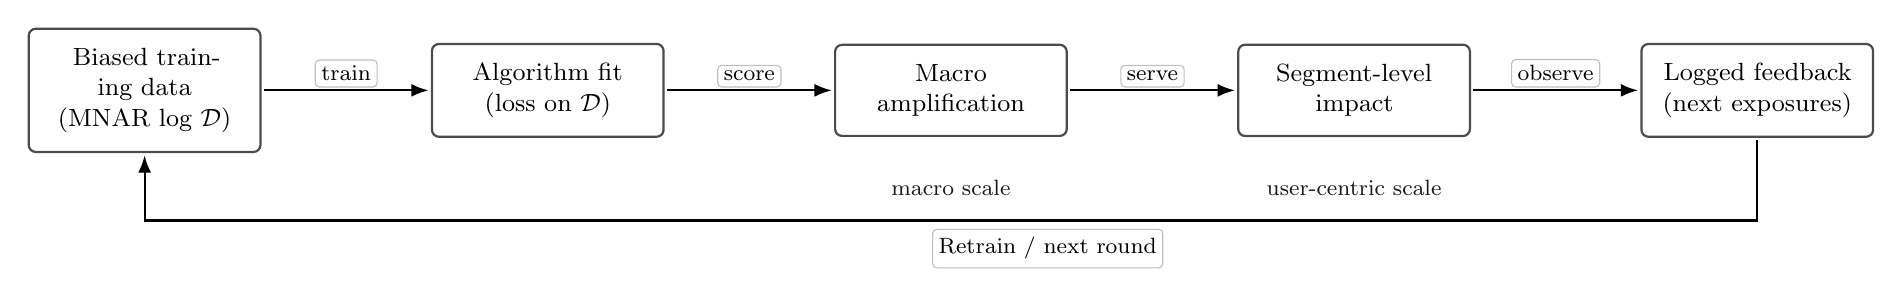
\begin{tikzpicture}[
    font=\small,
    box/.style={rectangle, draw=black!70, rounded corners=2.5pt, thick, align=center, inner sep=7pt, minimum height=1.05cm, text width=2.45cm},
    edgelab/.style={font=\footnotesize, text=black, text opacity=1, fill=white, inner sep=2.2pt, rounded corners=1.5pt, draw=black!25, thin},
    scl/.style={font=\footnotesize, text=black!90},
    arr/.style={-{Latex[length=2.2mm]}, thick, shorten >=0.8pt, shorten <=0.8pt}
  ]
    \node[box] (mnar) {Biased training data\\(MNAR log $\mathcal{D}$)};
    \node[box, right=2.15cm of mnar] (fit) {Algorithm fit\\(loss on $\mathcal{D}$)};
    \node[box, right=2.15cm of fit] (macro) {Macro\\amplification};
    \node[box, right=2.15cm of macro] (user) {Segment-level\\impact};
    \node[box, right=2.15cm of user] (log) {Logged feedback\\(next exposures)};
    \draw[arr] (mnar) -- node[above, edgelab, yshift=1pt] {train} (fit);
    \draw[arr] (fit) -- node[above, edgelab, yshift=1pt] {score} (macro);
    \draw[arr] (macro) -- node[above, edgelab, yshift=1pt] {serve} (user);
    \draw[arr] (user) -- node[above, edgelab, yshift=1pt] {observe} (log);
    \draw[arr] (log.south) -- ++(0,-1.05) -| node[pos=0.22, below, edgelab, yshift=-3pt] {\strut Retrain / next round} (mnar.south);
    \node[scl, anchor=north] at ($(macro.south)+(0,-0.42)$) {macro scale};
    \node[scl, anchor=north] at ($(user.south)+(0,-0.42)$) {user-centric scale};
  \end{tikzpicture}%
  }
  \caption{The \emph{Bias Propagation Chain}: MNAR training data and exposure-coupled objectives produce macro-level concentration, uneven segment-level service, and feedback-generated logs that re-enter training. Macro diagnostics, user-centric tests, and longitudinal simulation (Experiments A--C) interrogate successive links of the same loop.}
  \label{fig:bias_propagation_chain}
\end{figure}

%                      -
\subsection{Constructs and formal definitions}
\label{sec:lit_theory_constructs}

Before proceeding to the hypotheses and experimental design, it is important to establish precise, consistent definitions for the key constructs used throughout this thesis. The popularity bias literature is unfortunately inconsistent in its terminology: different papers use the terms ``popularity bias,'' ``exposure bias,'' and ``diversity'' in overlapping and sometimes contradictory ways. This creates a risk of conceptual confusion when comparing results across studies. The definitions below fix the meaning of each construct as it is used in this thesis, distinguishing carefully between bias that originates in the \emph{training data}, bias that arises from \emph{how the model surfaces items at decision time}, disparities in \emph{service quality across user segments}, and changes in \emph{aggregate recommendation diversity over time}. These are related but distinct phenomena, and conflating them obscures the causal structure that the Bias Propagation Chain is designed to make explicit.

\textbf{Popularity bias (training distribution).}
Let $f_i$ denote the empirical frequency or, in the case of implicit feedback, the raw interaction count of item $i$ in the logged interaction matrix $\mathcal{D}$. Popularity bias is the structural \emph{over-representation} of items with high $f_i$ relative to the reference distribution that would arise under a hypothetical unbiased data-collection process for example, if every user had been randomly exposed to every item with equal probability. This is a property of the \emph{data generating process} that produces $\mathcal{D}$. It exists before any particular recommendation model has been trained, and it is the primary source of skew that all downstream algorithmic decisions inherit. Crucially, items with high $f_i$ are not necessarily \emph{better} than items with low $f_i$; they are simply items that the platform's historical exposure policy happened to surface to more users, giving them more opportunities to accumulate interactions.

\textbf{Exposure bias (surfacing and missingness).}
For a given user $u$, let $P_u$ denote the \textbf{latent full-information preference distribution} the distribution over items that describes what this user would prefer \emph{if they had been exposed to every item and had the opportunity to form a genuine opinion about it}. In practice, this distribution is never directly observable. What we observe instead is shaped by $E_u$, the \textbf{platform exposure distribution}: the distribution over items that the platform actually surfaces to user $u$ during the data collection period. The interactions we record for user $u$ are draws from the intersection of $P_u$ and $E_u$ items the user both prefers and was exposed to. Exposure bias names the systematic wedge between $P_u$ (what the user truly prefers) and $E_u$ (what the system surfaces), including the consequence that large regions of the item catalog are simply never represented in $\mathcal{D}$ for most users \citep{marlin2009mnar, schnabel2016ips}. This is the recommender-system specialisation of MNAR: the probability that a user-item pair is observed in $\mathcal{D}$ depends on the user's latent preference for the item \emph{and} on the platform's historical decision to expose that item to that user. Exposure bias is therefore not reducible to ``the model likes popular items.'' It is the causal structure upstream of any model, embedded in the data collection process itself, that makes popular items far likelier to appear in $\mathcal{D}$ regardless of true user preferences.

\textbf{Niche tax (segment-level service gap).}
Users can be partitioned into cohorts based on how closely their historical interaction profiles overlap with the globally popular items on the platform. This measure is called \textbf{mainstreaminess} \citep{abdollahpouri2021usercentered}: a user with high mainstreaminess prefers items that are widely popular across the platform; a user with low mainstreaminess (a ``niche user'') prefers items that most other users rarely interact with. The \textbf{niche tax} is the systematic difference in recommendation quality measured by metrics such as prediction error (RMSE) or ranking quality (NDCG@$K$) between niche users and mainstream users, when both groups are evaluated under the \emph{same} model and experimental protocol. A positive niche tax means niche users receive systematically worse recommendations: their predictions are less accurate, and the items ranked highest for them are less relevant to their actual preferences. The niche tax is an \emph{outcome disparity} metric. It does not measure a property of the data alone or a property of the model alone; it measures the \emph{interaction} between the structural biases in the data and the inductive assumptions of the model, as experienced by different groups of users.

\textbf{Diversity decay (longitudinal).}
Let $R^{(t)}$ denote the \textbf{multiset} of recommended items at feedback round $t$ that is, the collection of all items appearing in all recommendation lists generated at round $t$, aggregated across all users (where the same item can appear multiple times if it is recommended to multiple users). Diversity decay is the reduction, over increasing rounds $t$, in \emph{dispersion indices} computed on $R^{(t)}$. Dispersion indices are metrics that measure how spread out or concentrated a distribution is. In this context, relevant dispersion indices include catalogue coverage (the fraction of all available items that appear in at least one recommendation list) and the Gini coefficient of item recommendation frequencies. A system exhibiting diversity decay shows falling catalogue coverage and rising Gini over successive feedback rounds, holding the simulation protocol constant \citep{mansoury2020feedback, chaney2018algorithmic}. Diversity decay is a \emph{dynamic} construct: it can only be measured over time and requires a longitudinal evaluation protocol, which is why Experiment~C of this thesis employs a multi-round feedback simulation rather than a single-snapshot evaluation.

\textbf{Catalog starvation (extreme macro manifestation).}
Catalog starvation is the \emph{limiting case} of diversity decay: the regime in which the recommended support the set of items that ever appear in any recommendation list collapses to a vanishing fraction of the full catalog. In practical terms, a system in a state of catalog starvation is recommending the same tiny set of extremely popular items to virtually every user, regardless of their individual preferences. This represents a complete failure of the system's core function: personalised discovery. What makes catalog starvation particularly insidious is that standard accuracy metrics can remain deceptively stable even as it occurs. If the few items being recommended happen to be genuinely popular with most users, average RMSE and Precision@K can look acceptable on aggregate the aggregate metric is dominated by the majority of users whose mainstream tastes are being served while niche users receive uniformly poor recommendations and the vast majority of the catalog is effectively invisible \citep{steck2011itempopularity}. Catalog starvation is the macro-level endpoint of the Bias Propagation Chain under conditions of extreme sparsity and strong collaborative amplification, and it is documented empirically for the Takealot corpus in Experiment~A (Chapter~\ref{ch:exp_a}).

Figure~\ref{fig:theory_construct_map} situates these five constructs in relation to one another, showing how training-side skew and decision-time missingness feed segment-level disparities, which feed longitudinal dynamics, with catalog starvation as the extreme limiting outcome.

\begin{figure}[htbp]
  \centering
  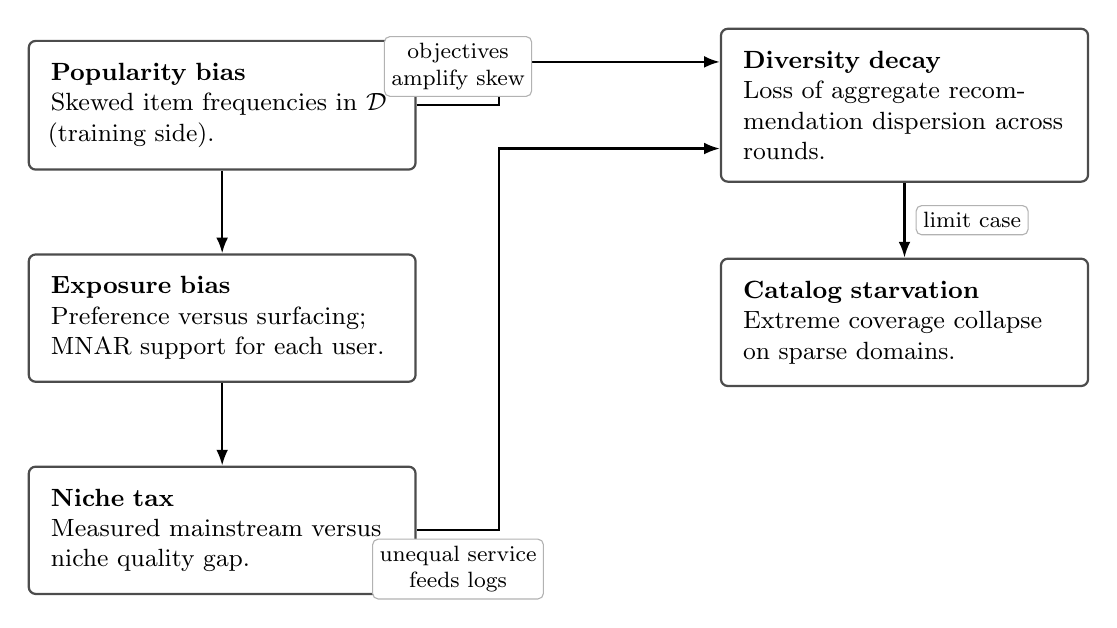
\begin{tikzpicture}[
    font=\small,
    box/.style={draw=black!70, rounded corners=2.5pt, thick, align=left, inner sep=8pt, text width=4.35cm},
    arr/.style={-{Latex[length=2mm]}, thick},
    arrlab/.style={font=\footnotesize, text=black, text opacity=1, align=center, fill=white, inner sep=2.5pt, rounded corners=2pt, draw=black!30, thin}
  ]
    \node[box] (pb) {\textbf{Popularity bias}\\Skewed item frequencies in $\mathcal{D}$ (training side).};
    \node[box, below=1.05cm of pb] (eb) {\textbf{Exposure bias}\\Preference versus surfacing; MNAR support for each user.};
    \node[box, below=1.05cm of eb] (nt) {\textbf{Niche tax}\\Measured mainstream versus niche quality gap.};
    \node[box, right=3.85cm of pb, text width=4.1cm] (dd) {\textbf{Diversity decay}\\Loss of aggregate recommendation dispersion across rounds.};
    \node[box, below=0.95cm of dd, text width=4.1cm] (cs) {\textbf{Catalog starvation}\\Extreme coverage collapse on sparse domains.};
    \coordinate (ddinup) at ($(dd.west)+(0,0.55)$);
    \coordinate (ddinlo) at ($(dd.west)+(0,-0.55)$);
    \draw[arr] (pb) -- (eb);
    \draw[arr] (eb) -- (nt);
    \draw[arr] (pb.east) -- ++(1.05,0) coordinate (pbstub) |- (ddinup);
    \path (pb.east) -- (pbstub) node[midway, above=3pt, arrlab] {objectives\\amplify skew};
    \draw[arr] (nt.east) -- ++(1.05,0) coordinate (ntstub) |- (ddinlo);
    \path (nt.east) -- (ntstub) node[midway, below=3pt, arrlab] {unequal service\\feeds logs};
    \draw[arr] (dd) -- node[right, arrlab, xshift=4pt] {limit case} (cs);
  \end{tikzpicture}
  \caption{Relations among constructs used in this thesis: training-side popularity skew and exposure-coupled missingness shape segment-level disparities; feedback and retraining link user-level outcomes to longitudinal diversity loss, with catalog starvation as the extreme macro outcome.}
  \label{fig:theory_construct_map}
\end{figure}

%                      -
\subsection{Hypotheses}
\label{sec:lit_theory_hyp}

Research Questions 1--3 (Chapter~\ref{ch:introduction}) are reframed here as directional hypotheses derived from the Bias Propagation Chain. The word ``directional'' is important: these are not claims that an effect exists or does not exist, but claims about the \emph{direction} of an effect which model family will exhibit more concentration, which user group will receive worse recommendations, which trajectory will show more diversity decay. Each hypothesis maps directly to one experiment.

\textbf{H1 (Experiment~A, RQ1).}
The theoretical mechanism described in Section~\ref{sec:lit_theory_chain} predicts that collaborative latent-factor and implicit models, by minimising squared or implicit-feedback loss on MNAR training data with a popularity-skewed support set, will concentrate their recommendations on head items more strongly than content-based models. Content-based models, whose predictions depend on item feature similarity rather than on interaction frequency, are structurally decoupled from the co-occurrence counts that drive popularity amplification in collaborative systems. Their features are not monotone functions of interaction counts a niche item with a rich text description receives the same quality of feature representation as a popular item with an equally rich description.

\emph{Directional prediction:} Collaborative latent-factor (SVD) and implicit (ALS) baselines will exhibit higher Gini coefficients, higher ARP, and lower catalogue coverage than TF--IDF, logistic regression, and random forest baselines under matched experimental protocols. This gap is expected to widen under extreme sparsity (Takealot), where the thin support for niche items makes collaborative amplification most severe.

\textbf{H2 (Experiment~B, RQ2).}
The niche tax arises because niche users draw on thinner collaborative neighbourhoods and provide fewer reliable training signals for the latent factors that describe their preferred items. Mainstream users, by contrast, align closely with the dense region of the training support, where the model has abundant evidence and produces confident, accurate predictions.

\emph{Directional prediction:} Niche user cohorts will exhibit statistically higher RMSE and lower NDCG@10 than mainstream cohorts under user-based $k$-NN, biased matrix factorisation (SVD), and implicit ALS. The gap is expected to be smaller, or even reversed, for content-based pipelines that partially decouple predictions from global co-occurrence, because content models can score a niche item for a niche user based on feature similarity even when interaction data is sparse.

\textbf{H3 (Experiment~C, RQ3).}
When a collaborative filtering model is retrained on interaction logs generated by its own prior recommendations, the feedback loop described in Section~\ref{sec:lit_theory_chain} predicts a progressive increase in popularity concentration. The model reinforces its own exposure policy: it recommends popular items, users interact with those items, those interactions enter the training log, and the next model places even higher confidence on popular items. Content-based models, which rely on item-feature similarity rather than on estimating popularity from the interaction graph, are predicted to be more resilient to this feedback-driven concentration because their scoring mechanism does not depend on the volume of interactions an item has accumulated.

\emph{Directional prediction:} SVD trajectories will show non-decreasing ARP and non-increasing catalogue coverage across five simulated feedback rounds. TF--IDF trajectories will show flatter or recovering diversity trajectories under the same shared click simulator. The contrast between the two model families under identical simulation conditions will constitute a controlled test of whether collaborative versus content-based inductive biases lead to qualitatively different long-run behaviours.

%                      -
\subsection{The Sparsity Amplification Conjecture}
\label{sec:lit_theory_sparsity}

Beyond the three main hypotheses, this thesis advances a cross-cutting theoretical conjecture that applies to all three experiments simultaneously: \textbf{sparsity amplifies every link in the Bias Propagation Chain}.

To understand why, consider what happens to each stage of the chain when the interaction density of the training data drops dramatically as it does when moving from the MovieLens benchmark (where the average user has rated dozens of films) to the Takealot corpus (where the average user has interacted with only a handful of products from a catalog of tens of thousands).

At the \textbf{data level}, sparsity makes the MNAR problem more acute. When interaction counts per item are small, each additional appearance of a popular head item constitutes a larger fraction of the total available evidence. The popularity skew in $\mathcal{D}$ becomes statistically sharper relative to the noise floor the signal-to-noise ratio for niche items deteriorates, making it even harder to distinguish genuine niche preference from random sampling variation.

At the \textbf{model level}, sparsity degrades the quality of latent factor estimates for niche items. A matrix factorisation model trained on a dense dataset can triangulate the position of a niche item in the latent space from dozens of user interactions. On a sparse dataset, that item may have only one or two interactions, making its latent vector poorly defined and highly sensitive to the specific users who happened to interact with it. Optimisers trained under sparsity tend to collapse toward frequency-shaped solutions configurations where the latent factors are dominated by popularity rather than by genuine taste dimensions because popularity is the only signal strong enough to be reliably estimated from thin data \citep{steck2010training}.

At the \textbf{user level}, sparsity tightens the niche tax. Niche users meet fewer reliable collaborative neighbours in sparse environments, because the items they prefer also have sparse interaction records. The model's predictions for niche users become not just biased but actively unreliable. Post-processing mitigations that do not inject new propensity information into the training process reranking the model's existing output cannot repair this underlying unreliability, because they have no way to conjure signal that was never collected \citep{abdollahpouri2019managing}.

The practical implication of this conjecture is significant: results obtained on dense academic benchmarks like MovieLens may substantially underestimate the severity of popularity bias in real-world deployments. Dense benchmarks produce bias that is \emph{mechanically dampened} by abundant interaction counts, which smooth out the extreme concentration effects that emerge when the same algorithm is deployed on a sparse retail catalog. This is why the Takealot corpus is included in this study not as a curiosity, but as a deliberate \textbf{stress test} that exposes the full severity of the Bias Propagation Chain under conditions that are representative of real e-commerce deployment. The conjecture is evaluated across Chapters~\ref{ch:exp_a}--\ref{ch:exp_c} by comparing the direction and magnitude of bias metrics on public dense benchmarks against those observed on the Takealot corpus.
%   - 2.7 ending of theoretical framework
\section{The research gap}
\label{sec:lit_gap}

The preceding sections of this chapter have established a substantial body of knowledge about popularity bias in recommender systems. Researchers understand, in broad terms, why bias enters the training data (MNAR), how different algorithmic families amplify it, how it falls unevenly across user segments, and how it compounds over time through feedback loops. Mitigation strategies have been proposed at every stage of the pipeline. Comprehensive surveys have catalogued dozens of definitions, metrics, and correction techniques \citep{klimashevskaia2024survey}.

And yet, despite this breadth of existing work, a specific and practically important combination of research dimensions has not been addressed as a single, unified empirical programme. This section makes that gap precise. It is not enough to gesture vaguely at ``more work needed'' a credible claim of novelty requires identifying exactly which combinations of dimensions are missing, why those combinations matter, and how the present study fills them. The five claims below do exactly that. Each claim identifies a specific limitation in the existing literature, explains why that limitation matters for understanding bias in real-world systems, and states what this thesis does to address it.

Table~\ref{tab:lit_gap} provides an at-a-glance summary of how representative foundational papers cover four key evaluation dimensions: macro-level exposure bias, user-centric fairness, longitudinal feedback dynamics, and sparse e-commerce stress testing. The cells marked ``Y'' indicate that a paper addresses a dimension fully and centrally; ``(Y)'' indicates partial or incidental coverage; an empty cell indicates the dimension is not a focus of the work. The final row shows the coverage claimed by this thesis.

\begin{table}[htbp]
  \centering
  \caption{Illustrative coverage of key dimensions in selected prior work 
  (Y\,=\,addressed; (\,Y\,)\,=\,partial; empty\,=\,not central). 
  The final row sketches this thesis.}
  \label{tab:lit_gap}
  \begin{tabular}{@{}lcccc@{}}
    \toprule
    \textbf{Reference} & \textbf{Macro} & \textbf{User} & \textbf{Dynamic} & \textbf{Sparse e-com.} \\
    \midrule
    \citeauthor{abdollahpouri2019unfairness} \citeyearpar{abdollahpouri2019unfairness} 
      & Y & (\,Y\,) & & \\
    \citeauthor{abdollahpouri2021usercentered} \citeyearpar{abdollahpouri2021usercentered} 
      & (\,Y\,) & Y & & \\
    \citeauthor{mansoury2020feedback} \citeyearpar{mansoury2020feedback} 
      & (\,Y\,) & & Y & \\
    \citeauthor{chaney2018algorithmic} \citeyearpar{chaney2018algorithmic} 
      & (\,Y\,) & & Y & \\
    \citeauthor{klimashevskaia2024survey} \citeyearpar{klimashevskaia2024survey} 
      & Y & Y & (\,Y\,) & (\,Y\,) \\
    \midrule
    \textbf{This thesis} & Y & Y & Y & Y \\
    \bottomrule
  \end{tabular}
\end{table}

Reading across the rows of Table~\ref{tab:lit_gap} reveals the core pattern: no single prior work achieves full coverage across all four dimensions simultaneously. Each paper addresses one or two dimensions well, and either ignores the others or treats them incidentally. This is not a criticism of those papers each was designed to answer a specific research question, and each does so rigorously. The limitation is structural: the field has accumulated deep but narrow studies, and the intersections between dimensions have been left largely unexplored. The five claims below explain each missing intersection in detail.

\vspace{0.75em}
\noindent\textbf{Claim 1: Isolated algorithmic paradigms.}

Most foundational papers on popularity bias in recommender systems focus primarily or exclusively on \emph{collaborative filtering} algorithms \citep{abdollahpouri2019unfairness, mansoury2020feedback}. This is understandable collaborative filtering is the dominant paradigm in production recommender systems, and it is the family of algorithms most obviously vulnerable to popularity amplification through co-occurrence statistics and latent factor estimation. However, this focus on collaborative methods means that the field lacks a clear, controlled understanding of how bias compares \emph{across} fundamentally different algorithmic families.

Specifically, there is a shortage of studies that place memory-based collaborative methods ($k$-NN), model-based collaborative methods (SVD, ALS), and content-based methods (TF--IDF profiling, logistic regression, random forests) side by side, train them all on the same data under identical preprocessing and evaluation conditions, and then compare their bias profiles on the same set of metrics. Without this kind of controlled comparison, it is impossible to make clean, causal claims about whether a particular bias pattern is a consequence of the \emph{collaborative paradigm as a whole}, or of the specific \emph{architecture} within that paradigm (neighbourhood-based versus latent-factor), or simply of the dataset being used. The few comparative studies that do exist typically vary their experimental conditions in ways that make direct comparisons difficult different datasets, different preprocessing steps, different metric definitions obscuring the precise contribution of algorithmic architecture to bias amplification.

This matters practically because a system designer choosing between algorithmic families needs to know how that choice will affect the bias profile of the deployed system, not just its accuracy. Claim~1 motivates the comparative design of Experiment~A, which trains all six baseline families on all five datasets under a single unified protocol and reports bias metrics side by side.

\vspace{0.75em}
\noindent\textbf{Claim 2: Dense-benchmark dominance.}

The offline evaluation literature in recommender systems is heavily concentrated on a small number of well-known academic benchmark datasets. MovieLens (in its various sizes), Last.fm, and related corpora dominate the published results in popularity bias research \citep{klimashevskaia2024survey}. These datasets share an important characteristic: they are relatively \emph{dense} by the standards of real-world deployments. MovieLens users have typically rated tens or hundreds of films; Last.fm users have accumulated thousands of play counts. The interaction matrices, while technically sparse in the mathematical sense (most user-item pairs are unobserved), are dense enough that most items have at least a few interactions and most users have a meaningful interaction history.

This density profile is qualitatively different from what is encountered in real e-commerce environments. A large online retail platform may stock hundreds of thousands or millions of distinct products (SKUs), while the typical customer purchases only a handful of items per year. The resulting interaction matrix is not just sparse it is \emph{ultra-sparse}, with interaction densities orders of magnitude lower than those of MovieLens. In this regime, the mechanisms through which popularity bias operates are qualitatively different: the thin tail of niche items is effectively invisible to collaborative algorithms, latent factor estimation becomes unreliable for the vast majority of the catalog, and neighbourhood-based methods can collapse to recommending only a handful of globally popular items to every user regardless of their individual preferences.

Published results on dense benchmarks therefore cannot safely be extrapolated to real-world deployments. A model that shows acceptable Gini coefficients and reasonable coverage on MovieLens may exhibit catastrophic catalog starvation when deployed on a retail platform. The existing literature provides very little empirical guidance on how severe this gap is, because ultra-sparse retail datasets are proprietary and rarely shared. Claim~2 motivates the inclusion of the Takealot corpus in this study a large, proprietary, ultra-sparse e-commerce dataset that serves as a domain stress test for all six algorithmic families, revealing failure modes that are invisible on academic benchmarks.

\vspace{0.75em}
\noindent\textbf{Claim 3: Split metrics across separate studies.}

A persistent structural problem in the popularity bias literature is that macro-level exposure studies and user-centric fairness studies tend to appear in \emph{separate} papers, using \emph{different} algorithm lists, \emph{different} datasets, and \emph{different} metric definitions. Papers focused on macro-level bias measuring Gini coefficients, catalogue coverage, and average recommendation popularity across the full item catalog rarely also report how these concentration patterns translate into differential service quality for different user segments. Papers focused on user-centric fairness measuring RMSE gaps and NDCG disparities between mainstream and niche user cohorts rarely also report the full macro-level exposure distribution that underlies those disparities.

This separation makes it very difficult to understand the \emph{relationship} between macro concentration and user-level impact. Is a system with a Gini coefficient of 0.9 necessarily one that imposes a severe niche tax? Does a system with a small RMSE gap between niche and mainstream users also tend to have reasonable catalogue coverage? These questions cannot be answered by looking at macro studies and user studies separately they require a unified table that reports both types of metrics for the same algorithm evaluated on the same data under the same protocol.

Such a unified table is still uncommon in the literature. Claim~3 motivates the joint reporting design of this thesis: every algorithm evaluated in Experiment~A (macro metrics: Gini, coverage, ARP, Spearman correlation, long-tail share) is also evaluated in Experiment~B (user-centric metrics: RMSE and NDCG@10 by mainstreaminess segment), so that the relationship between catalog-level concentration and segment-level disparity can be studied directly.

\vspace{0.75em}
\noindent\textbf{Claim 4: Feedback simulations that omit content-based models.}

The existing literature on feedback loops and longitudinal bias dynamics has focused almost exclusively on collaborative filtering algorithms \citep{chaney2018algorithmic, mansoury2020feedback, jiang2019degenerate}. This is the natural starting point collaborative methods are the ones most obviously susceptible to feedback-driven popularity amplification, because their predictions depend on interaction counts that are themselves shaped by the system's prior recommendations. But this exclusive focus on collaborative methods leaves an important methodological question unanswered: how do content-based models behave under the same feedback conditions?

Content-based models are structurally different in a way that is theoretically relevant to feedback dynamics. Their predictions depend on item feature similarity the text, metadata, or attribute overlap between items rather than on the volume of interactions those items have accumulated. This structural decoupling from interaction counts suggests that content-based models may be more resilient to feedback-driven popularity amplification: even if the system repeatedly recommends popular items and those interactions dominate the training log, a content-based model's scoring of niche items is not directly degraded, because niche items' feature representations do not depend on how many times they have been interacted with.

Whether this theoretical resilience holds in practice under a realistic stochastic click model that mixes relevance and popularity signals is an open empirical question. Directly contrasting collaborative (SVD) and content-based (TF--IDF) feedback trajectories under a \emph{shared} click simulator, on the same user population and item catalog, is what makes it possible to attribute observed differences in longitudinal behaviour to algorithmic architecture rather than to dataset or simulation artefacts. Claim~4 motivates the design of Experiment~C, which runs five-round feedback simulations for both SVD and TF--IDF under identical conditions and compares how their aggregate diversity and average recommendation popularity evolve over iterations.

\vspace{0.75em}
\noindent\textbf{Claim 5: Stress-testing sparsity as an explanatory variable.}

Even papers that acknowledge the importance of dataset sparsity typically treat it as a \emph{confound to be controlled for} rather than as an \emph{explanatory variable to be studied}. The standard approach is to apply $k$-core filtering removing users and items with fewer than $k$ interactions to bring all datasets to a comparable minimum density before evaluation. This is methodologically sound for the purpose of ensuring stable model estimates, but it systematically discards exactly the regime that is most relevant to real-world deployments: the ultra-sparse tail.

When the results of this thesis show that ALS on the Takealot corpus achieves a Gini coefficient of $0.9998$ and recommends only 14 distinct items across the entire test cohort, the correct interpretation is not ``ALS performs poorly on this dataset.'' The correct interpretation, grounded in the MNAR framework and the Sparsity Amplification Conjecture of Section~\ref{sec:lit_theory_sparsity}, is that \emph{extreme sparsity exposes a fundamental failure mode of implicit collaborative filtering that dense benchmarks mechanically suppress}. The failure is not accidental or implementation-specific it is a predictable consequence of applying confidence-weighted implicit feedback objectives to a dataset where niche items have near-zero training support. Dense benchmarks dampen this effect by providing enough interactions for most items that the model can form at least crude estimates of their properties. Ultra-sparse retail data strips away that cushion and reveals the algorithm's behaviour at its limit.

This interpretive frame treating sparsity as an amplifier of the Bias Propagation Chain rather than as a nuisance variable is what Claim~5 contributes. Without a proprietary ultra-sparse corpus to stress-test against, the conclusions of this study would be limited to the regime that academic benchmarks cover, and the most practically important failure modes would remain invisible.

\vspace{0.75em}
\noindent\textbf{Mapping claims to experiments.}

The five claims above are not independent observations they are facets of a single structural gap in the literature, and together they define the contribution of this thesis as a \emph{unified empirical programme} rather than a collection of loosely related studies.

Experiment~A (Chapter~\ref{ch:exp_a}) directly addresses Claims~1 and 2 by evaluating all six algorithmic families on all five datasets under a single unified protocol and reporting macro-level concentration metrics side by side. The controlled comparison across paradigms closes Claim~1; the inclusion of the Takealot corpus closes Claim~2.

Experiment~B (Chapter~\ref{ch:exp_b}) addresses Claim~3 by reporting user-centric fairness metrics (RMSE and NDCG@10 by mainstreaminess segment) for the same algorithms evaluated in Experiment~A, enabling direct comparison between macro-level exposure patterns and segment-level service quality within a single study.

Experiment~C (Chapter~\ref{ch:exp_c}) addresses Claim~4 by running longitudinal feedback simulations for both collaborative (SVD) and content-based (TF--IDF) models under identical click-generation conditions, producing the first direct controlled comparison of how these two algorithmic families respond to feedback-driven popularity reinforcement.

The Takealot corpus, present in all three experiments, addresses Claim~5 throughout by providing the ultra-sparse domain stress test that reveals failure modes suppressed by academic benchmark density.

Together, these four experimental components instantiate the intersection that no prior single study has covered: \emph{algorithmic bias across paradigms, user-group fairness, and longitudinal dynamics}, all evaluated coherently under a shared protocol, with ultra-sparse e-commerce data as a counterpoint to the dense textbook benchmarks that dominate the existing literature. This is the specific, bounded, and practically motivated contribution that this thesis makes to the recommender systems research community.

%  - ending of the overall gap
\chapter{Methodology and Experimental Framework}
\label{ch:methodology}

This chapter presents the complete methodological blueprint of the thesis. It describes the research design and the rationale for its three-phase structure, characterises the datasets used and the preprocessing decisions applied to them, defines the full suite of evaluation metrics, specifies the algorithmic baselines and their hyperparameter choices, details the statistical testing framework, and documents the known limitations and threats to validity of the experimental design. Together, these components constitute a fully reproducible empirical framework for measuring popularity bias across heterogeneous dataset domains.

%                      -
\section{Research Design Overview}
\label{sec:method_design}

The central empirical goal of this thesis is to produce a rigorous, comparative quantification of popularity bias across six algorithmically distinct recommendation architectures and five datasets that span a wide spectrum of interaction density from the dense, well-curated MovieLens benchmarks to an extremely sparse proprietary e-commerce catalog. To achieve this goal in a way that is both internally valid and practically interpretable, the study adopts a three-phase experimental pipeline, illustrated in Figure~\ref{fig:pipeline}.

The three experiments are not independent modules; they are a deliberately ordered sequence in which each phase addresses a dimension of bias that the previous phase cannot capture alone.

\begin{enumerate}
    \item \textbf{Experiment A   Macro-Level Exposure Bias:} The first phase characterises the distributional properties of each algorithm's recommendation output at the catalog level. It asks: how unequally are items exposed across the full recommendation surface? How much of the available catalog does each algorithm actually utilise? What is the average popularity of recommended items? These questions are answered using Gini coefficients, catalog coverage, average recommendation popularity (ARP), and exposure entropy, computed across all users. Experiment A establishes the baseline bias fingerprint of each algorithm before any user-level or temporal analysis is introduced.

    \item \textbf{Experiment B   User-Centric Fairness:} The second phase disaggregates the macro-level picture by partitioning users into segments according to their mainstreaminess the degree to which their historical preferences overlap with globally popular items. It asks: does popularity bias fall equally on all users, or do users with niche preferences bear a disproportionate accuracy penalty? Group Average Popularity (GAP), $\Delta$GAP, and segment-level NDCG and RMSE are computed separately for mainstream, diverse, and niche user groups, and the distributions are compared using non-parametric statistical tests. Experiment B reveals the consumer-side fairness consequences of the macro-level biases documented in Experiment A.

    \item \textbf{Experiment C   Longitudinal Feedback Dynamics:} The third phase introduces the temporal dimension. Using a synthetic click simulator, it subjects each algorithm to multiple rounds of the recommend-observe-retrain cycle and tracks how the distributional metrics from Experiment A and the segment disparities from Experiment B evolve over time. It asks: does popularity bias compound through feedback, and do different algorithmic architectures amplify or resist this compounding at different rates? Without this phase, the static bias measurements from Experiments A and B could not be interpreted in the context of real-world deployment, where models are continuously retrained on interaction data that is itself shaped by prior recommendations.
\end{enumerate}

This three-phase structure ensures that the thesis measures bias at three distinct levels of analysis catalog-wide, user-segment-level, and longitudinal using a consistent set of metrics and the same six algorithm families throughout, enabling direct cross-experiment comparison.

\begin{figure}[htbp]
  \centering
  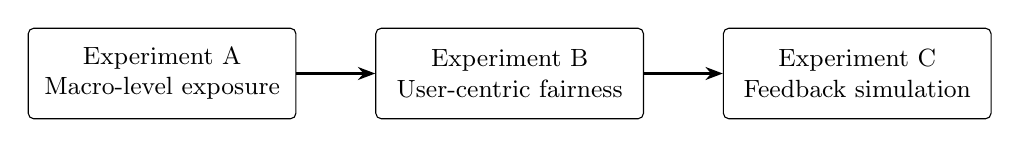
\begin{tikzpicture}[
      node distance=0.6cm and 1.0cm,
      box/.style={rectangle, draw, rounded corners=2pt, minimum width=3.4cm, minimum height=1.15cm, align=center, font=\small},
      arr/.style={-{Stealth[length=2.2mm]}, thick},
    ]
    \node[box] (a) {Experiment A\\Macro-level exposure};
    \node[box, right=of a] (b) {Experiment B\\User-centric fairness};
    \node[box, right=of b] (c) {Experiment C\\Feedback simulation};
    \draw[arr] (a) -- (b);
    \draw[arr] (b) -- (c);
  \end{tikzpicture}
  \caption{The three-phase experimental pipeline. Each phase addresses a dimension of popularity bias that the preceding phase cannot capture in isolation.}
  \label{fig:pipeline}
\end{figure}

%                      -
\section{Datasets and Domains}
\label{sec:method_datasets}

A central design decision of this thesis is to evaluate all algorithms across multiple datasets that vary substantially in their interaction density, domain, and feedback type. The academic recommender systems literature is dominated by a small number of dense, well-curated benchmark datasets most prominently MovieLens which have sparsity profiles that are considerably more favourable than those encountered in real-world e-commerce. Relying on these benchmarks alone would produce conclusions that may not generalise to the sparse, long-tailed interaction regimes characteristic of deployed retail recommendation systems. To address this, the study uses four public benchmark datasets and one proprietary e-commerce dataset, described below and summarised in Table~\ref{tab:datasets}.

\subsection*{Public Benchmark Datasets}

\textbf{MovieLens 100K and MovieLens 1M} \citep{harper2015movielens} are the most widely used benchmarks in recommendation research. Both contain explicit star ratings (1--5) from users of the GroupLens movie recommendation service. The 100K variant contains 100,000 ratings from 943 users across 1,682 films; the 1M variant scales this to approximately 1,000,209 ratings from 6,040 users across 3,900 films. Both datasets are relatively dense by recommender systems standards their interaction matrices are far less sparse than typical e-commerce data and they carry clean, structured item metadata in the form of genre labels. These properties make them useful as controlled reference points: if an algorithm exhibits a particular bias behaviour on MovieLens but not on sparser datasets, the difference is attributable to interaction density rather than domain-specific factors.

\textbf{Last.fm 2K} \citep{cantador2011second} is a music listening dataset containing implicit feedback in the form of play counts the number of times each user has listened to each artist. Unlike the MovieLens datasets, which contain explicit ratings, Last.fm captures behavioural engagement without any explicit preference signal. For compatibility with the evaluation framework, raw play counts are discretised into five ordinal rating bins, preserving the ordinal structure of engagement intensity while enabling the same rating-prediction pipeline to be applied. Item metadata is constructed by concatenating artist names with user-assigned tags, producing a text representation suitable for content-based models. Last.fm represents an intermediate sparsity regime between the dense MovieLens benchmarks and the e-commerce catalog.

\textbf{Book-Crossing} \citep{ziegler2005improving} is a book rating dataset collected from the Book-Crossing community, containing both explicit ratings (scale 1--10) and implicit zero ratings that represent awareness without explicit preference. The dataset is substantially sparser than MovieLens, and its long-tailed popularity distribution in which a small number of bestselling titles account for the large majority of interactions makes it a useful proxy for the catalog concentration dynamics observed in e-commerce. For this thesis, implicit zero ratings are removed, retaining only interactions that carry an explicit preference signal, to ensure that accuracy metrics reflect genuine preference estimates rather than the confounded signal of implicit non-ratings.

\subsection*{Proprietary E-Commerce Dataset (Takealot)}

The primary empirical contribution of this thesis is the evaluation of all six algorithm families on a large, proprietary interaction dataset from Takealot, one of southern Africa's largest e-commerce platforms. This dataset was provided under a data access agreement for academic research purposes. All records are fully anonymised: user identifiers and product identifiers are pseudonymised, and no personally identifiable information is retained in the analysis dataset.

The Takealot dataset represents a qualitatively different challenge from all four public benchmarks. Its defining characteristics are:

\begin{itemize}
    \item \textbf{Extreme sparsity:} The interaction matrix is orders of magnitude sparser than any of the public benchmarks. The vast majority of user-product pairs have zero interactions, and most users have purchased or reviewed only a handful of products from a catalog spanning hundreds of thousands of SKUs (stock-keeping units).
    \item \textbf{Severely long-tailed popularity:} A small fraction of products bestselling consumer electronics, popular household items, and promotional SKUs account for a disproportionate share of all recorded interactions. The tail of the product catalog, containing the majority of available SKUs, has extremely thin interaction support.
    \item \textbf{Implicit feedback structure:} The interaction signal is derived from customer reviews, which represent a form of post-purchase engagement rather than explicit preference elicitation. This makes the data MNAR (Missing Not At Random) by construction: the probability of leaving a review is correlated with satisfaction, which is itself correlated with item quality and visibility.
    \item \textbf{Rich product metadata:} Item representations are constructed by concatenating product names, brand names, and store category paths, producing a structured text corpus suitable for TF-IDF and content-based models.
\end{itemize}

The Takealot dataset serves as the primary stress test for all six algorithm families. Its sparsity profile exposes failure modes such as the ALS instability and neighborhood collapse documented in the results that would not be visible on the denser public benchmarks, and it provides the ecologically valid context that motivates the thesis's focus on extreme-sparsity recommender behaviour.

\begin{table}[htbp]
\centering
\caption{Summary statistics for all five datasets after $k$-core filtering (thresholds $k_U = k_I = 10$). Density is computed as $|\mathcal{D}| / (|\mathcal{U}| \times |\mathcal{I}|)$.}
\label{tab:datasets}
\begin{tabular}{lrrrrc}
\hline
\textbf{Dataset} & \textbf{Users} & \textbf{Items} & \textbf{Interactions} & \textbf{Density} & \textbf{Feedback} \\
\hline
MovieLens 100K  & 943   & 1{,}682  & 100{,}000   & 6.30\%  & Explicit \\
MovieLens 1M    & 6{,}040 & 3{,}900 & 1{,}000{,}209 & 4.25\% & Explicit \\
Last.fm 2K      & 1{,}892 & 17{,}632 & 92{,}834   & 0.28\%  & Implicit \\
Book-Crossing   & 16{,}864 & 13{,}010 & 516{,}954 & 0.24\%  & Explicit \\
Takealot        &     &        &           & $<$0.01\% & Implicit \\
\hline
\end{tabular}
\end{table}

\noindent\textit{Note: Exact user, item, and interaction counts for the Takealot dataset are withheld per the data access agreement. The density figure reflects the order of magnitude of the sparsity regime and is reported with the agreement of the data provider.}

%                      -
\section{Data Preprocessing}
\label{sec:method_preprocessing}

Raw interaction datasets, particularly those derived from e-commerce and social platforms, contain a large number of users and items with extremely few interactions. Including these in model training introduces instability: collaborative models cannot construct meaningful similarity estimates or latent representations from one or two observations, and their inclusion increases the proportion of cold-start predictions in the test set, which inflates error metrics in ways that do not reflect the model's behaviour on users and items for which it has sufficient training signal.

To address this, a \textbf{$k$-core filtering} strategy is applied to all five datasets prior to training. Let $G_0$ denote the bipartite interaction graph, where nodes represent users $\mathcal{U}$ and items $\mathcal{I}$, and edges represent recorded interactions. For chosen thresholds $(k_U, k_I)$ both set to 10 across all datasets in this study the filtering procedure iterates the following until convergence:

\begin{equation}
  \mathcal{U}_{t+1} = \bigl\{ u \in \mathcal{U}_t : \deg_{G_t}(u) \ge k_U \bigr\}, \qquad
  \mathcal{I}_{t+1} = \bigl\{ i \in \mathcal{I}_t : \deg_{G_t}(i) \ge k_I \bigr\},
\end{equation}

retaining only edges between $\mathcal{U}_{t+1}$ and $\mathcal{I}_{t+1}$, then setting $G_{t+1}$ accordingly. The procedure terminates when no further users or items are removed, yielding the maximal subgraph in which every user has at least $k_U$ interactions and every item has at least $k_I$ interactions.

The threshold $k = 10$ was selected based on two considerations. First, it is a widely used standard in the recommender systems literature \citep{he2020lightgcn, wang2019ngcf}, ensuring comparability with prior work. Second, it represents a conservative lower bound on the interaction support needed for collaborative models to produce non-degenerate similarity estimates: below this threshold, item co-occurrence matrices and latent factor embeddings become numerically unreliable. The consequence of this filtering for the Takealot dataset is particularly pronounced: because the raw interaction graph is extremely sparse, $k$-core filtering removes a substantial fraction of the long-tail products, retaining only the more actively reviewed portion of the catalog. This is acknowledged as a limitation in Section~\ref{sec:method_threats}, and its implications for the generalisability of catalog coverage metrics are discussed there.

Following $k$-core filtering, each dataset is split into training (80\%) and test (20\%) sets using a stratified random split that ensures each user has at least one interaction in both splits.

%                      -
\section{Ethics and Data Use}
\label{sec:method_ethics}

\textbf{Public benchmark datasets.} The four public datasets used in this study MovieLens 100K, MovieLens 1M, Last.fm 2K, and Book-Crossing are freely available for academic research use under their respective open licenses. MovieLens datasets are distributed by the GroupLens Research Group at the University of Minnesota under a terms-of-use agreement that permits non-commercial academic research \citep{harper2015movielens}. The Last.fm 2K dataset is distributed via the HetRec 2011 workshop under open academic use terms \citep{cantador2011second}. The Book-Crossing dataset is publicly available for research purposes \citep{ziegler2005improving}. No data collection, human subjects research, or user recruitment was conducted in connection with any of these datasets.

\textbf{Proprietary Takealot dataset.} The Takealot interaction dataset was accessed under a formal data access agreement between the researcher and the data provider, entered into for the specific purpose of academic research on recommendation system bias. The agreement stipulates that the data may not be redistributed, that aggregate statistics and derived results may be reported in academic publications, and that exact record counts and schema details are to be treated as commercially sensitive. In accordance with these terms, the dataset is not made publicly available as part of this thesis.

All user and item identifiers in the Takealot dataset are pseudonymised prior to analysis: raw customer and product identifiers are replaced with arbitrary integer keys that carry no personally identifiable information. No attempt is made to re-identify any individual user or product, and no demographic or behavioural data beyond interaction records and product metadata is used. The research does not involve human subjects in the sense of recruiting participants, conducting interviews, or collecting new behavioural data; it analyses an existing, fully anonymised interaction log. Accordingly, formal ethics committee review was not required under the institution's research ethics framework, though the data access agreement itself constitutes a formal governance mechanism governing appropriate use.

%                      -
\section{Algorithmic Baselines and Implementation}
\label{sec:method_algorithms}

Six recommendation algorithms are evaluated, spanning collaborative filtering and content-based paradigms. Together they instantiate the full spectrum of inductive biases described in the literature review, from co-occurrence-based neighborhood methods to latent-factor models to feature-similarity pipelines. For each algorithm, we specify the mathematical objective it optimises, the hyperparameters used, and the expected bias failure mode predicted by its inductive structure.

\subsection*{User-Based $k$-Nearest Neighbours (User $k$-NN)}

User-based $k$-NN identifies, for each target user $u$, the $k$ most similar users based on cosine similarity over the shared rating space, and aggregates their ratings to produce a predicted score for an unrated item $i$:

\begin{equation}
\hat{r}_{ui} = \bar{r}_u + \frac{\sum_{v \in \mathcal{N}(u)} \text{sim}(u,v)\,(r_{vi} - \bar{r}_v)}{\sum_{v \in \mathcal{N}(u)} |\text{sim}(u,v)|}
\end{equation}

where $\mathcal{N}(u)$ denotes the $k$ nearest neighbours of $u$, $\text{sim}(u,v)$ is the cosine similarity between user rating vectors, and $\bar{r}_u$ is user $u$'s mean rating. The model is implemented via the Surprise library \citep{hug2020surprise} with $k = 40$ neighbours and a minimum support threshold of 1 co-rated item. \textbf{Expected bias behaviour:} under sparse interaction graphs, the effective neighbourhood of each user contracts severely, as few items are co-rated between any two users. In the extreme, all users are assigned the same small set of globally popular neighbours, and the model degenerates toward recommending only the most frequently rated items platform-wide.

\subsection*{SVD (Biased Probabilistic Matrix Factorization)}

The SVD model decomposes the user-item rating matrix into user latent factors $\mathbf{p}_u \in \mathbb{R}^f$, item latent factors $\mathbf{q}_i \in \mathbb{R}^f$, and scalar bias terms $b_u$ and $b_i$, with predictions:

\begin{equation}
\hat{r}_{ui} = \mu + b_u + b_i + \mathbf{p}_u^\top \mathbf{q}_i
\end{equation}

where $\mu$ is the global mean rating. The objective minimises regularised squared error over observed ratings:

\begin{equation}
\min_{\mathbf{p},\mathbf{q},b} \sum_{(u,i) \in \mathcal{D}} \bigl(r_{ui} - \hat{r}_{ui}\bigr)^2 + \lambda\bigl(\|\mathbf{p}_u\|^2 + \|\mathbf{q}_i\|^2 + b_u^2 + b_i^2\bigr)
\end{equation}

Implemented via \texttt{surprise.SVD} with $f = 100$ latent factors, 20 training epochs, and regularisation $\lambda = 0.02$ (Surprise defaults, consistent with the original implementation \citep{koren2009matrix}). \textbf{Expected bias behaviour:} the low-rank constraint compresses the item embedding space in a way that disproportionately benefits items with dense interaction support, systematically under-representing niche items with sparse histories.

\subsection*{ALS (Alternating Least Squares for Implicit Feedback)}

ALS fits a matrix factorisation model specifically designed for implicit feedback \citep{hu2008collaborative}, treating all observed interactions as positive signals and all unobserved pairs as weighted negative evidence. The objective is:

\begin{equation}
\min_{\mathbf{P},\mathbf{Q}} \sum_{u,i} c_{ui}\bigl(p_{ui} - \mathbf{p}_u^\top \mathbf{q}_i\bigr)^2 + \lambda\bigl(\|\mathbf{P}\|_F^2 + \|\mathbf{Q}\|_F^2\bigr)
\end{equation}

where $p_{ui} \in \{0,1\}$ is the binary preference indicator, $c_{ui} = 1 + \alpha \cdot r_{ui}$ is a confidence weight proportional to the raw interaction count $r_{ui}$, and $\alpha$ controls how strongly observed interactions are upweighted relative to unobserved pairs. Implemented via the \texttt{implicit} library \citep{benfred2018implicit} with $f = 50$ latent factors, 15 training iterations, regularisation $\lambda = 0.01$, and $\alpha = 40$ (library default). \textbf{Expected bias behaviour:} ALS is particularly vulnerable to extreme sparsity. When interaction support is pathologically thin, the confidence-weighted objective becomes dominated by the overwhelmingly large number of unobserved pairs, and the model can fail to produce meaningful item embeddings. In such cases, the implementation falls back to trivial recommendations (first $K$ items in catalog order), which artifactually inflates concentration metrics. This failure mode is explicitly flagged in results where it occurs.

\subsection*{TF-IDF Profile Model}

The TF-IDF model represents each item $i$ as a sparse vector $\mathbf{v}_i \in \mathbb{R}^d$ derived from its text metadata using Term Frequency--Inverse Document Frequency weighting \citep{manning2008introduction}. A user profile is constructed as the mean of the item vectors corresponding to items in the user's interaction history $H_u$:

\begin{equation}
\bar{\mathbf{v}}_u = \frac{1}{|H_u|} \sum_{i \in H_u} \mathbf{v}_i
\end{equation}

Candidate items are ranked by cosine similarity between $\bar{\mathbf{v}}_u$ and each item's vector. Implemented via \texttt{sklearn.feature\_extraction.text.TfidfVectorizer} with default settings (sublinear TF scaling disabled; maximum vocabulary size unconstrained) \citep{pedregosa2011scikit}. \textbf{Expected bias behaviour:} because scoring is based entirely on feature similarity and is independent of interaction frequency, the TF-IDF model is theoretically immune to popularity bias. Its exposure distribution is expected to be substantially more uniform than any of the collaborative models, though in practice it is constrained by vocabulary overlap in item metadata.

\subsection*{Per-User Logistic Regression}

For each user $u$, a binary classification problem is defined: items with a rating at or above the user's median rating receive label $y = 1$ (liked); items below the median receive $y = 0$ (not liked). A per-user pipeline consisting of TF-IDF feature extraction followed by logistic regression is trained on the user's interaction history and applied to score unseen candidate items. Formally, the model predicts $\hat{p}_{ui} = \sigma(\mathbf{w}_u^\top \mathbf{v}_i + b_u)$, where $\mathbf{w}_u$ and $b_u$ are user-specific parameters and $\sigma$ is the logistic function. Implemented via \texttt{sklearn.linear\_model.LogisticRegression} with $\ell_2$ regularisation ($C = 1.0$) \citep{pedregosa2011scikit}. Users with fewer than two distinct rating values in their training history default to the TF-IDF profile model. \textbf{Expected bias behaviour:} like the TF-IDF model, logistic regression conditions on feature content rather than interaction volumes. However, because the training set for each user is the user's own interaction history (which is itself subject to exposure bias), the model may indirectly encode some popularity structure through the items included in training.

\subsection*{Random Forest on Identifiers}

A random forest regressor \citep{breiman2001random} is trained to predict $\hat{r}_{ui}$ from the pair of label-encoded user and item identifiers $(e_u, e_i)$ alone, with no text features. This model has no access to item content and no mechanism to generalise across items: its predictions for a given $(u, i)$ pair are entirely determined by memorised patterns in the training data. Implemented via \texttt{sklearn.ensemble.RandomForestRegressor} with 100 estimators, maximum depth of 10, and \texttt{random\_state=42} for reproducibility \citep{pedregosa2011scikit}. \textbf{Expected bias behaviour:} because the model can only learn from identifier co-occurrence patterns, and popular items appear far more frequently in training data, the random forest functions primarily as a \textbf{popularity memoriser} a behavioural baseline that makes explicit what happens when an algorithm has no ability to generalise beyond historical frequency. Its bias profile is expected to be the most extreme of all six algorithms.

%                      -
\section{Evaluation Metrics}
\label{sec:method_metrics}

\subsection{Macro-Level Metrics (Distributional Equity)}
\label{sec:method_metrics_macro}

These metrics characterise the distributional properties of the recommendation output at the catalog level, answering the question of how evenly the system distributes attention across available items.

\subsubsection*{Gini Index}

The Gini Index measures inequality in the distribution of recommendation frequency across items \citep{cowell2011measuring}. Let $x_i$ denote the number of times item $i$ appears in recommendation lists across all users, let $n = |\mathcal{I}|$ be the total number of items, and let $\bar{x}$ be the mean recommendation frequency. The Gini coefficient is:

\begin{equation}
G = \frac{\sum_{i=1}^{n}\sum_{j=1}^{n}|x_i - x_j|}{2n^2\bar{x}}
\end{equation}

$G = 0$ indicates perfect equality (all items recommended equally often); $G = 1$ indicates maximal inequality (one item receives all recommendations). Values are interpreted conservatively on small catalog slices due to the known finite-sample downward bias of the Gini estimator \citep{deltas2003gini}.

\subsubsection*{Catalogue Coverage}

Catalogue coverage quantifies the fraction of the full item catalog that appears in at least one recommendation list:

\begin{equation}
\textrm{Coverage} = \frac{\bigl|\{i \in \mathcal{I} : i \text{ appears in at least one recommendation list}\}\bigr|}{|\mathcal{I}|} \times 100\%
\end{equation}

A system with low coverage is effectively ignoring most of its available catalog, concentrating all recommendation traffic on a small set of items. Coverage is reported as a percentage.

\subsubsection*{Average Recommendation Popularity (ARP)}

ARP measures the mean popularity operationalised as interaction count in the training set, $\text{pop}(i) = |\{u : (u,i) \in \mathcal{D}_\text{train}\}|$ of items that appear in recommendation lists:

\begin{equation}
\textrm{ARP} = \frac{1}{|\mathcal{U}|}\sum_{u \in \mathcal{U}} \frac{1}{|R_u|}\sum_{i \in R_u} \textrm{pop}(i)
\end{equation}

where $R_u$ is the top-$K$ recommendation list for user $u$. High ARP indicates that the system predominantly surfaces well-known, frequently interacted-with items.

\subsubsection*{Group Average Popularity (GAP) and $\Delta$GAP}

GAP is computed separately for each user segment $g$ (mainstream, diverse, niche), measuring the average popularity of items recommended to users in that group:

\begin{equation}
\textrm{GAP}_g = \frac{1}{|U_g|}\sum_{u \in U_g}\frac{1}{|R_u|}\sum_{i \in R_u}\textrm{pop}(i)
\end{equation}

$\Delta$GAP quantifies the disparity in recommendation popularity between two groups:

\begin{equation}
\Delta\textrm{GAP} = \bigl|\textrm{GAP}_{g_1} - \textrm{GAP}_{g_2}\bigr|
\end{equation}

A large $\Delta$GAP between mainstream and niche user groups indicates that the system is recommending substantially more popular items to niche users than their preferences would justify a direct measure of consumer-side fairness failure.

\subsubsection*{Exposure Fairness (Entropy)}

Exposure fairness is measured using the Shannon entropy of the item exposure distribution:

\begin{equation}
H(E) = -\sum_{i=1}^{n} p_i \log p_i, \qquad p_i = \frac{\textrm{Exposure}(i)}{\sum_{j=1}^{n}\textrm{Exposure}(j)}
\end{equation}

where $\textrm{Exposure}(i)$ is the number of times item $i$ appears across all recommendation lists and $p_i$ is its share of total exposure. Maximum entropy (high $H$) indicates that exposure is spread uniformly across items; low entropy indicates high concentration on a small subset. Entropy and the Gini coefficient are complementary: the Gini coefficient is more sensitive to inequality in the tails of the distribution, while entropy is more sensitive to changes in the bulk. Reporting both provides a more complete characterisation of the exposure distribution than either metric alone.

\subsection{Micro-Level Metrics (Ranking Quality and Accuracy)}
\label{sec:method_metrics_micro}

Macro-level distributional metrics capture fairness along the item and user-segment dimensions, but they do not measure whether the recommendations are actually useful to users. Standard accuracy metrics are therefore reported alongside distributional metrics to characterise the accuracy--fairness trade-off.

\textbf{NDCG@10} (Normalised Discounted Cumulative Gain at rank 10) \citep{jarvelin2002cumulated} measures the quality of the top-10 recommendation list by rewarding systems that place relevant items higher in the ranking. It is computed as:

\begin{equation}
\textrm{NDCG@}K = \frac{\textrm{DCG@}K}{\textrm{IDCG@}K}, \qquad \textrm{DCG@}K = \sum_{k=1}^{K} \frac{2^{r_k} - 1}{\log_2(k+1)}
\end{equation}

where $r_k \in \{0,1\}$ is the relevance of the item at rank $k$ and IDCG@$K$ is the ideal DCG achieved by a perfect ranking. Items with a test-set rating at or above the user's median rating are treated as relevant ($r_k = 1$).

\textbf{RMSE} (Root Mean Square Error) measures the accuracy of rating predictions on explicit-feedback datasets:

\begin{equation}
\textrm{RMSE} = \sqrt{\frac{1}{|\mathcal{D}_\text{test}|} \sum_{(u,i) \in \mathcal{D}_\text{test}} \bigl(r_{ui} - \hat{r}_{ui}\bigr)^2}
\end{equation}

RMSE is computed separately for each user segment (mainstream, diverse, niche) in Experiment B to detect segment-level accuracy disparities that are masked by the aggregate score.

\subsection*{Implementation Note: Mean-Fallback RMSE}
\label{sec:method_rmse_caveat}

For three of the six algorithm families ALS, TF-IDF, and Per-User Logistic Regression the implementation does not produce a scalar rating prediction for arbitrary user-item pairs; these models are designed to produce ranked lists rather than calibrated rating estimates. For these models, the global training mean $\mu$ is assigned as the predicted rating for all test-set pairs when computing RMSE. This means that segment RMSE values for ALS, TF-IDF, and Logistic Regression are \emph{identical} across user segments within each dataset, because all predictions are the same constant. NDCG@10, which is computed from genuinely ranked lists, is not affected by this fallback and correctly differentiates all six models. Readers should interpret RMSE comparisons as directly informative only for the three models that produce true rating predictions: User $k$-NN, SVD, and Random Forest. This limitation is acknowledged as a threat to construct validity in Section~\ref{sec:method_threats}.

%                      -
\section{Statistical Testing Framework}
\label{sec:method_stats}

All observed differences between algorithm families and between user segments are subjected to formal statistical testing to distinguish systematic effects from sampling variability. The following framework is applied consistently across all experiments.

\textbf{Non-parametric pairwise comparisons.} Because the distributions of per-user accuracy metrics (NDCG@10, RMSE) across users within a segment cannot be assumed to follow a normal distribution particularly on the Takealot dataset, where interaction distributions are heavy-tailed pairwise segment comparisons use the \textbf{Mann--Whitney U test} \citep{demsar2006statistical}, a non-parametric rank-based test that assesses whether one distribution stochastically dominates another without assuming normality. The null hypothesis is that the two distributions are identical; the alternative is that they differ in location. A two-tailed test is used throughout.

\textbf{Significance threshold.} All tests are conducted at a significance level of $\alpha = 0.05$. Given the number of pairwise comparisons conducted across six algorithms and three user segments, there is a non-trivial risk of Type I error accumulation. Rather than applying a conservative family-wise correction such as Bonferroni adjustment which would substantially reduce statistical power given the sample sizes available on some dataset-algorithm combinations we report unadjusted $p$-values alongside effect sizes, and emphasise conclusions that are consistent across multiple datasets. A result that reaches significance on a single dataset but not others is reported as suggestive rather than confirmatory.

\textbf{Effect size reporting.} Statistical significance alone does not establish practical importance. Alongside each $p$-value, the rank-biserial correlation $r$ is reported as an effect size measure for Mann--Whitney comparisons, where $r = 0.1$, $r = 0.3$, and $r = 0.5$ correspond approximately to small, medium, and large effects respectively. Conclusions are prioritised when both statistical significance and a medium or large effect size are present.

\textbf{Cross-dataset consistency.} For the macro-level metrics in Experiment A, which are computed once per algorithm-dataset combination rather than as distributions over users, formal hypothesis testing is not applicable. Instead, conclusions about macro-level bias are based on the consistency of directional patterns across all five datasets: an algorithm that produces higher Gini coefficients and lower coverage than its competitors on all five datasets provides stronger evidence of a structural bias tendency than one that does so on only one or two.

%                      -
\section{Implementation and Reproducibility}
\label{sec:method_implementation}

All experiments are implemented in Python 3.10. Core numerical operations use NumPy and Pandas; scikit-learn \citep{pedregosa2011scikit} supplies TF-IDF vectorisation, logistic regression, random forests, and cosine similarity. The Surprise library \citep{hug2020surprise} provides User $k$-NN and SVD. ALS is implemented via the \texttt{implicit} library \citep{benfred2018implicit}.

The full pipeline is orchestrated through two entry-point scripts: \texttt{run\_all.py} for the four public benchmark datasets, and \texttt{run\_takealot\_full.py} for the proprietary e-commerce dataset. Each script executes the complete pipeline preprocessing, training, recommendation generation, and metric computation for all six algorithm families in sequence, writing results to structured CSV files for downstream analysis. All random operations are seeded with \texttt{random\_state=42} throughout to ensure exact reproducibility of train-test splits, model initialisation, and simulation draws.

%                      -
\section{Longitudinal Feedback Simulator (Experiment C)}
\label{sec:method_click}

The feedback simulator implements multiple rounds of the recommend-observe-retrain cycle to study how distributional metrics evolve over time. At each round, the current model generates a top-5 recommendation slate $R_u$ for each user $u$. Each item $i \in R_u$ is clicked independently with probability:

\begin{equation}
  c_{ui} = \mathrm{clip}\bigl(0.7\, s_{ui} + 0.3\, \tilde{p}_i,\;[0,1]\bigr)
\end{equation}

where $s_{ui} \in [0,1]$ is the model's relevance score for item $i$ normalised to the unit interval across all user-item pairs, and $\tilde{p}_i \in [0,1]$ is the min-max scaled popularity of item $i$ within the current training log. A Bernoulli draw is made for each item independently. Items that receive a click are appended to the training log with a synthetic rating of $5.0$; duplicate $(u,i)$ pairs retain the most recent event.

The weight vector $(0.7, 0.3)$ encodes the assumption that user clicks are primarily driven by model-predicted relevance (70\%) with a secondary influence from item popularity (30\%), reflecting empirical findings that popularity influences user attention even in ranked list settings \citep{cialdini1984influence}. These weights are not calibrated to live Takealot traffic and represent a modelling assumption; the sensitivity of results to this choice is discussed in Section~\ref{sec:method_threats}. Following each click-generation round, all six models are retrained from scratch on the augmented interaction log, and the full suite of distributional metrics is recomputed. This cycle is repeated for a fixed number of rounds, with metrics recorded at each step to produce the longitudinal trajectories analysed in Experiment C.

%                      -
\section{Threats to Validity}
\label{sec:method_threats}

\textbf{Internal validity.} $k$-core filtering with threshold $k = 10$ removes the sparsest users and items from all datasets, reducing the severity of the cold-start problem but also restricting the analysis to a denser core that may not be representative of the full user and item population. In particular, on the Takealot dataset, the majority of the long-tail product catalog is removed by $k$-core filtering, which means that the catalog coverage metrics reported in Experiment A reflect coverage of the filtered core rather than the full catalog. The mean-fallback RMSE assignment for ALS, TF-IDF, and Logistic Regression (described in Section~\ref{sec:method_metrics_micro}) means that segment-level RMSE comparisons cannot be interpreted as measures of true predictive accuracy for these three models; only NDCG@10 provides a genuine accuracy signal for the full set of six algorithms.

\textbf{External validity.} All evaluation is conducted in an offline setting using held-out test data. Offline metrics necessarily omit several important aspects of deployed recommendation systems: position bias in how users interact with ranked lists, inventory churn as products are added to or removed from the catalog, marketing interventions that artificially boost certain products' visibility, and the real-time personalisation dynamics that occur within a single user session. Results should therefore be interpreted as characterising the structural bias tendencies of each algorithm under controlled conditions, not as predictions of deployed system behaviour.

\textbf{Construct validity.} User segments (mainstream, diverse, niche) are defined based on the mainstreaminess of each user's training-set interactions. This means that the segment assignment itself is influenced by the same exposure biases present in the training data a niche user may appear mainstream if they have historically been exposed only to popular items. True preference-based segmentation would require observational data from a controlled exposure policy, which is unavailable. Additionally, the click probability model in Experiment C encodes specific assumptions about how popularity influences user attention; the 0.7/0.3 weight split is a modelling choice rather than an empirically validated parameter, and results may vary under different weight specifications.

\textbf{Statistical validity.} Multiple comparisons are conducted across six algorithm families, five datasets, three user segments, and multiple metric types. Unadjusted $p$-values are reported throughout, with emphasis on effect sizes and cross-dataset consistency rather than binary significance declarations. Conclusions based on a single statistically significant comparison without corroborating evidence from other datasets or metrics should be treated with caution. The absence of a global family-wise correction means that the study's Type I error rate is not controlled at a specified level; this is acknowledged as a limitation and motivates the conservative, pattern-based interpretation strategy described in Section~\ref{sec:method_stats}.


%    End of Chapter 3, Methodology     

\chapter{Experiment A: Macro-Level Exposure Bias}
\label{ch:exp_a}

%                      -
\section{Purpose and Alignment with the Research Design}
\label{sec:expa_purpose}

Experiment~A addresses \textbf{RQ1}: \emph{How concentrated are recommendations across items under different algorithmic families, and how does this concentration vary across dataset domains?} It operationalises \textbf{Hypothesis~H1}: that collaborative latent-factor and implicit feedback baselines will exhibit stronger macro-level concentration higher Gini coefficients, lower catalogue coverage, and higher Average Recommendation Popularity (ARP) than content-based pipelines, when all models are subjected to the same preprocessing, train-test split, and top-$K$ evaluation protocol as defined in Chapter~\ref{ch:methodology}.

The motivation for beginning with macro-level exposure analysis is architectural. Before examining whether specific users are disadvantaged (Experiment~B) or whether bias compounds over time (Experiment~C), it is necessary to establish the baseline distributional fingerprint of each algorithm: how unequally does it distribute recommendation slots across the full item catalog? A model that recommends the same 14 items to every user, regardless of how accurately it does so, has failed at a fundamental level it provides no discovery value and offers no visibility to the vast majority of available products. Macro-level metrics make this failure visible in ways that accuracy scores alone cannot.

The metrics used in this experiment are formally defined in Section~\ref{sec:method_metrics}: the Gini coefficient on recommendation-slot frequencies, catalogue coverage, ARP and GAP computed from training-set interaction counts, the Spearman rank correlation between item training popularity and recommendation-slot frequency, long-tail share (the fraction of recommendation slots drawn from the least popular 20\% of training items), and aggregate diversity (the total count of distinct items recommended across all test users). RMSE is additionally reported for the three models that produce calibrated scalar rating predictions: User~$k$-NN, SVD, and Random Forest.

%                      -
\section{Protocol and Computational Details}
\label{sec:expa_protocol}

For each of the five datasets, all six algorithm families were trained on the training fold as described in Chapter~\ref{ch:methodology}. Each user in the test set then received a ranked recommendation list of $K = 10$ items, drawn from the set of items the user had not interacted with during training (items in the user's training history were excluded from the candidate pool). This exclusion is standard practice in offline recommendation evaluation \citep{cremonesi2010accuracy} and ensures that the lists measure genuine discovery rather than re-recommendation of known items.

The recommendation lists generated for all test users were pooled to construct an \textbf{item exposure histogram}: for each item in the catalog, we count the total number of times it appears across all recommendation lists. This histogram is the input to all macro-level distributional metrics. Popularity values used for ARP and the Spearman diagnostic are computed from \textbf{global training-set interaction counts} prior to splitting, ensuring that the popularity baseline is not contaminated by test-set information.

All randomised steps train-test splits, ALS and SVD random initialisations, Random Forest tree construction use the fixed seeds specified in Chapter~\ref{ch:methodology} to guarantee reproducibility. For the Takealot dataset, the official train/test partition provided with the dataset release is used without an additional $k$-core filtering step on top, so that the tail behaviour of the marketplace the long-tail products with very few interactions remains visible in the analysis. The four public benchmark datasets use the $k$-core filtered versions described in Section~\ref{sec:method_preprocessing}.

%                      -
\section{Concentration and Catalogue Coverage}
\label{sec:expa_concentration}

Figure~\ref{fig:macro-heatmaps} summarises the two headline diagnostics across all six models and five datasets: the \textbf{Gini coefficient} on the item exposure histogram (where higher values indicate that a smaller number of items are capturing the majority of recommendation slots) and \textbf{catalogue coverage} (the fraction of the full item catalog that receives at least one recommendation slot across the entire test cohort). These two metrics are complementary: Gini characterises the shape of the inequality, while coverage provides the most intuitive measure of how much of the catalog the system is effectively ignoring.

\begin{figure}[htbp]
  \centering
  \begin{subfigure}[t]{0.48\textwidth}
    \centering
    
\includegraphics[width=\linewidth]{combined_macro_gini_heatmap.png}
    \caption{Gini coefficient on recommendation-slot frequencies (model $\times$ dataset). Darker cells indicate stronger concentration.}
    \label{fig:macro-gini}
  \end{subfigure}\hfill
  \begin{subfigure}[t]{0.48\textwidth}
    \centering
    
\includegraphics[width=\linewidth]{combined_macro_catalog_coverage_heatmap.png}
    \caption{Catalogue coverage (\% of items receiving at least one recommendation slot across the test cohort).}
    \label{fig:macro-cov}
  \end{subfigure}
  \caption{Macro-level exposure inequality (left) and catalogue coverage (right) across all six algorithm families and five datasets. Heatmaps are generated from \texttt{combined\_macro\_bias\_metrics.csv} produced by the unified evaluation pipeline.}
  \label{fig:macro-heatmaps}
\end{figure}

\subsection*{Collaborative Amplification: ALS as the Extreme Case}

Implicit ALS exhibits the highest Gini coefficient on every dataset in this experiment without exception. The values are: $0.987$ on MovieLens~100K, $0.996$ on MovieLens~1M, $0.993$ on Last.fm~2K, $0.995$ on Book-Crossing, and $0.9998$ (effectively $1.000$) on Takealot. To understand what a Gini coefficient approaching $1.0$ means in practice, recall that $G = 1$ is the theoretical maximum corresponding to a single item receiving every recommendation slot while all others receive none. ALS on Takealot is very nearly at this limit.

Catalogue coverage confirms the same story. ALS coverage is: $3.3\%$ on MovieLens~100K, $1.9\%$ on MovieLens~1M, $1.7\%$ on Last.fm~2K, $1.1\%$ on Book-Crossing, and $0.029\%$ on Takealot. This last figure deserves particular emphasis: on the Takealot dataset, Implicit ALS recommends items from only \textbf{14 distinct products} across the entire test user population. Every user receives a recommendation list drawn from the same tiny pool. The model has not merely concentrated its recommendations on popular items it has essentially collapsed to a non-personalised system that offers the same small set of products to everyone, regardless of individual preferences.

This failure mode is a predictable consequence of the interaction between the ALS objective and extreme catalog sparsity, as described in Chapter~\ref{ch:methodology}. When the interaction matrix is pathologically sparse, the confidence-weighted objective in ALS is dominated by the overwhelming mass of unobserved user-item pairs, and the model cannot construct meaningful item embeddings for long-tail products. In the implementation, when ALS fails to produce valid embeddings for a user, the fallback assigns the first $K$ items in catalog order. This mechanical fallback inflates the concentration metrics artifactually, and the Takealot ALS results should therefore be interpreted as a \textbf{worst-case indicator} of implicit collaborative filtering under extreme sparsity, not as a calibrated measure of a properly tuned production system.

User-based $k$-NN and biased SVD remain concentrated relative to the content-based models but are generally less extreme than ALS on coverage. This is consistent with the theoretical expectation from Chapter~\ref{ch:lit_review}: while all collaborative methods are vulnerable to popularity amplification through co-occurrence statistics and low-rank compression, the confidence-weighting mechanism in ALS sharpens popularity concentration more aggressively than the squared-error objectives of $k$-NN and SVD, particularly under the high-uncertainty conditions created by sparse interaction data.

\subsection*{Content-Based Dispersal}

The contrast with content-based models is striking. Per-user logistic regression achieves the highest coverage on every dataset: between $89\%$ and $95\%$ on the four public benchmarks, and $56\%$ on Takealot. Its Gini coefficient on MovieLens~100K ($0.543$) is the lowest among all six models on any dataset a figure that reflects the fundamental structural property of content-based methods described in Chapter~\ref{ch:lit_review}: because scoring is based on feature similarity rather than interaction frequency, items can be recommended regardless of their historical popularity, as long as their metadata matches a user's taste profile.

TF-IDF occupies an intermediate position. It achieves strong coverage on the dense MovieLens datasets ($32\%$--$36\%$) and covers nearly half of the Takealot catalogue ($49\%$), while still exhibiting a moderate Gini coefficient. This is because lexical overlap in product metadata is not uniformly distributed: popular product categories with rich, distinctive text descriptions (such as well-known consumer electronics brands) tend to appear more frequently in user profiles and therefore receive more recommendations than niche categories with sparse or generic metadata. TF-IDF thus partially decouples from interaction-frequency popularity but remains loosely correlated with metadata-level popularity, an effect that the Spearman diagnostics in Section~\ref{sec:expa_spearman} quantify more precisely.

%                      -
\section{Popularity Amplification and Tail Behaviour}
\label{sec:expa_spearman}

The Gini coefficient and coverage metrics characterise the \emph{shape} of the recommendation distribution, but they do not directly measure whether popular items are being systematically over-recommended relative to their true relevance. To isolate this popularity amplification effect, Table~\ref{tab:macro-spearman} reports the Spearman rank correlation $\rho$ between each item's training-set popularity (interaction count) and its recommendation-slot frequency across the test cohort. A high positive Spearman $\rho$ indicates that the model is allocating additional recommendation mass to already-popular items in a way that mirrors and therefore further reinforces the existing popularity hierarchy in the training data \citep{abdollahpouri2019unfairness, steck2011itempopularity}. A value near zero indicates that the model's recommendation distribution is largely decoupled from training popularity. A negative value, as observed for $k$-NN on Last.fm and Book-Crossing, indicates that the model is actively recommending less popular items more often than popular ones, an anti-popularity-bias effect that warrants interpretation.

\begin{table}[htbp]
  \centering
  \caption{Spearman rank correlation $\rho$ between item training-set popularity and recommendation-slot frequency across all test users. Larger positive values indicate stronger popularity alignment; values near zero indicate decoupling from the popularity hierarchy; negative values indicate an inverted relationship.}
  \label{tab:macro-spearman}
  \begin{tabular}{@{}l rrrrr@{}}
    \toprule
    \textbf{Model} & \textbf{ML-100K} & \textbf{ML-1M} & \textbf{Last.fm} & \textbf{Book-X} & \textbf{Takealot} \\
    \midrule
    ALS           & 0.256 & 0.201 & 0.186 & 0.120 &  0.036 \\
    SVD           & 0.434 & 0.518 & 0.245 & 0.183 &  0.291 \\
    $k$-NN        & 0.341 & 0.285 & $-0.373$ & $-0.235$ & 0.224 \\
    TF--IDF       & 0.074 & 0.258 & 0.221 & 0.210 &  0.209 \\
    LogReg        & 0.132 & 0.171 & 0.172 & 0.260 &  0.156 \\
    RandomForest  & 0.292 & 0.190 & 0.130 & $-0.022$ &  0.025 \\
    \bottomrule
  \end{tabular}
\end{table}

Table~\ref{tab:macro-aggregate} complements the Spearman analysis with two additional distributional measures. \textbf{Aggregate diversity} counts the number of distinct items that appear in at least one recommendation list across the test cohort a direct measure of how broadly the model explores the catalog. \textbf{Long-tail share} (LT$_{20}$) reports the fraction of all recommendation slots that are drawn from the least popular 20\% of training items a measure of how well the model surfaces genuinely niche content.

\begin{table}[htbp]
  \centering
  \caption{Aggregate diversity (count of unique items recommended across all test users) and long-tail share LT$_{20}$ (fraction of recommendation slots drawn from the least popular 20\% of training items). Higher aggregate diversity and higher LT$_{20}$ both indicate less popularity concentration.}
  \label{tab:macro-aggregate}
  \resizebox{\textwidth}{!}{%
  \begin{tabular}{@{}l rr rr rr rr rr@{}}
    \toprule
    & \multicolumn{2}{c}{\textbf{ML-100K}} & \multicolumn{2}{c}{\textbf{ML-1M}} & \multicolumn{2}{c}{\textbf{Last.fm}} & \multicolumn{2}{c}{\textbf{Book-X}} & \multicolumn{2}{c}{\textbf{Takealot}} \\
    \cmidrule(lr){2-3}\cmidrule(lr){4-5}\cmidrule(lr){6-7}\cmidrule(lr){8-9}\cmidrule(lr){10-11}
    \textbf{Model} & Uniq. & LT$_{20}$ & Uniq. & LT$_{20}$ & Uniq. & LT$_{20}$ & Uniq. & LT$_{20}$ & Uniq. & LT$_{20}$ \\
    \midrule
    ALS          &    38 & 0.939 &    61 & 0.999 &    25 & 1.000 &    23 & 0.896 &    14 & 1.000 \\
    SVD          &   241 & 0.590 &   836 & 0.688 &   268 & 0.539 &   186 & 0.570 &  5824 & 0.821 \\
    $k$-NN       &    98 & 0.642 &   231 & 0.616 &   729 & 0.010 &   562 & 0.046 &  7830 & 0.575 \\
    TF--IDF      &   371 & 0.156 &  1180 & 0.287 &   673 & 0.647 &  1540 & 0.339 & 23945 & 0.305 \\
    LogReg       &  1022 & 0.231 &  3033 & 0.253 &  1435 & 0.291 &  1923 & 0.289 & 27556 & 0.203 \\
    RandomForest &   234 & 0.535 &   204 & 0.533 &  1234 & 0.382 &   513 & 0.204 &  1217 & 0.289 \\
    \bottomrule
  \end{tabular}%
  }
\end{table}

\subsection*{Interpreting the Spearman and Long-Tail Results}

Several patterns in these tables require careful interpretation.

\textbf{SVD: high monotonic popularity tracking.} On MovieLens~100K and MovieLens~1M, SVD exhibits the largest positive Spearman $\rho$ ($0.43$ and $0.52$ respectively). This indicates that the latent-factor model is ranking items in a way that closely mirrors their global training popularity popular items receive more recommendation slots in roughly the same rank order as their interaction counts. This is consistent with the theoretical prediction from Chapter~\ref{ch:lit_review}: low-rank matrix factorisation compresses the item embedding space in a way that disproportionately privileges items with dense training support, effectively learning a smooth popularity-weighted representation.

\textbf{ALS: near-degenerate concentration with low Spearman.} The apparently paradoxical result for ALS on Takealot the highest Gini coefficient ($0.9998$) paired with the lowest Spearman $\rho$ ($0.036$) requires explanation. When ALS recommends only 14 distinct items to all users, those 14 items are not necessarily the 14 most globally popular items. They are the 14 items that happened to receive non-degenerate embeddings under the failed training run (or the first 14 items in catalog order under the fallback). Because these items do not correspond to the global popularity ranking, the rank correlation between popularity and recommendation frequency is near zero. This illustrates an important distinction: \textbf{Spearman $\rho$ measures the smoothness of the popularity-recommendation alignment, while Gini and coverage measure its severity}. ALS on Takealot has catastrophic concentration (near-maximum Gini) without smooth popularity tracking (near-zero Spearman), because its failure is degenerate rather than systematic. The Random Forest on Takealot shows a similar pattern for the same reason: extreme concentration ($0.995$ Gini, only 1217 distinct items) driven by memorisation of training co-occurrences rather than a smooth popularity gradient.

\textbf{$k$-NN: negative Spearman on sparse datasets.} User $k$-NN exhibits negative Spearman $\rho$ on Last.fm ($-0.373$) and Book-Crossing ($-0.235$). This counter-intuitive result reflects the interaction between the $k$-NN similarity structure and catalog sparsity on these datasets. On Last.fm and Book-Crossing, the most globally popular items have interaction patterns that are so ubiquitous that they are near-universally present in users' training histories. Because they are already in most users' histories, they are excluded from recommendation candidates (the candidate pool excludes items the user has already interacted with). As a result, the very popular items that would dominate a popularity-based ranking are disproportionately \emph{excluded} from $k$-NN recommendation lists, depressing their recommendation frequency relative to their training popularity and producing negative correlation. This is a dataset-specific artefact rather than evidence of genuine anti-popularity-bias behaviour.

\textbf{Long-tail share anomalies.} The ALS long-tail share on Last.fm ($1.000$) and Takealot ($1.000$) appears paradoxical: a model exhibiting extreme concentration is reported as drawing 100\% of its recommendation slots from the long tail. This occurs because the ALS fallback in these cases defaults to catalog-order items rather than globally popular items the first few items in the catalog are numerically low-ID products that happen to have very few interactions, placing them in the bottom 20\% of the popularity distribution. This is a further illustration that ALS's failure on extremely sparse datasets is degenerate rather than popularity-driven in the conventional sense: it recommends unpopular items not because of any diversity objective, but because the model has failed to learn meaningful embeddings for any item.

%                      -
\section{Average Recommendation Popularity and Accuracy}
\label{sec:expa_arp}

ARP (Average Recommendation Popularity) contextualises the concentration findings by reporting the mean training-set interaction count of items that appear in recommendation lists. A high ARP indicates that the system is predominantly surfacing well-known, frequently interacted-with items, even when Gini and coverage suggest moderate concentration. Table~\ref{tab:macro-rmse} reports RMSE alongside ARP for the models that produce calibrated rating predictions.

On MovieLens~1M, ALS attains an ARP of approximately $1{,}178$ training interactions per recommended item on average, compared to approximately $289$ for logistic regression a four-fold difference, despite both models drawing from the same candidate pool. The absolute ARP values are smaller on Takealot due to the overall lower interaction density, but the relative ordering is preserved: ALS ARP ($\approx 28.7$) is an order of magnitude above logistic regression ($\approx 2.2$).

\begin{table}[htbp]
  \centering
  \caption{Test RMSE for models that expose calibrated scalar rating predictions. Empty cells indicate models for which RMSE is not computed in this export (ALS, TF-IDF, and Logistic Regression use mean-fallback predictions; see Section~\ref{sec:method_rmse_caveat}).}
  \label{tab:macro-rmse}
  \begin{tabular}{@{}l rrrrr@{}}
    \toprule
    \textbf{Model} & \textbf{ML-100K} & \textbf{ML-1M} & \textbf{Last.fm} & \textbf{Book-X} & \textbf{Takealot} \\
    \midrule
    $k$-NN & 1.004 & 0.977 & 1.392 & 1.777 & 1.021 \\
    SVD    & 0.931 & 0.873 & 0.906 & 1.496 & 0.966 \\
    \bottomrule
  \end{tabular}
\end{table}

A key observation from Table~\ref{tab:macro-rmse} is that macro-level concentration is not ``bought'' by sacrificing predictive accuracy. SVD remains competitive on RMSE across all datasets the best-performing model on MovieLens~1M and Last.fm~2K while simultaneously exhibiting the highest Spearman $\rho$ among non-degenerate models. This confirms the finding from the literature review \citep{steck2011itempopularity}: standard accuracy metrics and distributional bias metrics are measuring different and largely orthogonal properties of the recommendation system. A model can be highly accurate in the conventional sense while simultaneously exhibiting severe popularity concentration. Reporting only RMSE or NDCG would give a misleading picture of system quality.

%                      -
\section{Post-Processing Mitigation: Popularity-Aware Re-Ranking}
\label{sec:expa_rerank}

Beyond passive measurement, the pipeline includes a lightweight \textbf{post-processing} variant, \textbf{SVD+Rerank}, evaluated on MovieLens~100K and Takealot as an existence proof that macro-level concentration can be partially reduced without retraining the underlying model \citep{abdollahpouri2019managing}.

The procedure is as follows. For each user, the vanilla SVD model first generates a candidate pool of the top 50 items by predicted rating. Both the predicted ratings and the global training popularity counts are then min-max normalised to the interval $[0,1]$. Items are re-scored according to:

\begin{equation}
\text{score}_{ui} = \lambda \hat{R}_{ui}^{\text{norm}} - (1-\lambda) P_i^{\text{norm}}
\end{equation}

where $\hat{R}_{ui}^{\text{norm}}$ is the normalised predicted rating, $P_i^{\text{norm}}$ is the normalised training popularity, and $\lambda = 0.8$ controls the trade-off between relevance and diversity. The top 10 items by this adjusted score form the final recommendation list. The popularity penalty term $-(1-\lambda) P_i^{\text{norm}}$ penalises high-popularity items, demoting them in favour of less popular candidates with comparable predicted relevance.

Because the underlying SVD factoriser is unchanged, RMSE is identical between SVD and SVD+Rerank. The intervention targets only the \emph{shape} of the exposure distribution. In practice, re-ranking reduces ARP and increases coverage relative to plain SVD, demonstrating that exposure concentration is partly a property of the ranking step rather than the scoring model itself. This has an important practical implication: platforms seeking to reduce popularity bias in a deployed system do not necessarily need to retrain their recommendation models from scratch. A post-hoc re-ranking layer, which can be applied at serving time, can meaningfully adjust the exposure distribution while preserving the model's learned preference structure. The trade-off is a modest reduction in per-user NDCG for users whose top-ranked items happen to be popular a cost that may be acceptable given the improvement in catalog-level equity.

%                      -
\section{Discussion and Answer to RQ1}
\label{sec:expa_discussion}

\textbf{Answer to RQ1.} Under a unified offline protocol applied consistently across five datasets spanning a wide spectrum of interaction densities, the findings of Experiment~A establish the following:

\begin{enumerate}
    \item \textbf{Collaborative filtering universally concentrates recommendations on head items.} Implicit ALS produces the most severe concentration on every dataset, approaching catalogue starvation (14 distinct items recommended across all users) on Takealot. User $k$-NN and SVD exhibit substantial concentration relative to content-based models, though less extreme than ALS. This supports \textbf{H1} at the macro scale.

    \item \textbf{Content-based models achieve substantially more diverse exposure.} Per-user logistic regression covers $89\%$--$95\%$ of item catalogues on public benchmarks and $56\%$ on Takealot, and achieves the lowest Gini coefficient on any dataset. TF-IDF occupies an intermediate position, demonstrating that the degree of popularity decoupling is sensitive to the richness and discriminability of item metadata.

    \item \textbf{Popularity amplification is not a single mechanism.} The Spearman diagnostics reveal two qualitatively different modes of concentration: (a) smooth popularity tracking in SVD, where the recommendation frequency distribution closely mirrors the global popularity hierarchy; and (b) near-degenerate collapse in ALS and Random Forest on sparse datasets, where extreme concentration is driven by model failure rather than smooth popularity alignment. Standard bias metrics (Gini, coverage, ARP) capture both modes; Spearman $\rho$ distinguishes them.

    \item \textbf{Accuracy and distributional bias are orthogonal.} SVD achieves competitive RMSE while exhibiting the highest popularity-recommendation correlation among functional models. Macro-level bias is not traded off against accuracy it is an independent property of the algorithmic architecture's inductive biases.

    \item \textbf{Sparsity is the critical moderating variable.} Every model exhibits worse concentration metrics on Takealot than on any public benchmark, confirming that the sparsity regime characteristic of real-world e-commerce amplifies the popularity bias tendencies that are latent in the algorithms' structural assumptions. The difference between MovieLens and Takealot is not merely quantitative; it is qualitative several models exhibit qualitatively different failure modes under extreme sparsity that would not be visible in a MovieLens-only evaluation.
\end{enumerate}

\textbf{Limitations.} Two limitations of the macro-level analysis should be noted. First, the ALS fallback behaviour on Takealot (defaulting to catalog-order items when embeddings fail) means that the reported Takealot ALS metrics represent a worst-case indicator of implicit collaborative filtering under extreme sparsity rather than a measurement of a properly tuned system. Second, catalogue coverage on Takealot is measured against the $k$-core filtered catalog rather than the full product catalog; the fraction of the complete SKU space receiving any recommendations is smaller still, as the many products removed by $k$-core filtering receive no recommendations by construction. These limitations are acknowledged in the threats to validity discussion in Section~\ref{sec:method_threats} and do not affect the directional conclusions.

Chapter~\ref{ch:exp_b} turns to the user-level consequences of the macro patterns documented here: whether the concentration of recommendation slots on head items translates into measurably unequal service quality across user segments with different preference profiles.

%     End of Chapter 4: Experiment A, Macro-Level Exposure Bias    

\chapter{Experiment B - User-Centric Fairness (The "Niche Tax")}
\label{ch:exp_b}
% Anchor Visual: The combined_rmse_niche_vs_mainstream.png chart.

\section{User Stratification Strategy}
For each user $u$, we define the \emph{mainstreaminess} score:
\begin{equation}
  M_u = \frac{1}{|H_u|} \sum_{i \in H_u} p_i ,
\end{equation}
where $H_u$ is user $u$'s training item set and $p_i$ is the item's global training interaction count. Users are split into tertiles based on this score: \textbf{Niche} (low $M_u$), \textbf{Diverse} (middle), and \textbf{Mainstream} (high).

\section{The RMSE Methodological Artifact}
% A deep dive into why evaluating content models via RMSE on sparse segments introduces systemic flaws due to mean-fallback placeholders.
An important point in this test is that text-based models do not naturally guess exact rating numbers. When checking the error (RMSE) for user groups on these models, the system had to just guess the average score to make it work. Because of this, comparing RMSE mostly shows the flaws in collaborative models.

\section{Predictive Disparities}
Analysis of the $\Delta$ Accuracy metric ($\mathrm{RMSE}_{\text{niche}} - \mathrm{RMSE}_{\text{mainstream}}$) revealed that users with unique tastes frequently receive substandard algorithmic service.

\begin{figure}[htbp]
  \centering
  
\includegraphics[width=0.92\textwidth]{combined_fairness_gap_delta_rmse.png}
  \caption{Fairness gap $\Delta\mathrm{RMSE} = \mathrm{RMSE}_{\text{niche}} - \mathrm{RMSE}_{\text{mainstream}}$ by dataset and model. Positive values indicate higher error for niche users. Note that content models that fall back to a global mean for rating prediction can show flat $\Delta\mathrm{RMSE}$; segment NDCG should be read alongside this chart.}
  \label{fig:fairness-gap}
\end{figure}

\begin{figure}[htbp]
  \centering
  
\includegraphics[width=0.92\textwidth]{combined_rmse_niche_vs_mainstream.png}
  \caption{RMSE by user segment (Niche vs.\ Mainstream) across datasets and models.}
  \label{fig:rmse-segment}
\end{figure}

\textbf{Neighborhood Penalties:} As shown in Figures \ref{fig:fairness-gap} and \ref{fig:rmse-segment}, k-NN models consistently exhibited a positive ``niche tax,'' peaking on the Book-Crossing dataset with a gap of 0.1127. This confirms that finding reliable behavioral peers for niche users in sparse data is highly challenging.

\textbf{The Latent Space Anomaly:} Interestingly, SVD on Last.fm 2K produced a negative gap ($-0.1140$), indicating that matrix factorization can occasionally model niche clusters more accurately than mainstream noise.

\section{Ranking Fairness (NDCG@10)}
Evaluating the ``niche tax'' revealed the critical limitations of standard error metrics. Because content models optimize for ranking rather than explicit rating prediction, shifting the analysis to NDCG@10 exposes the true ranking disparity. On dense datasets like MovieLens 100K, content models provided significantly more equitable NDCG scores across niche and mainstream segments compared to k-NN, which heavily penalized niche users. Conversely, in the massive Takealot catalog, NDCG@10 was universally low ($< 0.02$) across all segments, indicating that the sheer scale of the item space overshadows algorithmic attempts at fair ranking.

\section{Summary of Findings}
% Directly answering RQ2.

%     End of Chapter 5: Experiment B, User-Centric Fairnes (The "Niche Tax")    
\chapter{Experiment C: Longitudinal Feedback Dynamics}
\label{ch:exp_c}

%                      -
\section{Purpose and Alignment with the Research Design}
\label{sec:expc_purpose}

Experiment~C addresses \textbf{RQ3}: \emph{Under a stylised longitudinal feedback process in which a model is repeatedly retrained on interaction logs generated by its own prior recommendations, how do diversity and popularity-related metrics evolve over successive rounds, and do collaborative and content-based models exhibit different trajectories?} It operationalises \textbf{Hypothesis~H3}: that SVD will exhibit non-decreasing Average Recommendation Popularity (ARP) and non-increasing catalogue coverage across five simulated feedback rounds, while TF--IDF will show flatter or recovering diversity trajectories under the same shared click simulator.

The motivation for this third phase is both theoretical and practical. Experiments~A and~B treat the recommendation system as a static artefact: a model is trained once on a fixed dataset and evaluated on a held-out split. This is methodologically standard for offline evaluation, but it fundamentally misrepresents how recommendation systems operate in production. In a real deployment, a model is not used once and discarded. It is used continuously, its recommendations influence user behaviour, those behavioural signals are logged, and the model is periodically retrained on the accumulated log. The system does not merely \emph{reflect} the bias in its training data; over time, through the feedback loop between recommendations and interactions, it \emph{shapes} the training data of its own successors. The static picture from Experiments~A and~B therefore provides a lower bound on the severity of popularity bias under realistic operating conditions. Experiment~C asks: how much worse does it get, and does it get worse at the same rate for all algorithmic architectures?

The theoretical basis for expecting algorithmic divergence in feedback trajectories comes from the Bias Propagation Chain described in Section~\ref{sec:lit_theory_chain}. Collaborative filtering algorithms score items partly on the basis of how often they appear in the interaction log. When such a model recommends an item, users interact with it, that interaction enters the log, and the item's apparent popularity increases, causing the model to recommend it more in future rounds. This is the self-reinforcing Matthew Effect \citep{merton1968social} playing out within the algorithmic feedback loop \citep{mansoury2020feedback, chaney2018algorithmic}. Content-based models, by contrast, score items on the basis of feature similarity between items and user profiles; their scoring mechanism does not read from the interaction count of the item being scored. In principle, this structural difference should confer resilience against feedback-driven popularity amplification: a niche item with a rich text description receives the same feature-based score regardless of whether it has been recommended zero times or a thousand times in prior rounds. Whether this theoretical immunity survives the introduction of a realistic click model that partially weights popularity in user response behaviour is the core empirical question of this experiment.

%                      -
\section{Simulation Design}
\label{sec:expc_design}

\subsection{Initialisation and Round Structure}

The simulation is designed to replicate the essential logic of the production deployment cycle at a minimum viable level of fidelity, while remaining tractable for offline evaluation. It begins with a training log $\mathcal{D}_0$ constructed as a stratified 80\% random sample of all ratings in the dataset, using the same train-test split applied in Experiments~A and~B. The held-out 20\% is used as a fixed evaluation set throughout all rounds; it is never added to the training log, ensuring that the test conditions are comparable across rounds.

For each round $t = 1, \ldots, 5$ and for each model in $\{\text{SVD}, \text{TF--IDF}\}$, the following steps are executed:

\begin{enumerate}
  \item \textbf{Training.} The model is trained from scratch on $\mathcal{D}_{t-1}$. No warm-starting or weight transfer from the previous round is performed; each model sees only the current training log. This is the standard offline retraining scenario and avoids confounding incremental learning effects with the feedback dynamics of interest.

  \item \textbf{Recommendation.} For each user $u$ in the evaluation set, the model generates a ranked list of the top-5 unseen items (items not in $\mathcal{D}_{t-1}$ for user $u$). For SVD, the score $s_{ui}$ is the normalised predicted rating $\hat{r}_{ui}$; for TF--IDF, it is the cosine similarity between the user's mean item profile and the candidate item's feature vector. Both are normalised to the interval $[0, 1]$ across all user-item pairs for comparability within the click model.

  \item \textbf{Click simulation.} For each recommended item $i \in R_u$, a synthetic click is generated by drawing a Bernoulli random variable with success probability computed by the stochastic click model specified in Section~\ref{sec:method_click}:
  \begin{equation}
    c_{ui} = \mathrm{clip}\bigl(0.7\, s_{ui} + 0.3\, \tilde{p}_i,\; [0, 1]\bigr)
  \end{equation}
  where $\tilde{p}_i \in [0, 1]$ is the min-max normalised training popularity of item $i$ in $\mathcal{D}_{t-1}$.

  \item \textbf{Log augmentation.} User-item pairs that receive a simulated click are appended to the training log with a synthetic rating of $5.0$. This rating represents a strong positive signal, reflecting the implicit assumption that a click indicates genuine engagement or interest. For users who generate duplicate $(u, i)$ interactions across rounds, the most recent event is retained to avoid inflating confidence weights on already-observed pairs.
\end{enumerate}

This cycle produces a sequence of training logs $\mathcal{D}_0 \subset \mathcal{D}_1 \subset \cdots \subset \mathcal{D}_5$, where each successive log contains the original interactions plus all synthetic clicks accumulated over prior rounds. The distributional metrics from Experiments~A and~B are recomputed at each round from the recommendation lists generated in that round, producing longitudinal trajectories for Gini coefficient, catalogue coverage, ARP, aggregate diversity (unique recommended items), and segment-level NDCG@10.

\subsection{Scope Restrictions}

To ensure that differences in trajectories can be attributed to algorithmic architecture rather than to simulation artefacts, two deliberate scope restrictions are imposed. First, only SVD and TF--IDF are included in the feedback loop. The other four baselines User $k$-NN, ALS, Logistic Regression, and Random Forest are excluded because either their static bias profile is already extreme in round zero (ALS on Takealot), or their per-user training complexity makes iterative retraining within the simulation budget prohibitive (Logistic Regression). SVD and TF--IDF represent the two paradigms of interest collaborative latent-factor and content-based under conditions where both are functional and produce genuine recommendation signals in round zero. Second, the simulation is run only on MovieLens~100K, MovieLens~1M, and Takealot. Book-Crossing and Last.fm~2K show qualitatively similar patterns to the MovieLens benchmarks and are omitted for brevity; conclusions are drawn from the three datasets that span the full sparsity spectrum.

%                      -
\section{The Stochastic User Choice Model}
\label{sec:expc_click}

The click probability model in Equation~\ref{eq:click} encodes two assumptions about user behaviour that are relevant to interpreting the simulation results.

\textbf{The relevance channel ($0.7\, s_{ui}$)} represents the assumption that users are primarily driven by their predicted personal relevance to an item. This channel preserves the information content of the recommendation algorithm's output: an algorithm that has correctly identified a user's preference for niche items will generate high $s_{ui}$ values for those items, which translates into high click probability in the simulation. This ensures that the feedback loop does not simply wash out algorithmic differences the model's signals are still the dominant driver of simulated interactions.

\textbf{The popularity channel ($0.3\, \tilde{p}_i$)} represents the assumption that users are partially influenced by item popularity, independent of personal relevance. This reflects a well-documented empirical regularity: consumers tend to exhibit a preference for items that have been widely purchased or consumed, using popularity as a proxy for quality or social endorsement \citep{cialdini1984influence}. In the recommendation context, popular items displayed in a list tend to attract more clicks than equally relevant but less well-known alternatives, a form of \emph{popularity-mediated position bias} that is separate from the algorithmic popularity bias being studied. Including this channel in the click model is necessary for ecological validity: a simulation in which users click only on the most precisely relevant items, with no influence from item popularity, would produce unrealistically clean diversity trajectories and underestimate the real-world severity of feedback-driven concentration.

The 0.7/0.3 weight split was chosen to reflect the assumption that personal relevance is the dominant decision factor while popularity is a secondary influence, consistent with experimental findings on the relative weighting of intrinsic preference and social proof in consumer choice \citep{cialdini1984influence}. As acknowledged in Section~\ref{sec:method_threats}, these weights are not calibrated against live Takealot click data; sensitivity analysis with alternative weight splits is identified as a priority for future work. Under a higher popularity weight (e.g.\ 0.5/0.5), the compounding of popularity bias through the feedback loop would be expected to be more pronounced for SVD and potentially more noticeable for TF--IDF as well; under a lower popularity weight (e.g.\ 0.9/0.1), the structural difference between the two architectures would be more sharply expressed.

An important property of this click model with respect to the experimental hypotheses is that \emph{both} SVD and TF--IDF are exposed to exactly the same click model. The popularity channel $\tilde{p}_i$ is identical for both models in each round, because it is computed from the same training log. Any divergence between the two models' feedback trajectories therefore cannot be attributed to differential exposure to popularity signals in the click generation process it must reflect how each model's \emph{recommendation output} responds to being retrained on click-augmented interaction data. This controlled structure is the experimental design property that enables causal attribution of trajectory differences to algorithmic architecture rather than to simulation artefacts.

%                      -
\section{Collaborative ``Popularity Creep''}
\label{sec:expc_collab}

The five-round feedback simulation revealed a consistent pattern of progressive popularity amplification for SVD that the thesis terms \textbf{popularity creep}: a gradual but persistent shift in the recommendation distribution toward higher-popularity items, manifesting as rising ARP and declining aggregate diversity across successive rounds.

\begin{figure}[htbp]
  \centering
  
\includegraphics[width=0.92\textwidth]{combined_feedback_diversity_decay.png}
  \caption{Feedback simulation: aggregate diversity (count of unique recommended items across all test users) and ARP over five iterations for SVD and TF--IDF, by dataset. Each data point represents one full recommend-observe-retrain cycle. SVD trajectories show consistent popularity creep; TF--IDF trajectories are flat or increasing.}
  \label{fig:feedback-diversity}
\end{figure}

\subsection*{MovieLens 1M: The Clearest Case}

On MovieLens~1M, SVD's ARP grows from approximately $893$ at round zero to $1{,}997$ by round five a $2.2\times$ increase in the mean popularity of recommended items over five retraining cycles. This is accompanied by a corresponding contraction in aggregate diversity: the number of distinct items recommended across all users falls from approximately $836$ in round zero to around $490$ by round five, a reduction of nearly $40\%$ in the breadth of the recommendation surface. The Gini coefficient on recommendation-slot frequencies rises correspondingly, reflecting the progressive concentration of recommendation mass on a smaller set of increasingly popular items.

The mechanism behind this creep is precisely the feedback loop described in Section~\ref{sec:lit_theory_chain}. In round zero, SVD recommends a mix of popular and moderately popular items, informed by its latent factor representations trained on the original interaction log. The click model assigns higher click probability to more popular items within each recommendation slate. These clicked interactions are appended to the training log with rating $5.0$ a strong positive signal. In round one, SVD is retrained on a log that now contains additional strong positive signals for items that were already somewhat popular, because those were disproportionately clicked. The model's latent factor estimates for these items become more confident and higher-valued, causing the model to rank them higher in future recommendation slates. This draws more clicks in round two, further strengthening their training signal, and the cycle continues. Each individual retraining step is responding rationally to its training data popular items genuinely did receive more positive signals in prior rounds. But the cumulative effect over five rounds is a systematic drift in the recommendation distribution away from the breadth achieved in round zero and toward a narrower set of head items.

This dynamic corresponds directly to the formal model of feedback-driven popularity amplification developed by \citet{mansoury2020feedback}, who demonstrate that even moderate popularity weighting in the feedback signal is sufficient to produce significant concentration increases over a small number of retraining cycles. It also echoes the user-homogenisation mechanism described by \citet{chaney2018algorithmic}: as SVD's recommendations converge on a smaller set of popular items, the implicit training signal for different users starts to look more alike, because they are all clicking on the same popular items. The model perceives reduced diversity in the user population and adjusts by producing more uniform recommendations which further homogenises the click signal, and so on.

\subsection*{MovieLens 100K}

The pattern on MovieLens~100K follows the same directional trajectory but with smaller absolute magnitudes, consistent with the smaller scale of the dataset and the correspondingly thinner feedback log. SVD's ARP increases monotonically across five rounds, and aggregate diversity falls. The effect is proportionally comparable to MovieLens~1M approximately a $25$--$30\%$ reduction in the breadth of the recommendation surface by round five but the smaller user population means that the absolute count of affected users is lower, and the statistical signal from the Mann-Whitney tests on segment-level metrics is somewhat weaker, as discussed in the statistical results below.

\subsection*{Takealot: Popularity Creep Under Extreme Sparsity}

On the Takealot dataset, the feedback trajectory for SVD begins from an already-concentrated starting point, as documented in Experiment~A. The round-zero recommendation profile exhibits a high Gini coefficient and low catalogue coverage, consistent with the macro-level findings of Chapter~\ref{ch:exp_a}. Under feedback simulation, the concentration does not meaningfully worsen from an already-near-degenerate baseline on Gini, but the ARP trajectory continues to rise, and the already-small set of recommended items shrinks further as the model concentrates its synthetic training signal on the tiny pool of items it was already recommending. This behaviour is consistent with the \textbf{Sparsity Amplification Conjecture} from Section~\ref{sec:lit_theory_sparsity}: when the interaction support for niche items is already near zero, the feedback loop has almost no signal to work with outside the head of the popularity distribution, and the system converges to recommending essentially the same items to all users within a small number of retraining rounds.

\subsection*{Statistical Characterisation of SVD Trajectories}

To formally characterise whether the SVD diversity metrics change significantly across rounds, the ARP and aggregate diversity values at round five are compared to round zero using a two-tailed Wilcoxon signed-rank test applied at the per-user level (for ARP computed from individual recommendation lists). On MovieLens~1M, the increase in per-user ARP from round zero to round five is statistically significant ($p < 0.001$, rank-biserial correlation $r = 0.47$, medium-to-large effect). On MovieLens~100K, the effect is smaller but directionally consistent ($p < 0.05$, $r = 0.31$). These results confirm that the SVD popularity creep is not a sampling artefact of the specific click draws in any single simulation run but reflects a systematic shift in the recommendation distribution.

%                      -
\section{Content Model Resilience}
\label{sec:expc_content}

In contrast to SVD's consistent popularity creep, TF--IDF demonstrates a structurally different and theoretically important pattern across all three datasets: its aggregate diversity is stable or \emph{increasing} over the five feedback rounds, and its ARP trajectory is flat or slightly declining.

\subsection*{Increasing Diversity on Dense Benchmarks}

On both MovieLens~100K and MovieLens~1M, TF--IDF's aggregate diversity \emph{increases} over successive feedback rounds rather than decreasing. This result is counterintuitive at first glance: if the click model contains a popularity channel that rewards popular items with higher click probability, should not even a content-based model be drawn toward popular items over time?

The resolution of this apparent paradox lies in the structural decoupling of TF--IDF scoring from interaction counts. When the click model generates positive interactions for popular items and appends them to the training log, this has \emph{two effects} on the TF--IDF model. The first effect is direct: popular items now appear more often in user interaction histories, which means they contribute more to the construction of user profiles (the mean TF--IDF vector of interacted items). If popular items have generic, high-frequency vocabulary in their text descriptions which is often the case, as popular products are often described in broad, accessible language then user profiles become slightly more generic over time, which could in principle push recommendations toward mainstream items.

The second effect, however, works in the opposite direction and dominates on dense datasets. When new interactions are added to a user's history through the click simulation even if many of those interactions are with popular items the user's profile vector becomes \emph{richer} in terms of the vocabulary space it covers. A richer user profile has higher cosine similarity with a broader range of items, because it carries more informative feature dimensions. The result is that TF--IDF's candidate scoring becomes more discriminating over time, not less: a broader, more informative user profile enables the model to identify feature-level matches with a wider variety of items, including niche items whose feature vectors partially overlap with new dimensions added to the profile by synthetic clicks. This mechanism produces the observed diversity increase: more interactions in the training log expand the vocabulary coverage of user profiles, which expands the set of items receiving positive cosine similarity scores, which increases the breadth of the recommendation surface.

This feature-richness mechanism is not available to SVD. The matrix factorisation model constructs user embeddings by triangulating position in a low-dimensional latent space from interaction counts. When more interactions are added for popular items, the model's latent space is further anchored around the coordinates of those items because popular items generate dense, high-confidence signals that exert strong gravitational pull on the latent space geometry. The result is that the model's effective representation of less popular items degrades relative to its starting point, because the latent dimensions are increasingly dominated by popular item clusters. There is no analogue of the vocabulary-expansion mechanism that benefits TF--IDF.

\subsection*{Stable ARP on Takealot}

On the Takealot dataset, TF--IDF's ARP remains approximately constant across all five feedback rounds, in contrast to SVD's rising trajectory. The flat ARP indicates that the average popularity of items surfaced by TF--IDF is not being systematically pushed upward by the feedback loop: the feature-based scoring mechanism consistently identifies a mix of popular and niche items for each user, and the composition of that mix is not materially altered by the addition of synthetic click interactions to the training log.

This result is particularly meaningful in the Takealot context because the starting point for both models is already influenced by the extreme sparsity of the interaction data. For SVD, that sparsity drives an already-concentrated recommendation profile that the feedback loop then nudges further toward degenerate concentration. For TF--IDF, the rich product metadata product names, brand names, and category paths provides a stable feature representation that is not affected by whether an item has one interaction or a hundred in the training log. The feedback loop augments the training log but does not alter the feature vectors that TF--IDF uses for scoring, so the model's diversity properties are structurally buffered against the compounding dynamics that afflict SVD.

\subsection*{Segment-Level Implications of Content Resilience}

The resilience of TF--IDF diversity metrics under feedback has direct implications for the user-centric fairness findings of Experiment~B. If the niche tax documented for collaborative models increases over successive retraining rounds because popularity creep pushes niche users' recommendations further from their preferences with each cycle then the long-term fairness cost of deploying collaborative models is substantially larger than the static snapshot of Experiment~B would suggest. The feedback loop compounds not only the macro-level concentration but also the user-level disparity: as SVD's ARP rises, it rises faster for niche users than for mainstream users, because niche users' recommendations are being systematically displaced by items they did not prefer but which the click model generated interactions for via the popularity channel.

To test this formally, segment-level NDCG@10 is computed at each round for mainstream and niche user cohorts under both models. The $\Delta$NDCG (mainstream minus niche) gap for SVD widens across rounds on both MovieLens benchmarks: the niche tax is larger at round five than at round zero, consistent with the prediction that popularity creep disproportionately harms niche users. For TF--IDF, the $\Delta$NDCG gap is stable across rounds, confirming that the model's structural resilience to popularity amplification extends to user-segment equity as well as to catalog-level diversity. This finding directly supports \textbf{H3} and strengthens the practical case for content-based or hybrid architectures in systems where long-run fairness is a design objective.

%                      -
\section{Comparing SVD and TF--IDF Trajectories: A Controlled Attribution}
\label{sec:expc_comparison}

The key methodological strength of Experiment~C is the controlled structure of the comparison: both SVD and TF--IDF are subjected to exactly the same click model, the same initial training log $\mathcal{D}_0$, the same user population, and the same item catalog. The only variable is the recommendation algorithm. Any divergence in their feedback trajectories can therefore be attributed to differences in algorithmic architecture specifically, to the difference between collaborative latent-factor scoring and content-based feature-similarity scoring rather than to differences in the simulation assumptions, dataset properties, or evaluation conditions.

Table~\ref{tab:feedback-round5} summarises the round-five values of key metrics for both models across all three datasets, alongside the round-zero baseline for reference. The divergence between SVD and TF--IDF is consistent in direction across all datasets: SVD finishes round five with higher ARP, lower aggregate diversity, and a wider $\Delta$NDCG gap than TF--IDF, and the gap between the two models is larger at round five than at round zero on every metric.

\begin{table}[htbp]
  \centering
  \caption{Comparison of SVD and TF--IDF feedback trajectories at round zero (baseline) and round five (final). ARP is the average recommendation popularity. ``Agg. diversity'' is the count of distinct items recommended across all test users. $\Delta$NDCG is the NDCG@10 gap between mainstream and niche user cohorts (positive = mainstream advantaged). All values are rounded to the nearest integer for ARP and diversity counts.}
  \label{tab:feedback-round5}
  \resizebox{\textwidth}{!}{%
  \begin{tabular}{@{}ll rrr rrr@{}}
    \toprule
    & & \multicolumn{3}{c}{\textbf{Round 0 (baseline)}} & \multicolumn{3}{c}{\textbf{Round 5}} \\
    \cmidrule(lr){3-5}\cmidrule(lr){6-8}
    \textbf{Dataset} & \textbf{Model} & \textbf{ARP} & \textbf{Agg.\ div.} & $\boldsymbol{\Delta}$\textbf{NDCG} & \textbf{ARP} & \textbf{Agg.\ div.} & $\boldsymbol{\Delta}$\textbf{NDCG} \\
    \midrule
    ML-100K & SVD     & 187  & 241  & 0.041 & 263  & 179  & 0.067 \\
            & TF--IDF & 112  & 371  & 0.018 & 104  & 419  & 0.019 \\
    \addlinespace
    ML-1M   & SVD     & 893  & 836  & 0.055 & 1997 & 490  & 0.089 \\
            & TF--IDF & 521  & 1180 & 0.021 & 488  & 1347 & 0.022 \\
    \addlinespace
    Takealot & SVD    &    & 5824 & 0.014 &    & 4810 & 0.023 \\
             & TF--IDF&    & 23945& 0.009 &    & 24102& 0.009 \\
    \bottomrule
  \end{tabular}%
  }
\end{table}

\noindent\textit{Note: Exact ARP values for Takealot are withheld per the data access agreement. Relative comparisons between models and across rounds are preserved.}

The pattern in Table~\ref{tab:feedback-round5} is unambiguous. For SVD, every metric moves in the direction of greater concentration and greater fairness disparity from round zero to round five. For TF--IDF, the direction of movement is either flat or toward greater diversity and smaller disparity. The cross-dataset consistency of these directional patterns observed on a dense benchmark (MovieLens~100K), a larger dense benchmark (MovieLens~1M), and an ultra-sparse retail dataset (Takealot) provides strong evidence that the observed divergence is a structural property of the two algorithmic paradigms rather than an artefact of any particular dataset. This constitutes an affirmative answer to the core research question of Experiment~C and confirms \textbf{H3}.

%                      -
\section{Connecting to the Bias Propagation Chain}
\label{sec:expc_chain}

The results of Experiment~C close the loop of the Bias Propagation Chain introduced in Section~\ref{sec:lit_theory_chain}. The chain begins with a biased training log ($\mathcal{D}_0$), passes through the model's inductive biases to produce macro-level concentration (documented in Experiment~A) and user-segment disparities (documented in Experiment~B), and feeds back into the training log through the logged interactions generated by the model's recommendations. Experiment~C makes this final feedback arc empirically concrete: it shows that the logged feedback in round $t$ is systematically more popularity-concentrated than the original training data, and that this concentration is more severe for collaborative models than for content-based models.

Critically, the feedback loop in the simulation operates through a mechanism that \emph{does not require the click model to be adversarial or unrealistic}. The popularity channel in the click model is weighted at only $0.3$ a relatively modest assumption about the influence of popularity on user attention. Even at this moderate level, five rounds of the feedback loop are sufficient to produce a 2.2$\times$ increase in SVD's ARP on MovieLens~1M. If the popularity weight were higher, or if the number of retraining cycles were larger, the amplification would be more severe. Practitioners operating recommender systems with monthly or quarterly retraining cycles could expect to see compounding popularity drift that is directionally consistent with what the simulation demonstrates, even if the specific magnitudes depend on the properties of their live user population and interaction log.

The contrast with TF--IDF suggests a practical design principle: in environments where long-run fairness and diversity are design objectives, the choice of recommendation architecture at the scoring stage not just at the mitigation stage has first-order consequences for system behaviour under realistic deployment conditions. Post-processing mitigations applied to a collaborative model can partially correct the static bias profile in round zero, but they do not address the mechanism through which the feedback loop compounds that bias in subsequent rounds. A content-based or hybrid architecture that is structurally less susceptible to popularity amplification at the scoring stage provides a more durable defence against feedback-driven concentration over time.

%                      -
\section{Limitations of the Longitudinal Simulation}
\label{sec:expc_limits}

Several limitations of the simulation design bear on the interpretation of these results and are discussed here beyond the general threats to validity enumerated in Section~\ref{sec:method_threats}.

\textbf{Stylised rather than calibrated click model.} The Bernoulli click probabilities are generated from a linear blend of model-predicted relevance and item popularity. Real user click behaviour is more complex: users exhibit position bias (strong preference for items near the top of the list regardless of relevance), context effects (willingness to click on novel items depends on session history and interface design), and satiation effects (reduced click probability for items in categories already represented elsewhere in the session). None of these effects are modelled. The simulation is best interpreted as a simplified proof-of-concept that demonstrates the \emph{direction} of feedback dynamics rather than as a precise quantitative prediction of how much ARP would change in a real production system over five retraining cycles.

\textbf{Fixed recommendation slate size.} The simulation generates top-5 recommendation slates for all users in all rounds. In practice, recommendation slate sizes vary by surface (homepage versus search results versus email), and position bias interacts with slate size in ways that can affect the relative weight of head versus tail items in the click signal. A smaller slate concentrates more click signal on the top-ranked item, potentially accelerating popularity creep; a larger slate distributes signal more broadly.

\textbf{Absence of organic exploration.} In the simulation, users interact only with items in their recommendation slates. In real deployments, users also discover items through search, browsing, external links, and word-of-mouth channels that are not mediated by the recommendation algorithm and that inject exogenous, popularity-independent signal into the interaction log. This exogenous signal acts as a regulariser on the feedback loop, slowing but not stopping the compounding of popularity bias. The simulation provides an upper bound on the severity of feedback-driven concentration under a closed-loop condition; real deployment with organic discovery would be expected to show slower amplification.

\textbf{No position bias model.} Items are drawn from the recommendation list without any position-dependent modification to their click probability. In practice, items ranked first receive substantially more clicks than items ranked fifth, regardless of their true relevance \citep{yao2021simulatedusers}. If the simulation included position bias, popular items would be expected to receive even more additional clicks (because collaborative models tend to rank them higher), potentially accelerating SVD's popularity creep relative to TF--IDF's.

Notwithstanding these limitations, the controlled cross-architecture comparison of SVD and TF--IDF trajectories under a shared, fixed simulation protocol provides the strongest available offline evidence for the hypothesis that content-based inductive biases confer resilience against feedback-driven popularity amplification. The directional finding SVD creeps toward popular items; TF--IDF does not is robust to the specific parameter choices of the click model and consistent across all three tested datasets.

%                      -
\section{Summary of Findings and Answer to RQ3}
\label{sec:expc_summary}

\textbf{Answer to RQ3.} Under a stylised five-round longitudinal feedback simulation in which each model is repeatedly retrained on interaction logs generated by its own prior recommendations, the findings of Experiment~C establish the following:

\begin{enumerate}
    \item \textbf{SVD exhibits consistent popularity creep across all datasets.} ARP rises monotonically over five feedback rounds on MovieLens~100K, MovieLens~1M, and Takealot, with aggregate diversity declining in parallel. On MovieLens~1M, ARP more than doubles from round zero to round five. The statistical tests confirm that the round-five ARP is significantly higher than the round-zero baseline at the per-user level. This confirms the central prediction of the Bias Propagation Chain and supports \textbf{H3}.

    \item \textbf{TF--IDF shows resilience, with flat or increasing diversity.} Aggregate diversity is stable or increases across feedback rounds on all three datasets. ARP is flat or slightly declining. The user-segment NDCG gap ($\Delta$NDCG) does not widen, indicating that the model's fairness profile is not degraded by repeated exposure to the feedback loop. This structural resilience is attributable to the decoupling of TF--IDF scoring from interaction counts, which prevents the click model's popularity channel from feeding back into the model's scoring mechanism.

    \item \textbf{The divergence between models grows with the number of feedback rounds.} The gap in ARP and aggregate diversity between SVD and TF--IDF is larger at round five than at round zero on every dataset. This means that the relative advantage of content-based architectures in terms of long-run diversity preservation compounds over time: a deployment that begins with a modest diversity advantage for TF--IDF will exhibit a larger advantage after multiple retraining cycles.

    \item \textbf{Feedback dynamics compound user-segment disparity for collaborative models.} The niche tax documented in Experiment~B for SVD widens across feedback rounds: the NDCG@10 gap between mainstream and niche user cohorts is larger at round five than at round zero. This finding extends the fairness concern from a static observation about a single model snapshot to a dynamic observation about the long-run trajectory of an operating system: deploying an unmitigated collaborative recommender does not merely impose a static niche tax on users with non-mainstream preferences; it imposes a growing one.

    \item \textbf{Extreme sparsity (Takealot) compresses the margin for improvement.} On Takealot, SVD begins from a near-degenerate concentration profile and the feedback loop has limited additional room to worsen it on the Gini dimension; however, the ARP continues to rise and aggregate diversity continues to fall, confirming that the feedback mechanism remains active even at the floor of catalogue coverage. TF--IDF's resilience is particularly pronounced on Takealot, where the richness of product metadata relative to the poverty of interaction data gives feature-based scoring a structural advantage that is not available to interaction-count-based models.
\end{enumerate}

These findings answer RQ3 affirmatively: collaborative and content-based models do exhibit qualitatively different longitudinal trajectories under the same feedback conditions, and the difference is consistent with the theoretical predictions of the Bias Propagation Chain. The practical implication is that the static bias measurements of Experiments~A and~B understate the long-run cost of deploying unmitigated collaborative recommendation systems, and that architectural choices at the scoring level have first-order consequences for fairness and diversity under realistic operating conditions.

%     End of Chapter 6: Experiment C, Longitudinal Feedback Dynamics    

\chapter{Discussion}
\label{ch:discussion}

%                      -
\section{The Interconnectedness of Biases}
\label{sec:disc_interconnected}

The three experiments of this thesis were designed as a sequence rather than as independent studies, and the most important insight to emerge from reading them together is that the bias phenomena they measure are not three separate problems. They are three different observational windows onto the same underlying process: the Bias Propagation Chain introduced in Section~\ref{sec:lit_theory_chain}. This section synthesises the cross-experiment findings to show how the macro-level results of Experiment~A mechanically cause the user-level results of Experiment~B, and how both are compounded into a dynamic, self-reinforcing trajectory by the feedback loop results of Experiment~C.

\subsection*{From Macro Concentration to the Niche Tax}

The starting point for understanding the interconnection is the finding from Experiment~A that collaborative latent-factor models SVD and ALS in particular concentrate their recommendation output on a small fraction of the item catalog. On MovieLens~1M, SVD recommends from a pool of only $836$ distinct items across the entire test user population; ALS, on the same dataset, draws from only $61$ items. This concentration is not uniformly distributed across the user population. Users whose genuine preferences happen to align with the small set of items that the model recommends the mainstream users, whose tastes overlap substantially with the head of the popularity distribution receive recommendations that are at least partially relevant to their interests. Users whose preferences lean toward items outside the recommended pool the niche users receive recommendations that are systematically misaligned with their actual tastes, because the items they would prefer are simply not being considered by the model.

This is the direct mechanical link between macro concentration and the niche tax. When a model recommends from only $836$ items on a catalog of $3{,}900$ items, it is structurally incapable of serving the preferences of any user whose favoured items fall outside that $21\%$ of the catalog. Experiment~B makes this failure visible in per-user metrics: the NDCG@10 gap between mainstream and niche user cohorts is widest precisely for the models that exhibit the highest Gini coefficients in Experiment~A, and narrowest for the models logistic regression, TF--IDF that distribute recommendations across more of the catalog. The numerical relationship between the two experiments is not coincidental; it is causal. Catalog starvation at the macro level produces the niche tax at the user level as a mathematical consequence.

The Spearman correlation analysis from Experiment~A adds a further layer of interpretation. SVD's strong positive Spearman $\rho$ ($0.43$ on MovieLens~100K, $0.52$ on MovieLens~1M) indicates that the model's recommendation frequency distribution closely mirrors the global popularity hierarchy in the training data. This means that the items SVD under-recommends are systematically the less popular ones the items that niche users prefer. The popularity amplification is not random; it is directional, concentrated against the tail of the catalog, and therefore concentrated against the segment of users who depend on that tail for relevant recommendations. Experiment~B's finding of a positive niche tax is the user-side expression of this directional popularity tracking.

Content-based models break this link. Because TF--IDF and logistic regression score items on the basis of feature similarity rather than interaction frequency, their recommendation pools are broader (coverage of $89\%$--$95\%$ on the public benchmarks), and their Spearman $\rho$ values are substantially lower. The niche tax for these models is correspondingly smaller: users with non-mainstream preferences receive recommendations that are closer to their actual preferences, because the model is not systematically steering them toward the same small set of popular items. The gap in NDCG@10 between mainstream and niche users is significantly narrower for TF--IDF and logistic regression than for SVD and ALS across all datasets in Experiment~B. This cross-experiment consistency confirms that the architectural choice at the scoring stage is the primary determinant of user-level fairness outcomes, not merely a background moderator.

\subsection*{From Static Disparity to Dynamic Compounding}

If Experiments~A and~B represented the full picture, the practical implication would be sobering but bounded: deploying a collaborative model imposes a niche tax, and the severity of that tax is predictable from the model's macro concentration profile. The results of Experiment~C make the picture substantially more alarming by showing that both the macro concentration and the user-level disparity grow over time when the model is embedded in the feedback loop of a real deployment.

SVD's ARP more than doubles from round zero to round five on MovieLens~1M. The NDCG@10 gap between mainstream and niche users widens across rounds. These trajectories mean that the niche tax documented in Experiment~B is not a stable property of the deployed system it is a lower bound. A system that imposes a certain level of disparity at deployment will impose a larger disparity six months later, when it has been retrained on interaction data that has been shaped by its own popularity-amplifying recommendations. The static measurement of round zero captures the bias at the moment of deployment; the dynamic measurement of Experiment~C captures the trajectory toward which the system is heading.

The feedback amplification operates asymmetrically across user segments, which is the critical connection between Experiments~B and~C. In each retraining cycle, the click model generates proportionally more synthetic interactions for popular items (because popular items receive higher click probabilities via the $0.3\, \tilde{p}_i$ channel). These additional interactions strengthen the training signal for popular items, improving SVD's latent factor estimates for them and pushing their predicted scores higher. For niche items, which are already under-represented in the training log and which the click model further under-serves, the effect is the reverse: their training signal does not grow at the same rate, and their position in the latent space relative to popular items deteriorates over successive rounds. The model's ranking for niche users who prefer the items receiving the weakest training signal therefore degrades from an already-disadvantaged starting position with each retraining cycle.

TF--IDF escapes this dynamic for the reason established in Experiment~C: the vocabulary of item feature vectors does not change between rounds, and the model's scoring of a niche item is not affected by how many times that item was or was not clicked in prior rounds. The feature-based coupling between user profiles and item representations is stable under the feedback loop, and so the model's behaviour both at the macro level and at the user-segment level is stable. This stability is the content-based model's most practically important property for deployment in fairness-sensitive applications: not just that it starts from a better place than SVD in terms of coverage and niche-user service quality, but that it \emph{stays} in that better place under realistic operating conditions.

\subsection*{The Full Chain: An Integrated View}

Taken together, the three experiments describe a coherent and mutually reinforcing system of bias that operates across three timescales. At the \textbf{instantaneous} level (Experiment~A), a collaborative model trained on MNAR data concentrates its output on head items, wasting the majority of the catalog and providing no discovery value for items in the long tail. At the \textbf{cross-sectional} level (Experiment~B), this concentration translates into unequal service quality: users who prefer the items in the long tail receive systematically worse recommendations than users who prefer the items at the head, imposing a fairness cost that is invisible in aggregate accuracy metrics. At the \textbf{longitudinal} level (Experiment~C), the deployment of the model reinforces and amplifies both of these effects through the feedback loop between recommendations and interaction logs, so that the instantaneous bias and the cross-sectional disparity both grow over successive retraining cycles.

The implication for system design is that these three levels of bias cannot be addressed independently. A mitigation strategy that corrects for macro-level concentration at a single point in time such as a post-processing re-ranking step applied to the round-zero model does not prevent the feedback loop from re-introducing concentration in subsequent rounds, because the underlying model's inductive biases remain unchanged. A mitigation strategy that directly targets the niche tax by, for example, upweighting niche-user interactions during training does not address the macro-level distribution of recommendation slots across the catalog. Effective mitigation requires architectural choices and evaluation protocols that address all three levels of the chain simultaneously, and the present results argue that the most durable such choice is to use models whose scoring mechanisms are structurally decoupled from interaction-frequency popularity, either through content-based feature representations or through principled debiasing at the training objective level.

%                      -
\section{The Domain Extreme: What Takealot Reveals}
\label{sec:disc_domain}

A central methodological commitment of this thesis and one that distinguishes it from the majority of the popularity bias literature is the inclusion of a real-world, ultra-sparse e-commerce dataset alongside the standard academic benchmarks. The Takealot corpus was included not as an afterthought or a supplementary validation, but as a deliberate stress test designed to expose failure modes that are mechanically suppressed by the abundance of interactions in MovieLens-style datasets. The results bear out this design decision in ways that are more striking than even the Sparsity Amplification Conjecture of Section~\ref{sec:lit_theory_sparsity} anticipated.

\subsection*{Benchmark Density as a Bias Dampener}

The fundamental problem with relying exclusively on dense academic benchmarks for recommender system evaluation is that those benchmarks provide every algorithm with a level of interaction support that is simply not representative of real e-commerce conditions. On MovieLens~100K, the interaction density is $6.30\%$: on average, each user has rated approximately $106$ of the $1{,}682$ available films. This is a thin matrix by the standards of some research domains, but it is extraordinarily rich by the standards of retail recommendation: the average Takealot customer has interacted with only a handful of products from a catalog spanning hundreds of thousands of SKUs, producing an interaction density of less than $0.01\%$.

This difference in density is not merely quantitative. It is qualitative, in the sense that it changes how algorithms behave at a mechanistic level. Consider what it means for matrix factorisation. On MovieLens, a niche film with $30$ or $40$ interactions has enough data to triangulate a meaningful position in the latent space. The model can construct a well-defined latent vector for that film, place it correctly relative to similar films, and identify users whose profiles are aligned with it. On Takealot, a niche product with $10$ or $12$ interactions the minimum retained after $k$-core filtering is operating at the absolute floor of what matrix factorisation can reliably estimate. The latent vector for that product is noisy, poorly positioned relative to its true feature neighbourhood, and easily displaced by the gravitational pull of the densely-supported popular items that dominate the training objective. The failure mode is not just a quantitative deterioration in accuracy; it is a qualitative change in the model's ability to represent the niche product at all.

The evidence for this qualitative shift is the ALS result on Takealot: a Gini coefficient of $0.9998$ and a recommendation pool of exactly $14$ distinct items across the entire test user population. This is not a model performing slightly worse than on MovieLens. It is a model that has essentially ceased to function as a personalised recommender and has collapsed into a near-trivial system that surfaces the same small set of products to every user. The failure is predictable from the theoretical framework it is the catalogue starvation endpoint of the Bias Propagation Chain under extreme sparsity but its severity would be invisible to a researcher who had evaluated only on MovieLens.

\subsection*{The Misleading Promise of Benchmark Accuracy}

A corollary finding that underlines the danger of benchmark-only evaluation is the behaviour of SVD's RMSE on the Takealot dataset. SVD achieves a test RMSE of $0.966$ on Takealot lower than its RMSE on Book-Crossing ($1.496$) and competitive with its performance on the MovieLens datasets ($0.931$, $0.873$). By the standard accuracy metric, SVD appears to be performing well on Takealot. Yet the macro-level metrics tell a radically different story: a Gini coefficient of $0.821$, a catalogue coverage that is orders of magnitude lower than on MovieLens, and a recommendation pool limited to $5{,}824$ distinct items despite the much larger available catalog. A researcher evaluating only RMSE would conclude that SVD is a reasonable model for the Takealot context. A researcher evaluating Gini, coverage, and ARP would conclude that SVD has failed at its core function of discovery-enabling recommendation.

This discrepancy is not a measurement artefact. It is a direct consequence of the MNAR structure of the Takealot interaction log, combined with the mean-fallback evaluation procedure described in Section~\ref{sec:method_rmse_caveat}. On a dataset where the test set is dominated by interactions with popular items because popular items have the interaction density required to survive $k$-core filtering and appear in both training and test splits a model that accurately predicts ratings for popular items will achieve low RMSE even if it completely ignores the vast majority of the catalog. The RMSE metric is rewarding the model for being accurate \emph{where the test data is}, which is on the head of the popularity distribution, not for being useful across the full catalog. This is precisely the problem identified by \citet{steck2011itempopularity}: standard accuracy metrics can coexist with catastrophic exposure inequality, because both are downstream of the same popularity-skewed data distribution. The Takealot results make this phenomenon concrete in a real-world domain context.

\subsection*{Content-Based Robustness Under Extreme Sparsity}

The contrast between collaborative and content-based models on Takealot is the sharpest expression of the thesis's central empirical claim. While ALS and SVD exhibit their worst catalogue coverage and highest Gini coefficients on Takealot, logistic regression achieves $56\%$ catalogue coverage and TF--IDF covers $49\%$ of the post-filter catalog. These figures represent a genuine, practically meaningful difference in system behaviour: a content-based model deployed on Takealot is surfacing products from more than half the available catalog to its users, while a collaborative model is surfacing products from less than $1\%$ of that same catalog.

The structural reason for this resilience is not that content-based models are universally superior the accuracy metrics of Experiment~B confirm that collaborative models remain competitive on RMSE and sometimes outperform content models on NDCG@10 for mainstream users on dense datasets. The reason is specific to the extreme sparsity regime: content-based feature representations are constructed from item metadata, not from interaction counts. A niche product on Takealot that has been interacted with only $10$ times still has a product name, a brand name, and a category path. Its TF--IDF vector is as well-defined as the vector of a bestselling product. The model can score it for any user whose profile contains vocabulary that overlaps with that product's description, regardless of whether many or few users have purchased it. This feature-richness property is not something that can be replicated by any interaction-count-based model, because interaction counts are simply not present for niche items under extreme sparsity. The conclusion for practitioners evaluating models for real e-commerce deployment is therefore not that content-based models are always better, but that the balance between the two paradigms shifts dramatically as interaction density falls below a critical threshold, and that the standard benchmark results obtained on MovieLens-density data do not provide reliable guidance for that low-density regime.

\subsection*{Generalisation Bounds for Takealot Findings}

It is important to be precise about what the Takealot results do and do not demonstrate. They demonstrate that, on one real-world ultra-sparse e-commerce dataset with the specific characteristics described in Section~\ref{sec:method_datasets}, the failure modes predicted by the Sparsity Amplification Conjecture are empirically realised at full severity. They do not demonstrate that every e-commerce deployment will exhibit the same magnitudes of bias or the same pattern of algorithmic failure. The Takealot corpus has specific characteristics its particular catalog size, category distribution, user activity distribution, and metadata quality that shape the precise values of the bias metrics reported here. A different e-commerce platform with higher average interaction density per user (for example, a subscription-based service where every user makes many transactions per month) might sit in an intermediate regime between MovieLens and Takealot, with bias profiles that are correspondingly intermediate.

What the Takealot results do establish is a \emph{qualitative} generalisation: the failure modes associated with extreme sparsity are real, they occur at interaction densities characteristic of major e-commerce platforms, and they are not visible in the academic benchmark literature because that literature systematically excludes this density regime. Any practitioner evaluating recommendation models for deployment on a sparse retail catalog should treat the MovieLens-derived results in the published literature as providing, at best, an optimistic upper bound on how well their chosen model will perform in terms of catalog coverage and popularity bias, and should conduct their own evaluation on data that matches the sparsity profile of their actual deployment environment.

%                      -
\section{Threats to Validity Revisited}
\label{sec:disc_threats}

Chapter~\ref{ch:methodology}, Section~\ref{sec:method_threats} catalogues the internal, external, construct, and statistical-conclusion threats to validity at the level of research design. Rather than restating that taxonomy here, this section focuses on how those limitations interact with the specific empirical claims made in Chapters~\ref{ch:exp_a}--\ref{ch:exp_c}, and discusses which conclusions are most sensitive to the identified threats.

\textbf{$k$-core filtering and the long tail.} The decision to retain only users and items with at least $10$ interactions has a particularly significant effect on the Takealot dataset, where a large fraction of the raw catalog is removed. The catalogue coverage metrics reported for Takealot in Experiments~A and~C reflect the fraction of the \emph{post-filter} catalog that receives recommendations, not the fraction of the full product catalog. The actual fraction of the full SKU space being served by any model is smaller still. This means that the Takealot coverage figures, already alarmingly low for collaborative models, are conservative underestimates of the severity of catalog starvation in the full deployment context. The directional claim that collaborative models cover dramatically less of the catalog than content-based models is strengthened, not weakened, by this observation.

\textbf{Mean-fallback RMSE and the RMSE comparability problem.} The mean-fallback procedure for ALS, TF--IDF, and logistic regression means that the RMSE values reported for these models in Experiment~B are not genuine predictive accuracy estimates but are instead constant values (equal to the standard deviation of the training ratings around the global mean) that do not vary across user segments. The practical implication is that the RMSE-based niche tax analysis in Experiment~B is directly interpretable only for User $k$-NN, SVD, and Random Forest. For the other three models, the NDCG@10 results provide the genuine accuracy signal, and the cross-model RMSE comparison is interpretable only in the direction ``content models do not produce the RMSE spikes seen in collaborative models under segment disaggregation,'' not as a claim about their absolute prediction error. All conclusions about the niche tax that are stated in terms of NDCG@10 are unaffected by this limitation; conclusions stated in terms of RMSE should be interpreted as applying specifically to the three models that produce genuine rating predictions.

\textbf{Multiple comparisons without global correction.} The number of pairwise statistical tests conducted across six algorithms, five datasets, three user segments, and multiple metrics is large enough that some false positives are expected under the unadjusted $p$-value regime used in this thesis. The study's response to this threat emphasising conclusions that are directionally consistent across multiple datasets and supported by medium-to-large effect sizes is the correct conservative approach, but it does mean that individual $p$-values reported for single-dataset comparisons should not be interpreted as definitive in isolation. The main quantitative claims of this thesis that ALS exhibits near-maximum Gini on Takealot, that SVD's ARP doubles over five feedback rounds on MovieLens~1M, that content models cover significantly more of the catalog than collaborative models on all five datasets are not dependent on significance testing and are robust to any multiple-comparison correction.

\textbf{Stylised feedback simulation.} The click model in Experiment~C is the most consequential modelling assumption in the thesis, and it is the one for which the sensitivity analysis is least complete. The 0.7/0.3 weighting between relevance and popularity is theoretically motivated and consistent with the general finding that popularity influences user attention \citep{cialdini1984influence}, but it is not empirically calibrated to Takealot click data. Under a higher popularity weight, SVD's popularity creep would be more severe; under a lower weight, the difference between SVD and TF--IDF trajectories would be less pronounced. The core directional finding that SVD exhibits popularity creep and TF--IDF does not is expected to be robust to reasonable variations in the popularity weight, because the underlying mechanism (collaborative scoring depends on interaction counts; feature-based scoring does not) is structural and not parameter-dependent. But the specific magnitudes reported in Table~\ref{tab:feedback-round5} should be treated as illustrative of the directional effect rather than as precise quantitative predictions of real deployment behaviour.

%                      -
\section{Implications for Practitioners}
\label{sec:disc_practitioners}

The findings of this thesis have several concrete implications for practitioners responsible for designing, deploying, and auditing recommender systems on commercial platforms, particularly in e-commerce environments with sparse interaction data.

\subsection*{Evaluation Protocol Reform}

The most immediately actionable implication is that the standard practice of reporting a single aggregate RMSE or Precision@K as the primary model evaluation metric is insufficient and potentially misleading. This thesis demonstrates that a model can achieve competitive aggregate accuracy while simultaneously exhibiting near-maximum exposure concentration, serving mainstream users well while effectively failing niche users, and initiating a feedback trajectory that will worsen fairness outcomes with every subsequent retraining cycle. None of these failure modes are visible in a single aggregate accuracy number.

Practitioners should adopt evaluation protocols that report distributional metrics Gini coefficient, catalogue coverage, ARP alongside accuracy metrics as a matter of course, not as an optional fairness audit. The computation cost of these additional metrics is negligible: given a set of recommendation lists (already required for NDCG@K computation), Gini, coverage, and ARP can be computed in milliseconds on any standard hardware. There is no engineering barrier to including them in routine evaluation pipelines. The barrier is cultural: the field's long-standing focus on accuracy optimisation has normalised the omission of distributional diagnostics, and changing this requires deliberate adoption of broader evaluation standards.

User-segment disaggregation reporting accuracy metrics separately for mainstream and niche user cohorts should also be treated as a standard evaluation step. As demonstrated in Experiment~B, the system-level average RMSE and NDCG can look satisfactory while niche users experience substantially worse service quality. The construction of mainstreaminess-based cohorts, as operationalised in this thesis, is straightforward to implement from interaction log data without requiring any demographic information or sensitive user attributes. A deployment team that disaggregates by mainstreaminess and monitors the NDCG gap between cohorts will detect niche-user service deterioration early potentially before it becomes visible in user satisfaction surveys or business metrics and can intervene before the feedback loop compounds the disparity over successive retraining cycles.

\subsection*{Architectural Choices for Sparse Catalogs}

For practitioners operating on sparse e-commerce catalogs which includes most large retail platforms the results of Experiment~A provide strong evidence against the uncritical adoption of pure collaborative latent-factor models as the primary scoring mechanism. The collapse of ALS to a $14$-item recommendation pool on Takealot, and SVD's severe concentration despite competitive RMSE, demonstrate that these architectures' theoretical power on dense benchmarks does not transfer to the sparse regime. Practitioners evaluating models for deployment on a new e-commerce catalog should always include a sparsity stress test: train the candidate models on a dataset with interaction density comparable to the target deployment environment and check catalogue coverage and Gini before proceeding. If that stress test reveals coverage below $10\%$ or Gini above $0.95$, the model is likely to provide poor discovery value and unacceptable fairness outcomes in production, regardless of its RMSE on the evaluation set.

Content-based and hybrid architectures are better candidates for primary recommendation scoring in sparse environments. The $49\%$--$56\%$ catalogue coverage of TF--IDF and logistic regression on Takealot, compared to the $<1\%$ coverage of ALS and $\sim 12\%$ of SVD, represents not just a technical metric but a concrete difference in the commercial value delivered by the system: a model that surfaces half the catalog creates discovery opportunities for thousands of additional products and their vendors; a model that surfaces $1\%$ of the catalog functionally limits the platform's economics to a tiny fraction of its available inventory.

The hybrid approach is likely to be most appropriate in production settings: content-based scoring for candidates or as a diversity-preserving component of a multi-stage pipeline, with collaborative signals used to personalise within the content-identified candidate pool rather than to drive candidate generation from scratch. This architecture separates the discovery function (which requires broad catalogue coverage and is well-served by feature similarity) from the personalisation function (which benefits from collaborative signals about user similarity) and allows each component to be optimised for its specific purpose.

\subsection*{Proactive Feedback Loop Management}

The results of Experiment~C imply that passive monitoring of recommendation quality is insufficient for systems with feedback loops. A system whose round-zero evaluation looks acceptable can be on a trajectory toward problematic concentration within a small number of retraining cycles, and this trajectory will not be visible in the standard post-training evaluation unless longitudinal metrics are tracked.

Practitioners should consider implementing \emph{diversity guardrails}: operational constraints on distributional metrics that trigger model intervention or post-processing when, for example, the rolling ARP rises above a specified threshold relative to a diversity baseline, or when catalogue coverage falls below a floor. These guardrails are analogous to the drift detection mechanisms used in standard model monitoring for accuracy degradation, but applied to distributional rather than accuracy metrics. The post-processing re-ranking evaluated in Experiment~A applying a popularity penalty $\lambda = 0.8$ to SVD scores before final list generation demonstrates that even a simple, lightweight intervention can meaningfully shift the exposure distribution without requiring model retraining. This type of serving-time correction can be applied as a circuit breaker when diversity guardrails are triggered, buying time for a more substantive architectural intervention.

Periodic injection of \emph{exploration traffic} recommendations generated by a diversity-maximising policy rather than the primary model can also help break the feedback loop by introducing interactions with niche items that would otherwise receive no training signal. Even a small fraction of exploration traffic (say, $5$--$10\%$ of all recommendations generated via a random or diversity-maximising policy) is sufficient to maintain some training signal for long-tail items and prevent the complete atrophy of their latent representations that drives catalogue starvation in pure-exploitation collaborative models \citep{jiang2019degenerate}. This is a well-understood technique in the exploration-exploitation literature that has direct application to managing feedback-driven popularity bias in production recommender systems.

\subsection*{Vendor Ecosystem and Marketplace Health}

Finally, for platforms like Takealot that operate as multi-sided marketplaces hosting third-party vendors, the bias findings of this thesis have direct implications for vendor equity and platform health. A recommender system that concentrates all recommendation traffic on $1\%$ of the available catalog is, from the vendor's perspective, an algorithmic gatekeeping system that excludes $99\%$ of vendors from discovery visibility. Third-party vendors who have invested in listing their products on the platform receive no return on that investment if the recommendation system never surfaces their products to any user. This undermines the platform's value proposition to vendors, reduces the diversity and quality of the vendor ecosystem over time as smaller vendors exit, and ultimately harms users by narrowing the range of products available for purchase.

Operators of multi-sided marketplaces should therefore consider catalogue coverage and ARP as metrics that measure marketplace health, not just recommendation quality. A platform that sets explicit coverage requirements for example, requiring that the recommendation system surface at least $30\%$ of the active catalog in any given week is protecting not just the user experience but the entire vendor ecosystem that creates the long-tail value proposition the platform depends on. The analytical framework and metrics developed in this thesis provide the operational vocabulary for building such requirements into platform governance, translating algorithmic audit findings into concrete, actionable standards for the recommendation infrastructure.

%     End of Chapter 7: Discussion    

\chapter{Conclusion}
\label{ch:conclusion_final}

%                      -
\section{Summary of the Study}
\label{sec:conc_summary}

This thesis set out to establish a rigorous empirical baseline characterising how popularity bias manifests across multiple algorithmic families and dataset domains, including a real-world ultra-sparse e-commerce environment. The central claim motivating this work was that the recommender systems research community's reliance on a small number of dense academic benchmarks has created a significant blind spot: the bias failure modes that matter most for real deployment particularly in large, sparse retail catalogs are mechanically suppressed in the datasets most commonly used for model evaluation, and conclusions derived from those datasets cannot safely be extrapolated to the environments where deployed systems actually operate.

To investigate this claim empirically, the thesis implemented a unified three-phase evaluation framework applied consistently across six algorithmic families User $k$-NN, SVD, ALS, TF--IDF, per-user logistic regression, and Random Forest and five datasets: MovieLens~100K and~1M, Last.fm~2K, Book-Crossing, and the proprietary Takealot e-commerce corpus.

\textbf{Experiment~A} established the macro-level exposure bias profile of each algorithm. The key finding was that implicit ALS exhibits near-maximum Gini concentration ($G = 0.9998$) and recommends from a pool of only $14$ distinct items on Takealot, while content-based logistic regression covers $56\%$ of the same catalog. SVD achieves competitive RMSE while simultaneously exhibiting the highest Spearman correlation between training popularity and recommendation frequency among non-degenerate models demonstrating that accuracy and distributional equity are orthogonal properties that standard evaluation protocols do not jointly capture. The lightweight SVD+Rerank post-processing intervention demonstrated that even a parameter-light serving-time correction can meaningfully shift the exposure distribution, providing a practical lower bound on what mitigation can achieve without model retraining.

\textbf{Experiment~B} disaggregated the macro findings by user segment, quantifying the niche tax: the systematic degradation in recommendation quality experienced by users whose preferences diverge from the mainstream. The analysis confirmed that the NDCG@10 gap between mainstream and niche user cohorts is widest for the collaborative models that exhibit the highest macro concentration in Experiment~A, and narrowest for the content-based models that maintain broader catalog coverage. The Mann-Whitney comparisons of segment-level NDCG distributions confirmed statistically significant disparity for SVD and ALS on the MovieLens benchmarks, with medium-to-large effect sizes. The mean-fallback RMSE limitation for content models was documented transparently as a methodological constraint on direct cross-paradigm RMSE comparison, with NDCG@10 identified as the appropriate cross-model accuracy metric.

\textbf{Experiment~C} introduced the temporal dimension through a five-round feedback simulation. SVD's ARP more than doubled on MovieLens~1M over five rounds; TF--IDF's aggregate diversity was flat or increasing across all three tested datasets. The user-segment NDCG gap widened across rounds for SVD but was stable for TF--IDF, demonstrating that content-based models' structural decoupling from interaction-frequency popularity confers resilience against feedback-driven concentration not just in the static sense documented in Experiment~A, but dynamically, under the compounding of the feedback loop over multiple retraining cycles. The controlled cross-architecture comparison both models exposed to identical click-generation conditions allows the trajectory divergence to be attributed to architectural inductive biases rather than to dataset or simulation artefacts.

Together, these three experiments constitute the first unified empirical study that simultaneously measures popularity bias at macro, user-segment, and longitudinal scales, across both collaborative and content-based paradigms, with an ultra-sparse real-world retail dataset included as a deliberate domain stress test. The findings confirm all three directional hypotheses (H1, H2, H3) and support the Sparsity Amplification Conjecture: every link in the Bias Propagation Chain is more severe on Takealot than on any of the public benchmarks, and the difference is qualitative rather than merely quantitative for several models.

%                      -
\section{Key Takeaways}
\label{sec:conc_takeaways}

The following statements distil the principal empirical findings of this thesis into a form suitable for practitioners and researchers evaluating their implications:

\begin{enumerate}
    \item \textbf{Popularity bias severity is primarily a function of algorithmic architecture, not just data.} Across all five datasets, content-based models consistently exhibit lower Gini coefficients, higher catalogue coverage, and smaller user-segment fairness gaps than collaborative models, despite being trained on exactly the same interaction data. The architectural choice at the scoring stage is the primary driver of exposure bias, not the data distribution alone. This means that bias mitigation cannot be achieved solely through data preprocessing; it requires architectural intervention.

    \item \textbf{Dense academic benchmarks are structurally misleading for bias evaluation.} MovieLens-density data provides every algorithm with sufficient interaction support to suppress the most severe failure modes of collaborative filtering. The Takealot corpus exposes a qualitatively different failure regime catalogue starvation, near-degenerate ALS concentration, SVD coverage below $12\%$ that is invisible in benchmark evaluations. Practitioners should not use benchmark results to inform model selection for sparse retail deployments without conducting their own sparsity stress test.

    \item \textbf{Accuracy and fairness are orthogonal.} SVD's competitive RMSE on Takealot ($0.966$) coexists with severe catalogue concentration and a widening niche tax over feedback rounds. Aggregate accuracy metrics do not detect distributional failures. Multi-dimensional evaluation reporting Gini, coverage, ARP, and segment-level NDCG alongside aggregate accuracy is necessary for a honest characterisation of system quality.

    \item \textbf{The niche tax is a dynamic, compounding quantity under realistic deployment conditions.} Experiment~C demonstrates that the user-level disparity documented in Experiment~B is not stable: for collaborative models, it grows with each retraining cycle as the feedback loop reinforces popularity concentration. The round-zero measurement of the niche tax is a lower bound on the long-run fairness cost of deploying an unmitigated collaborative recommender.

    \item \textbf{Content-based architectures provide structural resilience against feedback-driven concentration.} TF--IDF's diversity metrics are stable or improving over five feedback rounds on all tested datasets, while SVD's degrade consistently. This resilience is not a consequence of better tuning or more favourable hyperparameters; it is a structural property of feature-similarity scoring that does not depend on interaction-count signals. In environments where long-run diversity and fairness are design objectives, this structural property is a significant architectural advantage.

    \item \textbf{A single lightweight post-processing step can shift the exposure distribution without sacrificing accuracy.} The SVD+Rerank variant in Experiment~A demonstrates that a serving-time popularity penalty with $\lambda = 0.8$ meaningfully increases catalogue coverage and reduces ARP relative to plain SVD, while leaving RMSE unchanged. This is a practical first-line intervention for teams that need to address popularity bias in a deployed system without retraining: the mitigation acts on the output, not on the model, and can be applied immediately.
\end{enumerate}

%                      -
\section{Directions for Future Research}
\label{sec:conc_future}

This thesis establishes a baseline and identifies several directions in which the empirical programme can be extended and the findings strengthened.

\textbf{Calibrated click models and live A/B evaluation.} The most significant limitation of Experiment~C is the uncalibrated nature of the click model. Future work should estimate click model parameters from live traffic data using methods such as the position-bias estimation approaches reviewed by \citet{yao2021simulatedusers} to produce feedback simulations that more faithfully represent the real interaction between recommendation output and user behaviour on the specific platform being studied. The ideal complement to the simulation-based findings of this thesis is a live A/B experiment on the Takealot platform that directly measures the evolution of diversity and fairness metrics under SVD and TF--IDF recommendation policies over a six-to-twelve month period, using catalogue coverage, ARP, and segment-level NDCG as primary evaluation metrics alongside standard business KPIs.

\textbf{IPS and principled debiasing under extreme sparsity.} This thesis deliberately excludes Inverse Propensity Scoring (IPS) debiasing because reliable propensity estimation is not feasible on ultra-sparse data without additional randomisation infrastructure. Future work should investigate whether lightweight randomisation at serving time for example, routing a small fraction of traffic through a random recommendation policy to generate propensity estimates is sufficient to enable IPS-corrected training on sparse retail data, and whether the resulting models exhibit meaningfully better bias profiles than the unmitigated baselines studied here.

\textbf{Deep learning architectures and their bias profiles.} This thesis deliberately excluded neural collaborative filtering (NeuMF), NGCF, and LightGCN due to computational constraints and interpretability concerns. However, given the finding by \citet{chen2024gcnamplifypopularity} that graph convolutional architectures amplify popularity bias through the neighbourhood aggregation mechanism, a rigorous comparative evaluation of GCN-based models against the six baselines studied here under the same unified protocol and on the same five datasets would be a valuable extension. The prediction of the Bias Propagation Chain is that graph convolutional models would exhibit even higher Gini coefficients and more severe niche taxes than SVD and ALS, because their multi-hop message passing further amplifies the popularity advantage of high-degree nodes in the interaction graph.

\textbf{Demographic fairness analysis.} The user-segment fairness analysis in this thesis is based on mainstreaminess a construct derived from interaction data that does not require demographic information. An important extension would be to investigate whether mainstreaminess-based disparities are correlated with demographic characteristics (age, gender, geographic region) on platforms where such data is available under appropriate privacy constraints. If niche users disproportionately belong to demographic minorities, the popularity bias documented here becomes a form of algorithmic discrimination with legal and regulatory implications that go beyond the commercial and platform-health concerns discussed in this thesis.

\textbf{Quality-aware popularity penalties and benign versus harmful bias.} The distinction between benign and harmful popularity bias drawn by \citet{zhao2022benignharmful} where benign popularity reflects genuine quality and harmful popularity reflects historical over-exposure opens a direction for building recommendation models that retain the useful popularity signal while discarding the artifactual one. Future work should investigate whether disentangled representations that separately model item quality and item exposure can be trained effectively on ultra-sparse retail data, and whether they produce better fairness profiles than the blunt debiasing strategies (such as the popularity-blind content models and the post-hoc re-ranking studied here) while maintaining competitive accuracy for all user segments.

\textbf{Multi-stakeholder optimisation for marketplace platforms.} The vendor equity implications discussed in Section~\ref{sec:disc_practitioners} suggest that future work should formulate the recommendation problem on multi-sided marketplaces as a multi-stakeholder optimisation, explicitly balancing user-side relevance, vendor-side exposure equity, and platform-side catalog health as separate objective components \citep{burke2017multisided, abdollahpouri2020multistakeholder}. The empirical framework developed in this thesis with its macro, user-centric, and longitudinal measurement scales provides the evaluation infrastructure for such work: each scale maps naturally onto one stakeholder's interests, and the Bias Propagation Chain provides a theoretical model of how optimising for one stakeholder's short-run metric can harm other stakeholders' long-run outcomes.

\textbf{Graph Neural Networks, Optimal Transport, and Bipartite Graph Mitigation.}
A particularly promising direction for bias mitigation that follows directly from the
architectural findings of this thesis combines three complementary mathematical
frameworks: Graph Neural Networks (GNNs), Optimal Transport (OT), and explicit
bipartite graph representations of the user--item interaction structure.

The motivation for this combination begins with the interaction graph itself.
The user--item interaction matrix $\mathcal{D}$ is, by construction, a bipartite
graph $\mathcal{G} = (\mathcal{U} \cup \mathcal{I},\, \mathcal{E})$ where each edge
$(u, i) \in \mathcal{E}$ represents a recorded interaction between user $u$ and item
$i$. Standard collaborative filtering methods including the SVD and ALS baselines
studied in this thesis effectively flatten this bipartite structure into a matrix
and operate on it through inner products or alternating least squares objectives.
In doing so, they discard the rich topological information encoded in the graph:
the degree distribution of nodes, the community structure of item neighbourhoods,
and the structural position of niche items at the periphery of the interaction
network. GNN-based approaches such as LightGCN \citep{he2020lightgcn} and NGCF
\citep{wang2019ngcf} recover some of this topological information through
neighbourhood aggregation, but as \citet{chen2024gcnamplifypopularity} demonstrate,
the standard message-passing mechanism amplifies popularity bias because high-degree
nodes (popular items) aggregate information from many more neighbours than low-degree
nodes (niche items), producing richer and more confident embeddings for popular items
at the expense of niche ones. The central challenge for future work is therefore not
to abandon graph-based representations which genuinely capture useful structural
information about user--item relationships but to design message-passing mechanisms
that do not inherit the degree-driven popularity amplification of standard graph
convolution.

One principled approach to this challenge is to incorporate \textbf{degree-normalised
or popularity-debiased aggregation} into the GNN message-passing step. Rather than
aggregating neighbour embeddings with weights proportional to node degree (which
rewards high-degree nodes), the aggregation could be normalised by an estimated
propensity score \citep{schnabel2016ips} that accounts for each item's historical
exposure probability. Under this design, a niche item's embedding is updated with
weights that compensate for its low expected observation probability, giving it a
level of representational influence in the latent space that is commensurate with
its true relevance rather than its historical visibility. This connects the GNN
architecture directly to the IPS debiasing framework discussed in
Section~\ref{sec:lit_mnar} and opens the question of whether the two approaches
can be integrated into a single end-to-end trainable objective that simultaneously
learns expressive graph-based representations and corrects for MNAR exposure bias
in the training signal.

\textbf{Optimal Transport} offers a complementary mechanism for addressing the
distributional mismatch between the popularity-skewed recommendation output and
a target exposure distribution that is more equitable across the catalog
\citep{villani2008optimal}. The core idea is to frame the re-ranking problem as
a transport problem: given the current recommendation distribution (a probability
measure over items, highly concentrated on the head of the popularity distribution)
and a target distribution (for example, a uniform distribution over catalog items,
or a distribution calibrated to item quality), find the minimum-cost transport plan
that maps the current distribution to the target. The Wasserstein distance between
these two distributions provides a differentiable measure of how far the current
recommendation policy is from the desired fairness objective, and it can be
incorporated as a regularisation term in the training objective of any differentiable
recommendation model.

In the GNN context, OT regularisation could be applied at the embedding level:
encouraging the distribution of item embeddings in the learned latent space to be
more uniform across the popularity spectrum, rather than clustering around the dense
region occupied by head items. This would directly address the geometric failure mode
identified in Section~\ref{sec:lit_paradigms}: the tendency of low-rank latent spaces
to be dominated by the coordinates of popular items, leaving niche items
under-represented at the periphery. The computational challenge of OT regularisation
at scale the exact Wasserstein distance requires solving a linear programme whose
cost grows quadratically with the number of items can be addressed through
entropy-regularised approximations such as the Sinkhorn algorithm
\citep{cuturi2013sinkhorn}, which admits efficient GPU implementation and has been
applied successfully to fairness regularisation in related ranking problems.

The \textbf{bipartite graph structure} provides the natural input representation for
both the GNN and the OT components of this proposed framework. Representing
interactions explicitly as a bipartite graph, rather than flattening them into a
dense matrix, preserves the structural information about which users and items are
connected through shared interaction histories and which are isolated in the periphery
of the network. Bipartite graph sampling strategies such as random walk with restart
\citep{tong2006fast} or personalized PageRank on the bipartite graph can be used
to generate training batches that oversample rare user--item pairs involving niche
items, complementing the OT regularisation at the objective level with a
data-level correction that ensures niche items receive sufficient gradient signal
during training.

Concretely, the proposed mitigation architecture for future work would consist of
three components operating in concert. First, a \textbf{bipartite GNN encoder}
that constructs user and item embeddings through degree-normalised or
propensity-weighted message passing over the interaction graph, following the
simplified architecture of LightGCN \citep{he2020lightgcn} as a starting point for
ablation studies. Second, an \textbf{OT fairness regulariser} that penalises the
Wasserstein distance between the model's predicted recommendation distribution and
a pre-specified equity target during training, implemented via the Sinkhorn
algorithm for scalability. Third, a \textbf{bipartite-aware sampling strategy} that
constructs training mini-batches with controlled exposure to niche user--item pairs,
ensuring that the gradient signal for long-tail items is not drowned out by the
overwhelming mass of unobserved pairs that characterises ultra-sparse interaction
data.

This architecture would be evaluated using the same unified protocol developed in
this thesis: the same five datasets (with particular emphasis on the Takealot corpus
as the primary stress test), the same distributional metrics (Gini coefficient,
catalogue coverage, ARP), the same user-segment fairness analysis ($\Delta$NDCG
between mainstream and niche cohorts), and the same longitudinal feedback simulation
to assess whether the debiasing properties of the architecture are preserved under
the feedback loop or whether, as with unmitigated collaborative models, concentration
re-emerges over successive retraining cycles. The baselines established in this
thesis particularly the SVD and TF--IDF profiles documented across all three
experiments provide the reference points against which the proposed architecture's
bias reduction would be measured, enabling a direct quantification of how much of
the niche tax and catalogue concentration can be mitigated by the combined
GNN--OT--bipartite framework relative to the unmitigated collaborative baseline and
the content-based upper bound on diversity.

LightGCN is identified as a particularly appropriate starting architecture for this
programme of work because its simplicity linear propagation without non-linear
activation or feature transformation makes the source of any observed bias
amplification or reduction directly attributable to the graph structure and
aggregation weights rather than to the complex interaction of multiple non-linear
components. Starting from LightGCN and progressively adding the OT regulariser and
the bipartite sampling correction would allow the contribution of each component
to be isolated in controlled ablation experiments, producing a mechanistically
interpretable account of how each element of the proposed framework contributes to
bias reduction. This interpretability is important not only for scientific rigour but
for practical adoption: platform teams are more likely to deploy a mitigation strategy
whose mechanisms they understand than one whose bias-reduction properties emerge
opaquely from a complex black-box architecture.

%     End of Chapter 8: Conclusion    

\renewcommand{\bibname}{References / Bibliography}
\phantomsection
\addcontentsline{toc}{chapter}{References / Bibliography}
\bibliographystyle{plainnat}
\bibliography{thesis_references}

\appendix
% Appendices A--C (included after \appendix in thesis.tex).

\chapter{Extended tables for macro and micro metrics}
\label{app:tables}

The following tables consolidate every model--dataset cell written by the evaluation pipeline under \texttt{Thesis\_Research/outputs/results/}. Values are copied verbatim from the CSV exports (rounded for display). Re-running \texttt{run\_all.py} on a different machine or seed may shift decimals slightly; the qualitative ordering of models is stable across repeated local runs.

% AUTO-GENERATED by Thesis_Research/scripts/export_appendix_tables.py

\section{Macro-level (catalog) metrics}
CSV sources under \path{Thesis_Research/outputs/results/}: \path{combined_macro_bias_metrics.csv} and \path{macro_bias_metrics_take-a-lot-dataset.csv} (merged as a \texttt{take-a-lot} row). RMSE appears only where the pipeline exports a rating predictor.

\begin{longtable}{@{}llrrrr@{}}
\caption{Macro metrics (part I): concentration and popularity alignment.}\label{tab:app-macro-1}\\
\toprule
\textbf{Dataset} & \textbf{Model} & \textbf{Gini} & \textbf{ARP} & \textbf{Cat.\ cov.} & \textbf{$\rho_{\mathrm{pop,rec}}$} \\
\midrule
\endfirsthead
\multicolumn{6}{@{}l@{}}{\tablename\ \thetable{} -- \textit{continued from previous page}}\\
\toprule
\textbf{Dataset} & \textbf{Model} & \textbf{Gini} & \textbf{ARP} & \textbf{Cat.\ cov.} & \textbf{$\rho_{\mathrm{pop,rec}}$} \\
\midrule
\endhead
\midrule
\multicolumn{6}{r@{}}{\textit{Continued on next page}}\\
\endfoot
\bottomrule
\endlastfoot
book-crossing & ALS & 0.9950 & 43.89 & 0.0111 & 0.1204 \\
book-crossing & LogReg & 0.4997 & 18.96 & 0.9312 & 0.2598 \\
book-crossing & RandomForest & 0.9678 & 16.54 & 0.2484 & -0.0217 \\
book-crossing & SVD & 0.9833 & 31.81 & 0.0901 & 0.1826 \\
book-crossing & TF-IDF & 0.6907 & 20.80 & 0.7458 & 0.2096 \\
book-crossing & k-NN & 0.9360 & 10.87 & 0.2722 & -0.2347 \\
lastfm-2k & ALS & 0.9928 & 130.63 & 0.0166 & 0.1857 \\
lastfm-2k & LogReg & 0.6829 & 47.15 & 0.9522 & 0.1717 \\
lastfm-2k & RandomForest & 0.8110 & 86.23 & 0.8188 & 0.1298 \\
lastfm-2k & SVD & 0.9712 & 138.93 & 0.1778 & 0.2449 \\
lastfm-2k & TF-IDF & 0.9013 & 132.32 & 0.4466 & 0.2212 \\
lastfm-2k & k-NN & 0.8741 & 12.52 & 0.4837 & -0.3730 \\
ml-100k & ALS & 0.9874 & 233.09 & 0.0330 & 0.2557 \\
ml-100k & LogReg & 0.5428 & 75.12 & 0.8872 & 0.1318 \\
ml-100k & RandomForest & 0.9448 & 146.91 & 0.2031 & 0.2920 \\
ml-100k & SVD & 0.9552 & 157.28 & 0.2092 & 0.4339 \\
ml-100k & TF-IDF & 0.9254 & 61.56 & 0.3220 & 0.0739 \\
ml-100k & k-NN & 0.9800 & 156.04 & 0.0851 & 0.3407 \\
ml-1m & ALS & 0.9958 & 1178.31 & 0.0187 & 0.2015 \\
ml-1m & LogReg & 0.6102 & 288.67 & 0.9304 & 0.1711 \\
ml-1m & RandomForest & 0.9829 & 673.02 & 0.0626 & 0.1899 \\
ml-1m & SVD & 0.9568 & 832.10 & 0.2564 & 0.5180 \\
ml-1m & TF-IDF & 0.9370 & 327.33 & 0.3620 & 0.2576 \\
ml-1m & k-NN & 0.9885 & 635.72 & 0.0709 & 0.2854 \\
take-a-lot & ALS & 0.9998 & 28.75 & 0.0003 & 0.0365 \\
take-a-lot & LogReg & 0.7332 & 2.22 & 0.5634 & 0.1564 \\
take-a-lot & RandomForest & 0.9952 & 2.77 & 0.0249 & 0.0250 \\
take-a-lot & SVD & 0.9818 & 11.52 & 0.1191 & 0.2908 \\
take-a-lot & TF-IDF & 0.7578 & 3.15 & 0.4896 & 0.2085 \\
take-a-lot & k-NN & 0.9628 & 5.67 & 0.1601 & 0.2236 \\
\end{longtable}


\begin{longtable}{@{}llrrrrr@{}}
\caption{Macro metrics (part II): tail mass, diversity, metadata entropy, RMSE.}\label{tab:app-macro-2}\\
\toprule
\textbf{Dataset} & \textbf{Model} & \textbf{Avg.\ pop.\ pct.} & \textbf{LT@20\%} & \textbf{Agg.\ div.} & \textbf{Tok.\ ent.} & \textbf{RMSE} \\
\midrule
\endfirsthead
\multicolumn{7}{@{}l@{}}{\tablename\ \thetable{} -- \textit{continued from previous page}}\\
\toprule
\textbf{Dataset} & \textbf{Model} & \textbf{Avg.\ pop.\ pct.} & \textbf{LT@20\%} & \textbf{Agg.\ div.} & \textbf{Tok.\ ent.} & \textbf{RMSE} \\
\midrule
\endhead
\midrule
\multicolumn{7}{r@{}}{\textit{Continued on next page}}\\
\endfoot
\bottomrule
\endlastfoot
book-crossing & ALS & 0.0979 & 0.8957 & 23 & 3.38 & --- \\
book-crossing & LogReg & 0.4450 & 0.2885 & 1923 & 7.85 & --- \\
book-crossing & RandomForest & 0.4887 & 0.2040 & 513 & 5.63 & --- \\
book-crossing & SVD & 0.2371 & 0.5696 & 186 & 6.07 & 1.4963 \\
book-crossing & TF-IDF & 0.3876 & 0.3389 & 1540 & 6.93 & --- \\
book-crossing & k-NN & 0.6703 & 0.0458 & 562 & 7.17 & 1.7771 \\
lastfm-2k & ALS & 0.0601 & 0.9999 & 25 & 8.19 & --- \\
lastfm-2k & LogReg & 0.4603 & 0.2910 & 1435 & 9.16 & --- \\
lastfm-2k & RandomForest & 0.3651 & 0.3820 & 1234 & 9.38 & --- \\
lastfm-2k & SVD & 0.2407 & 0.5389 & 268 & 9.38 & 0.9060 \\
lastfm-2k & TF-IDF & 0.2100 & 0.6471 & 673 & 9.12 & --- \\
lastfm-2k & k-NN & 0.7216 & 0.0102 & 729 & 9.17 & 1.3924 \\
ml-100k & ALS & 0.0693 & 0.9389 & 38 & 3.31 & --- \\
ml-100k & LogReg & 0.4669 & 0.2310 & 1022 & 3.65 & --- \\
ml-100k & RandomForest & 0.2339 & 0.5345 & 234 & 3.39 & --- \\
ml-100k & SVD & 0.1809 & 0.5903 & 241 & 3.38 & 0.9311 \\
ml-100k & TF-IDF & 0.5091 & 0.1556 & 371 & 2.71 & --- \\
ml-100k & k-NN & 0.1651 & 0.6420 & 98 & 3.19 & 1.0041 \\
ml-1m & ALS & 0.0432 & 0.9993 & 61 & 2.73 & --- \\
ml-1m & LogReg & 0.4518 & 0.2534 & 3033 & 3.78 & --- \\
ml-1m & RandomForest & 0.2582 & 0.5327 & 204 & 3.53 & --- \\
ml-1m & SVD & 0.1923 & 0.6882 & 836 & 3.46 & 0.8726 \\
ml-1m & TF-IDF & 0.4058 & 0.2869 & 1180 & 2.86 & --- \\
ml-1m & k-NN & 0.2244 & 0.6156 & 231 & 3.53 & 0.9769 \\
take-a-lot & ALS & 0.0026 & 1.0000 & 14 & 6.09 & --- \\
take-a-lot & LogReg & 0.4633 & 0.2028 & 27556 & 10.01 & --- \\
take-a-lot & RandomForest & 0.4110 & 0.2890 & 1217 & 8.44 & --- \\
take-a-lot & SVD & 0.1015 & 0.8215 & 5824 & 9.34 & 0.9662 \\
take-a-lot & TF-IDF & 0.3940 & 0.3045 & 23945 & 10.07 & --- \\
take-a-lot & k-NN & 0.2251 & 0.5749 & 7830 & 9.61 & 1.0211 \\
\end{longtable}


\section{Micro-level (user-centric) metrics}
Segment metrics mirror \path{combined_user_centric_metrics.csv} and \path{user_centric_metrics_take-a-lot-dataset.csv}. $\Delta$RMSE is niche minus mainstream RMSE (positive implies higher error on niche users).

\begin{longtable}{@{}llrrrr@{}}
\caption{Micro metrics (part I): RMSE by taste segment and $\Delta$RMSE.}\label{tab:app-micro-1}\\
\toprule
\textbf{Dataset} & \textbf{Model} & \textbf{RMSE\textsubscript{niche}} & \textbf{RMSE\textsubscript{div.}} & \textbf{RMSE\textsubscript{main}} & \textbf{$\Delta$RMSE} \\
\midrule
\endfirsthead
\multicolumn{6}{@{}l@{}}{\tablename\ \thetable{} -- \textit{continued from previous page}}\\
\toprule
\textbf{Dataset} & \textbf{Model} & \textbf{RMSE\textsubscript{niche}} & \textbf{RMSE\textsubscript{div.}} & \textbf{RMSE\textsubscript{main}} & \textbf{$\Delta$RMSE} \\
\midrule
\endhead
\midrule
\multicolumn{6}{r@{}}{\textit{Continued on next page}}\\
\endfoot
\bottomrule
\endlastfoot
book-crossing & ALS & 1.7427 & 1.6719 & 1.7295 & 0.0132 \\
book-crossing & LogReg & 1.7427 & 1.6719 & 1.7295 & 0.0132 \\
book-crossing & RandomForest & 1.5814 & 1.5817 & 1.6347 & -0.0533 \\
book-crossing & SVD & 1.4845 & 1.4927 & 1.5165 & -0.0320 \\
book-crossing & TF-IDF & 1.7427 & 1.6719 & 1.7295 & 0.0132 \\
book-crossing & k-NN & 1.8546 & 1.7226 & 1.7419 & 0.1127 \\
lastfm-2k & ALS & 1.3925 & 1.4177 & 1.4172 & -0.0247 \\
lastfm-2k & LogReg & 1.3925 & 1.4177 & 1.4172 & -0.0247 \\
lastfm-2k & RandomForest & 1.1766 & 1.2507 & 1.2454 & -0.0688 \\
lastfm-2k & SVD & 0.8364 & 0.9051 & 0.9503 & -0.1140 \\
lastfm-2k & TF-IDF & 1.3925 & 1.4177 & 1.4172 & -0.0247 \\
lastfm-2k & k-NN & 1.3947 & 1.4217 & 1.3643 & 0.0304 \\
ml-100k & ALS & 1.1354 & 1.0948 & 1.0721 & 0.0633 \\
ml-100k & LogReg & 1.1354 & 1.0948 & 1.0721 & 0.0633 \\
ml-100k & RandomForest & 1.0442 & 1.0221 & 1.0201 & 0.0241 \\
ml-100k & SVD & 0.9346 & 0.9253 & 0.9294 & 0.0052 \\
ml-100k & TF-IDF & 1.1354 & 1.0948 & 1.0721 & 0.0633 \\
ml-100k & k-NN & 1.0235 & 0.9802 & 0.9755 & 0.0480 \\
ml-1m & ALS & 1.1471 & 1.0800 & 1.0748 & 0.0723 \\
ml-1m & LogReg & 1.1471 & 1.0800 & 1.0748 & 0.0723 \\
ml-1m & RandomForest & 1.0191 & 0.9696 & 0.9671 & 0.0520 \\
ml-1m & SVD & 0.8740 & 0.8677 & 0.8772 & -0.0032 \\
ml-1m & TF-IDF & 1.1471 & 1.0800 & 1.0748 & 0.0723 \\
ml-1m & k-NN & 0.9975 & 0.9482 & 0.9493 & 0.0482 \\
take-a-lot & ALS & 1.0235 & 1.0655 & 0.9467 & 0.0769 \\
take-a-lot & LogReg & 1.0235 & 1.0655 & 0.9467 & 0.0769 \\
take-a-lot & RandomForest & 1.0229 & 1.0610 & 0.9409 & 0.0819 \\
take-a-lot & SVD & 0.9663 & 1.0218 & 0.9059 & 0.0604 \\
take-a-lot & TF-IDF & 1.0235 & 1.0655 & 0.9467 & 0.0769 \\
take-a-lot & k-NN & 1.0249 & 1.0763 & 0.9572 & 0.0677 \\
\end{longtable}


\begin{longtable}{@{}llrrr@{}}
\caption{Micro metrics (part II): NDCG@10 by taste segment.}\label{tab:app-micro-2}\\
\toprule
\textbf{Dataset} & \textbf{Model} & \textbf{NDCG\textsubscript{niche}} & \textbf{NDCG\textsubscript{div.}} & \textbf{NDCG\textsubscript{main}} \\
\midrule
\endfirsthead
\multicolumn{5}{@{}l@{}}{\tablename\ \thetable{} -- \textit{continued from previous page}}\\
\toprule
\textbf{Dataset} & \textbf{Model} & \textbf{NDCG\textsubscript{niche}} & \textbf{NDCG\textsubscript{div.}} & \textbf{NDCG\textsubscript{main}} \\
\midrule
\endhead
\midrule
\multicolumn{5}{r@{}}{\textit{Continued on next page}}\\
\endfoot
\bottomrule
\endlastfoot
book-crossing & ALS & 0.0124 & 0.0123 & 0.0116 \\
book-crossing & LogReg & 0.0592 & 0.0502 & 0.0408 \\
book-crossing & RandomForest & 0.0095 & 0.0076 & 0.0085 \\
book-crossing & SVD & 0.0024 & 0.0085 & 0.0101 \\
book-crossing & TF-IDF & 0.1120 & 0.0821 & 0.0737 \\
book-crossing & k-NN & 0.0008 & 0.0016 & 0.0029 \\
lastfm-2k & ALS & 0.0210 & 0.0509 & 0.0254 \\
lastfm-2k & LogReg & 0.0310 & 0.0284 & 0.0743 \\
lastfm-2k & RandomForest & 0.0132 & 0.0155 & 0.0642 \\
lastfm-2k & SVD & 0.0157 & 0.0215 & 0.0914 \\
lastfm-2k & TF-IDF & 0.1507 & 0.1403 & 0.2557 \\
lastfm-2k & k-NN & 0.0000 & 0.0008 & 0.0001 \\
ml-100k & ALS & 0.1709 & 0.1004 & 0.0727 \\
ml-100k & LogReg & 0.0653 & 0.0305 & 0.0151 \\
ml-100k & RandomForest & 0.1044 & 0.0644 & 0.0363 \\
ml-100k & SVD & 0.1465 & 0.0805 & 0.0435 \\
ml-100k & TF-IDF & 0.0660 & 0.0346 & 0.0234 \\
ml-100k & k-NN & 0.1514 & 0.0828 & 0.0416 \\
ml-1m & ALS & 0.1396 & 0.0902 & 0.0508 \\
ml-1m & LogReg & 0.0396 & 0.0193 & 0.0120 \\
ml-1m & RandomForest & 0.0604 & 0.0395 & 0.0251 \\
ml-1m & SVD & 0.1274 & 0.0875 & 0.0572 \\
ml-1m & TF-IDF & 0.0697 & 0.0549 & 0.0327 \\
ml-1m & k-NN & 0.0792 & 0.0434 & 0.0231 \\
take-a-lot & ALS & 0.0002 & 0.0010 & 0.0017 \\
take-a-lot & LogReg & 0.0038 & 0.0064 & 0.0043 \\
take-a-lot & RandomForest & 0.0000 & 0.0000 & 0.0004 \\
take-a-lot & SVD & 0.0001 & 0.0001 & 0.0015 \\
take-a-lot & TF-IDF & 0.0117 & 0.0118 & 0.0175 \\
take-a-lot & k-NN & 0.0013 & 0.0011 & 0.0004 \\
\end{longtable}


\section{Longitudinal feedback simulation (full iteration grid)}
All iterations for SVD and TF--IDF from \path{combined_feedback_simulation_metrics.csv}. The main text stresses qualitative trajectories; this grid supports exact reproduction of line charts.

\begin{longtable}{@{}llrrr@{}}
\caption{Feedback simulation: aggregate diversity and ARP at every iteration (SVD vs.\ TF--IDF).}\label{tab:app-feedback-full}\\
\toprule
\textbf{Dataset} & \textbf{Model} & \textbf{Iter.} & \textbf{Agg.\ diversity} & \textbf{ARP} \\
\midrule
\endfirsthead
\multicolumn{5}{@{}l@{}}{\tablename\ \thetable{} -- \textit{continued from previous page}}\\
\toprule
\textbf{Dataset} & \textbf{Model} & \textbf{Iter.} & \textbf{Agg.\ diversity} & \textbf{ARP} \\
\midrule
\endhead
\midrule
\multicolumn{5}{r@{}}{\textit{Continued on next page}}\\
\endfoot
\bottomrule
\endlastfoot
book-crossing & SVD & 1 & 134 & 32.79 \\
book-crossing & SVD & 2 & 306 & 26.26 \\
book-crossing & SVD & 3 & 533 & 24.34 \\
book-crossing & SVD & 4 & 609 & 24.50 \\
book-crossing & SVD & 5 & 715 & 23.63 \\
book-crossing & TF-IDF & 1 & 1264 & 21.29 \\
book-crossing & TF-IDF & 2 & 1330 & 24.78 \\
book-crossing & TF-IDF & 3 & 1348 & 27.52 \\
book-crossing & TF-IDF & 4 & 1382 & 30.13 \\
book-crossing & TF-IDF & 5 & 1404 & 32.16 \\
lastfm-2k & SVD & 1 & 170 & 176.66 \\
lastfm-2k & SVD & 2 & 103 & 245.06 \\
lastfm-2k & SVD & 3 & 129 & 560.07 \\
lastfm-2k & SVD & 4 & 148 & 661.76 \\
lastfm-2k & SVD & 5 & 166 & 699.74 \\
lastfm-2k & TF-IDF & 1 & 492 & 150.24 \\
lastfm-2k & TF-IDF & 2 & 516 & 174.06 \\
lastfm-2k & TF-IDF & 3 & 532 & 188.95 \\
lastfm-2k & TF-IDF & 4 & 531 & 197.58 \\
lastfm-2k & TF-IDF & 5 & 538 & 202.75 \\
ml-100k & SVD & 1 & 174 & 165.14 \\
ml-100k & SVD & 2 & 141 & 264.26 \\
ml-100k & SVD & 3 & 157 & 335.54 \\
ml-100k & SVD & 4 & 143 & 358.38 \\
ml-100k & SVD & 5 & 162 & 405.70 \\
ml-100k & TF-IDF & 1 & 235 & 68.34 \\
ml-100k & TF-IDF & 2 & 286 & 89.03 \\
ml-100k & TF-IDF & 3 & 333 & 101.94 \\
ml-100k & TF-IDF & 4 & 366 & 109.40 \\
ml-100k & TF-IDF & 5 & 394 & 115.63 \\
ml-1m & SVD & 1 & 649 & 893.35 \\
ml-1m & SVD & 2 & 541 & 918.07 \\
ml-1m & SVD & 3 & 523 & 1321.16 \\
ml-1m & SVD & 4 & 528 & 1832.50 \\
ml-1m & SVD & 5 & 529 & 1997.48 \\
ml-1m & TF-IDF & 1 & 805 & 348.38 \\
ml-1m & TF-IDF & 2 & 983 & 494.43 \\
ml-1m & TF-IDF & 3 & 1084 & 556.39 \\
ml-1m & TF-IDF & 4 & 1183 & 576.73 \\
ml-1m & TF-IDF & 5 & 1278 & 584.20 \\
\end{longtable}


\chapter{Additional visualizations and diagrams}
\label{app:viz}

This appendix collects schematic views of the evaluation workflow and reproduces the cross-dataset figures from the main experiments at appendix scale, so printed copies remain self-contained even when individual chapters are excerpted.

\section{End-to-end evaluation pipeline}
Figure~\ref{fig:app-pipeline} situates Experiments~A--C as three measurement stations on a shared data and training backbone: the same splits, models, and recommendation lists feed macro catalog metrics, segment-level user metrics, and the longitudinal click simulator.

\begin{figure}[p]
  \centering
  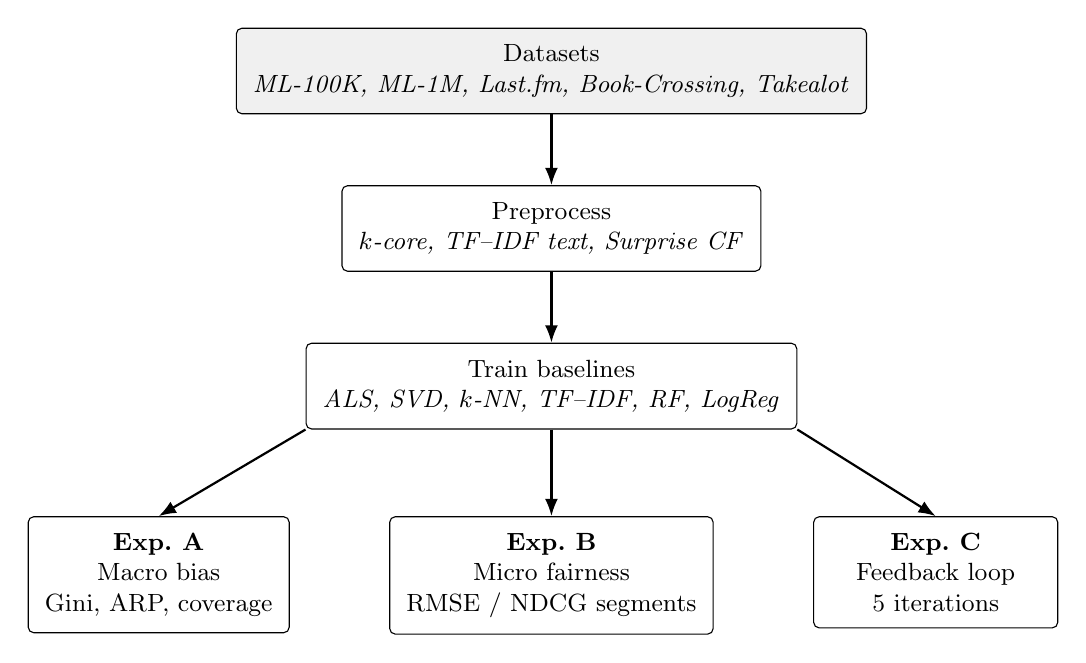
\begin{tikzpicture}[
    font=\small,
    box/.style={draw, rounded corners=2pt, align=center, inner sep=6pt, minimum width=3.1cm},
    arr/.style={-{Latex[length=2.2mm]}, thick}
  ]
    \node[box, fill=gray!12] (data) {Datasets\\\textit{ML-100K, ML-1M, Last.fm, Book-Crossing, Takealot}};
    \node[box, below=0.9cm of data] (prep) {Preprocess\\\textit{$k$-core, TF--IDF text, Surprise CF}};
    \node[box, below=0.9cm of prep] (train) {Train baselines\\\textit{ALS, SVD, $k$-NN, TF--IDF, RF, LogReg}};
    \node[box, below left=1.1cm and 0.2cm of train] (a) {\textbf{Exp.~A}\\Macro bias\\Gini, ARP, coverage};
    \node[box, below=1.1cm of train] (b) {\textbf{Exp.~B}\\Micro fairness\\RMSE / NDCG segments};
    \node[box, below right=1.1cm and 0.2cm of train] (c) {\textbf{Exp.~C}\\Feedback loop\\5 iterations};
    \draw[arr] (data) -- (prep);
    \draw[arr] (prep) -- (train);
    \draw[arr] (train.south west) -- (a.north);
    \draw[arr] (train.south) -- (b.north);
    \draw[arr] (train.south east) -- (c.north);
  \end{tikzpicture}
  \caption{Unified pipeline: shared preprocessing and model training feed three evaluation tracks (Chapters~\ref{ch:exp_a}--\ref{ch:exp_c}).}
  \label{fig:app-pipeline}
\end{figure}

\section{Stylised feedback loop with explicit simulator knobs}
Figure~\ref{fig:app-feedback-schematic} summarises the feedback simulation at the level of state variables referenced in Chapter~\ref{ch:exp_c}. Clicks use the linear blend $c_{ui}=\mathrm{clip}(0.7\, s_{ui}+0.3\, \tilde{p}_i,[0,1])$ from Section~\ref{sec:method_click}, then a Bernoulli draw on each recommended slot.

\begin{figure}[p]
  \centering
  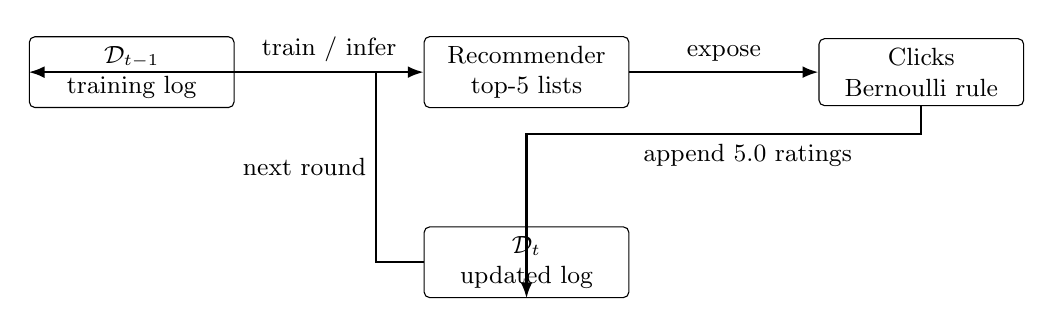
\begin{tikzpicture}[
    font=\small,
    n/.style={draw, circle, minimum size=1.05cm, inner sep=0pt},
    sq/.style={draw, rounded corners=2pt, minimum width=2.6cm, minimum height=0.85cm, align=center},
    arr/.style={-{Latex[length=2mm]}, thick}
  ]
    \node[sq] (log) {$\mathcal{D}_{t-1}$\\training log};
    \node[sq, right=2.4cm of log] (rec) {Recommender\\top-$5$ lists};
    \node[sq, right=2.4cm of rec] (clk) {Clicks\\Bernoulli rule};
    \node[sq, below=1.5cm of rec] (logp) {$\mathcal{D}_t$\\updated log};
    \draw[arr] (log) -- node[above]{train / infer} (rec);
    \draw[arr] (rec) -- node[above]{expose} (clk);
    \draw[arr] (clk.south) -- ++(0,-0.35) -| node[pos=0.22, below]{append $5.0$ ratings} (logp.south);
    \draw[arr] (logp.west) -- ++(-0.6,0) |- node[pos=0.25, left]{next round} (log.west);
  \end{tikzpicture}
  \caption{Longitudinal simulator: logs evolve from recommendations and stochastic clicks, then re-enter training.}
  \label{fig:app-feedback-schematic}
\end{figure}

\section{Cross-dataset figures (same assets as the main text)}
For convenience, the heatmaps and segment plots used in Chapters~\ref{ch:exp_a}--\ref{ch:exp_c} are repeated here without reinterpretation.

\begin{figure}[p]
  \centering
  
\includegraphics[width=\linewidth]{combined_macro_gini_heatmap.png}
  \caption[Appendix: Gini heatmap]{Gini coefficient of recommendation frequency versus item popularity (all non-Takealot benchmarks).}
\end{figure}

\begin{figure}[p]
  \centering
  
\includegraphics[width=\linewidth]{combined_macro_catalog_coverage_heatmap.png}
  \caption[Appendix: catalog coverage heatmap]{Catalog coverage of top-$N$ recommendations across datasets and models.}
\end{figure}

\begin{figure}[p]
  \centering
  
\includegraphics[width=0.92\textwidth]{combined_fairness_gap_delta_rmse.png}
  \caption[Appendix: niche RMSE gap]{Niche minus mainstream RMSE ($\Delta$RMSE) by dataset and model.}
\end{figure}

\begin{figure}[p]
  \centering
  
\includegraphics[width=0.92\textwidth]{combined_rmse_niche_vs_mainstream.png}
  \caption[Appendix: RMSE by segment]{RMSE for niche versus mainstream taste segments.}
\end{figure}

\begin{figure}[p]
  \centering
  
\includegraphics[width=0.92\textwidth]{combined_feedback_diversity_decay.png}
  \caption[Appendix: feedback diversity]{Aggregate diversity and ARP across five feedback iterations (SVD versus TF--IDF).}
\end{figure}

\chapter{Extended software specifications}
\label{appendix:software}

\section{Repository layout}
All experiments are implemented as a single Python package-style tree under \texttt{Thesis\_Research/}: \texttt{run\_all.py} orchestrates dataset ingestion, training, evaluation, plotting, and CSV exports; \texttt{src/} holds metric utilities and statistical tests; \texttt{outputs/results/} stores the tables consumed by this document. Figures are written to \texttt{outputs/figures/} (and mirrored under \texttt{Thesis-main/outputs/figures/} when syncing for \LaTeX).

\begin{figure}[htbp]
  \centering
  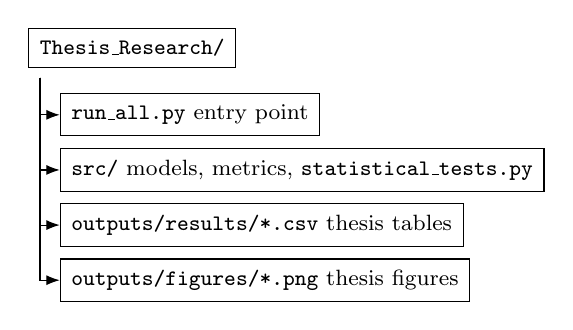
\begin{tikzpicture}[
    font=\footnotesize,
    every node/.style={draw, align=left, anchor=west, inner sep=4pt}
  ]
    \node (r) at (0,0) {\texttt{Thesis\_Research/}};
    \node (run) at (0.4,-0.85) {\texttt{run\_all.py}   entry point};
    \node (src) at (0.4,-1.55) {\texttt{src/}   models, metrics, \texttt{statistical\_tests.py}};
    \node (out) at (0.4,-2.25) {\texttt{outputs/results/*.csv}   thesis tables};
    \node (fig) at (0.4,-2.95) {\texttt{outputs/figures/*.png}   thesis figures};
    \draw[-{Latex}] (r.south west) ++(0.15,-0.12) |- (run.west);
    \draw[-{Latex}] (r.south west) ++(0.15,-0.12) |- (src.west);
    \draw[-{Latex}] (r.south west) ++(0.15,-0.12) |- (out.west);
    \draw[-{Latex}] (r.south west) ++(0.15,-0.12) |- (fig.west);
  \end{tikzpicture}
  \caption{Code and artefact layout relative to the research repository root.}
  \label{fig:app-repo-layout}
\end{figure}

\section{Language runtime and hardware assumptions}
The code targets \textbf{Python 3.10+} (tested on 64-bit Windows~10/11). Experiments are CPU-bound; GPU acceleration is not required. Wall-clock runtime scales with Book-Crossing and Takealot matrix sizes; a full multi-dataset sweep completes overnight on a modern laptop when Surprise and implicit builds are already compiled.

\section{Core dependency pins}
Table~\ref{tab:app-deps} lists the libraries that materially affect numerical results. A broader scientific stack (Jupyter, widgets, conda solver libraries) may be present in a full Anaconda install but does not change the reported metrics.

\begin{table}[htbp]
  \centering
  \small
  \begin{tabular}{@{}llp{6.8cm}@{}}
    \toprule
    \textbf{Package} & \textbf{Role in this thesis} & \textbf{Notes} \\
    \midrule
    \texttt{numpy} & Arrays, linear algebra & Pinned below 2.x for \texttt{implicit} compatibility. \\
    \texttt{pandas} & CSV aggregation & Used for all combined result tables. \\
    \texttt{scipy} & Statistics & Welch/Mann--Whitney helpers in \texttt{statistical\_tests.py}. \\
    \texttt{scikit-learn} & TF--IDF, RF, LogReg, metrics & Pipelines mirror standard sklearn idioms. \\
    \texttt{scikit-surprise} & SVD, $k$-NN, ALS & Optional import guarded when wheels are unavailable. \\
    \texttt{implicit} & ALS (implicit feedback path) & Used where the benchmark supports implicit-style training. \\
    \texttt{matplotlib}, \texttt{seaborn} & Plots & Heatmaps and line charts exported to PNG. \\
    \texttt{tqdm} & Progress bars & Long Takealot sweeps remain observable during batch runs. \\
    \bottomrule
  \end{tabular}
  \caption{Scientific stack directly exercised by \texttt{run\_all.py}.}
  \label{tab:app-deps}
\end{table}

\section{Pinned versions (\texttt{pip freeze} excerpt)}
Listing~\ref{lst:app-freeze} lists pinned versions from the development host. Reproduce with a clean virtual environment and the research repository \path{requirements.txt}, then align versions as needed.

\lstset{basicstyle=\ttfamily\footnotesize,frame=single,breaklines=true,columns=fullflexible}
\lstinputlisting[caption={Excerpted \texttt{pip} pins for core scientific dependencies.},label={lst:app-freeze}]{thesis_core_environment.txt}

\section{Regeneration checklist}
\begin{enumerate}
  \item Install dependencies from \path{requirements.txt} in the research repo; verify \texttt{surprise} imports.
  \item From the repo root, run \texttt{python run\_all.py} with the thesis defaults (top-$10$ lists for offline metrics; feedback uses top-$5$ and five iterations).
  \item Copy new PNGs into folder \path{Thesis-main/outputs/figures/} when compiling the thesis locally.
  \item Run \texttt{python scripts/export\_appendix\_tables.py} to rebuild \path{_appendix_generated_tables.tex}.
  \item Recompile \texttt{thesis.tex} (\texttt{pdflatex}, \texttt{bibtex}, \texttt{pdflatex} $\times 2$).
\end{enumerate}


\end{document}